% Options for packages loaded elsewhere
\PassOptionsToPackage{unicode}{hyperref}
\PassOptionsToPackage{hyphens}{url}
\documentclass[
  spanish,
  11pt,
]{report}
\usepackage{xcolor}
\usepackage[margin=2.5cm]{geometry}
\usepackage{amsmath,amssymb}
\setcounter{secnumdepth}{-\maxdimen} % remove section numbering
\usepackage{iftex}
\ifPDFTeX
  \usepackage[T1]{fontenc}
  \usepackage[utf8]{inputenc}
  \usepackage{textcomp} % provide euro and other symbols
\else % if luatex or xetex
  \usepackage{unicode-math} % this also loads fontspec
  \defaultfontfeatures{Scale=MatchLowercase}
  \defaultfontfeatures[\rmfamily]{Ligatures=TeX,Scale=1}
\fi
\usepackage{lmodern}
\ifPDFTeX\else
  % xetex/luatex font selection
  \setmainfont[]{Latin Modern Roman}
\fi
% Use upquote if available, for straight quotes in verbatim environments
\IfFileExists{upquote.sty}{\usepackage{upquote}}{}
\IfFileExists{microtype.sty}{% use microtype if available
  \usepackage[]{microtype}
  \UseMicrotypeSet[protrusion]{basicmath} % disable protrusion for tt fonts
}{}
\makeatletter
\@ifundefined{KOMAClassName}{% if non-KOMA class
  \IfFileExists{parskip.sty}{%
    \usepackage{parskip}
  }{% else
    \setlength{\parindent}{0pt}
    \setlength{\parskip}{6pt plus 2pt minus 1pt}}
}{% if KOMA class
  \KOMAoptions{parskip=half}}
\makeatother
\usepackage{color}
\usepackage{fancyvrb}
\newcommand{\VerbBar}{|}
\newcommand{\VERB}{\Verb[commandchars=\\\{\}]}
\DefineVerbatimEnvironment{Highlighting}{Verbatim}{commandchars=\\\{\}}
% Add ',fontsize=\small' for more characters per line
\newenvironment{Shaded}{}{}
\newcommand{\AlertTok}[1]{\textcolor[rgb]{1.00,0.00,0.00}{\textbf{#1}}}
\newcommand{\AnnotationTok}[1]{\textcolor[rgb]{0.38,0.63,0.69}{\textbf{\textit{#1}}}}
\newcommand{\AttributeTok}[1]{\textcolor[rgb]{0.49,0.56,0.16}{#1}}
\newcommand{\BaseNTok}[1]{\textcolor[rgb]{0.25,0.63,0.44}{#1}}
\newcommand{\BuiltInTok}[1]{\textcolor[rgb]{0.00,0.50,0.00}{#1}}
\newcommand{\CharTok}[1]{\textcolor[rgb]{0.25,0.44,0.63}{#1}}
\newcommand{\CommentTok}[1]{\textcolor[rgb]{0.38,0.63,0.69}{\textit{#1}}}
\newcommand{\CommentVarTok}[1]{\textcolor[rgb]{0.38,0.63,0.69}{\textbf{\textit{#1}}}}
\newcommand{\ConstantTok}[1]{\textcolor[rgb]{0.53,0.00,0.00}{#1}}
\newcommand{\ControlFlowTok}[1]{\textcolor[rgb]{0.00,0.44,0.13}{\textbf{#1}}}
\newcommand{\DataTypeTok}[1]{\textcolor[rgb]{0.56,0.13,0.00}{#1}}
\newcommand{\DecValTok}[1]{\textcolor[rgb]{0.25,0.63,0.44}{#1}}
\newcommand{\DocumentationTok}[1]{\textcolor[rgb]{0.73,0.13,0.13}{\textit{#1}}}
\newcommand{\ErrorTok}[1]{\textcolor[rgb]{1.00,0.00,0.00}{\textbf{#1}}}
\newcommand{\ExtensionTok}[1]{#1}
\newcommand{\FloatTok}[1]{\textcolor[rgb]{0.25,0.63,0.44}{#1}}
\newcommand{\FunctionTok}[1]{\textcolor[rgb]{0.02,0.16,0.49}{#1}}
\newcommand{\ImportTok}[1]{\textcolor[rgb]{0.00,0.50,0.00}{\textbf{#1}}}
\newcommand{\InformationTok}[1]{\textcolor[rgb]{0.38,0.63,0.69}{\textbf{\textit{#1}}}}
\newcommand{\KeywordTok}[1]{\textcolor[rgb]{0.00,0.44,0.13}{\textbf{#1}}}
\newcommand{\NormalTok}[1]{#1}
\newcommand{\OperatorTok}[1]{\textcolor[rgb]{0.40,0.40,0.40}{#1}}
\newcommand{\OtherTok}[1]{\textcolor[rgb]{0.00,0.44,0.13}{#1}}
\newcommand{\PreprocessorTok}[1]{\textcolor[rgb]{0.74,0.48,0.00}{#1}}
\newcommand{\RegionMarkerTok}[1]{#1}
\newcommand{\SpecialCharTok}[1]{\textcolor[rgb]{0.25,0.44,0.63}{#1}}
\newcommand{\SpecialStringTok}[1]{\textcolor[rgb]{0.73,0.40,0.53}{#1}}
\newcommand{\StringTok}[1]{\textcolor[rgb]{0.25,0.44,0.63}{#1}}
\newcommand{\VariableTok}[1]{\textcolor[rgb]{0.10,0.09,0.49}{#1}}
\newcommand{\VerbatimStringTok}[1]{\textcolor[rgb]{0.25,0.44,0.63}{#1}}
\newcommand{\WarningTok}[1]{\textcolor[rgb]{0.38,0.63,0.69}{\textbf{\textit{#1}}}}
\usepackage{longtable,booktabs,array}
\newcounter{none} % for unnumbered tables
\usepackage{calc} % for calculating minipage widths
% Correct order of tables after \paragraph or \subparagraph
\usepackage{etoolbox}
\makeatletter
\patchcmd\longtable{\par}{\if@noskipsec\mbox{}\fi\par}{}{}
\makeatother
% Allow footnotes in longtable head/foot
\IfFileExists{footnotehyper.sty}{\usepackage{footnotehyper}}{\usepackage{footnote}}
\makesavenoteenv{longtable}
\usepackage{graphicx}
\makeatletter
\newsavebox\pandoc@box
\newcommand*\pandocbounded[1]{% scales image to fit in text height/width
  \sbox\pandoc@box{#1}%
  \Gscale@div\@tempa{\textheight}{\dimexpr\ht\pandoc@box+\dp\pandoc@box\relax}%
  \Gscale@div\@tempb{\linewidth}{\wd\pandoc@box}%
  \ifdim\@tempb\p@<\@tempa\p@\let\@tempa\@tempb\fi% select the smaller of both
  \ifdim\@tempa\p@<\p@\scalebox{\@tempa}{\usebox\pandoc@box}%
  \else\usebox{\pandoc@box}%
  \fi%
}
% Set default figure placement to htbp
\def\fps@figure{htbp}
\makeatother
\ifLuaTeX
\usepackage[bidi=basic,shorthands=off]{babel}
\else
\usepackage[bidi=default,shorthands=off]{babel}
\fi
\ifPDFTeX
\else
\babelfont{rm}[]{Latin Modern Roman}
\fi
\ifLuaTeX
  \usepackage{selnolig} % disable illegal ligatures
\fi
\setlength{\emergencystretch}{3em} % prevent overfull lines
\providecommand{\tightlist}{%
  \setlength{\itemsep}{0pt}\setlength{\parskip}{0pt}}
\usepackage{bookmark}
\IfFileExists{xurl.sty}{\usepackage{xurl}}{} % add URL line breaks if available
\urlstyle{same}
\hypersetup{
  pdftitle={Documentación Ziryab --- Confluence y Manuales de Usuario},
  pdfauthor={Equipo Sonrisa --- TFG Ziryab},
  pdflang={es},
  hidelinks,
  pdfcreator={LaTeX via pandoc}}

\title{Documentación Ziryab --- Confluence y Manuales de Usuario}
\author{Equipo Sonrisa --- TFG Ziryab}
\date{Junio 2026}

\begin{document}
\maketitle

{
\setcounter{tocdepth}{2}
\tableofcontents
}
\chapter{Documentación Ziryab}\label{documentaciuxf3n-ziryab}

Exportación Confluence (espacio Ziryab) y manuales de usuario.

\chapter{Parte I --- Documentación
Confluence}\label{parte-i-documentaciuxf3n-confluence}

\section{Project Charter}\label{project-charter}

\textbf{Origen:}
https://g-team-ddm5j4dr.atlassian.net/wiki/spaces/Ziryab/pages/2261253\\
\textbf{ID página:} 2261253\\
\textbf{Última versión:} 6

\begin{center}\rule{0.5\linewidth}{0.5pt}\end{center}

\section{Nuestra idea}\label{nuestra-idea}

La aplicación \textbf{Ziryab} será el futuro para la \textbf{gestión en
centros educativos}, \textbf{sencilla}, de \textbf{fácil manejo,
amigable al usuario} y \textbf{completa}. Esta aplicación permitirá a
los \textbf{profesionales de la educación} ---ya sean
\textbf{profesores}, \textbf{orientadores}, \textbf{personal auxiliar
y/o administrativo}, así como a los \textbf{estudiantes} y sus
\textbf{padres} o \textbf{tutores}--- una gestión integral desde un
mismo entorno.

\subsection{Por el lado de los
profesores}\label{por-el-lado-de-los-profesores}

\begin{itemize}
\tightlist
\item
  \textbf{Organizar las clases}, mandar y recibir tareas.
\item
  \textbf{Calificar tareas y exámenes}.
\item
  \textbf{Controlar la asistencia} de los estudiantes.
\item
  \textbf{Comunicarse con padres o tutores}.
\item
  \textbf{Comunicarse internamente} entre profesores, ya sea de
  \textbf{forma libre}, por \textbf{departamentos} o con la
  \textbf{administración} del \textbf{centro}.
\end{itemize}

A los profesores que también ocupen \textbf{cargos administrativos} como
\textbf{secretaría}, \textbf{jefatura de estudios} o \textbf{dirección},
se les dará la opción de \textbf{gestionar todo su trabajo desde la
misma aplicación}, al estar identificados no solo como docentes sino
también por su \textbf{puesto específico}.

En el caso de personal con \textbf{únicamente tareas administrativas},
tendrán acceso directo a sus funciones desde la aplicación.

Además, Ziryab tendrá en cuenta al \textbf{personal de educación
especial}, tanto de \textbf{centros especializados} como de
\textbf{alumnos integrados en centros generales}, ofreciendo
\textbf{facilidades para la comunicación con padres y alumnos} y
\textbf{adaptándose} a \textbf{diferentes tipos de discapacidad}.

\subsection{Por el lado de los
alumnos}\label{por-el-lado-de-los-alumnos}

\begin{itemize}
\tightlist
\item
  \textbf{Acceder} a \textbf{todas} las \textbf{asignaturas o módulos}
  cursados.
\item
  Consultar \textbf{temarios}, \textbf{tareas} y
  \textbf{calificaciones}.
\item
  \textbf{Conocer} en todo momento el \textbf{estado del curso}.
\item
  \textbf{Gestionar} la \textbf{firma} y \textbf{recepción de
  documentos}.
\item
  \textbf{Controlar} y \textbf{justificar asistencias} y
  \textbf{ausencias}.
\end{itemize}

\subsection{Parte administrativa}\label{parte-administrativa}

\begin{itemize}
\tightlist
\item
  \textbf{Matriculación}.
\item
  \textbf{Gestión} de \textbf{becas} y \textbf{solicitudes}.
\item
  \textbf{Comunicación} con \textbf{profesores} o \textbf{departamento
  de orientación}.
\item
  \textbf{Entrega} y \textbf{recepción} de \textbf{documentación}.
\end{itemize}

Todo esto estará acompañado por una \textbf{interfaz adaptada a
cualquier situación de dificultad por parte de los usuarios}.

En casos especiales, Ziryab permitirá la \textbf{interacción directa
entre alumnado}, \textbf{profesorado} y \textbf{tutores} siempre que sea
necesario.

\section{Project Charter (imagen)}\label{project-charter-imagen}

\begin{quote}
Imagen del charter en Confluence --- exportar manualmente desde la
página online si hace falta en el PDF.
\end{quote}

\section{Diagrama base de datos}\label{diagrama-base-de-datos}

\begin{quote}
Diagrama ER en Confluence --- ver también
\texttt{node/prisma/esquema-relacional.md} en el repositorio backend.
\end{quote}

\section{Prototipos Figma}\label{prototipos-figma}

\begin{itemize}
\tightlist
\item
  \href{https://g-team-ddm5j4dr.atlassian.net/wiki/spaces/Ziryab/pages/2261253\#Prototipo-PC}{Prototipo
  a PC}
\item
  \href{https://www.figma.com/proto/j1rFThKhIcsvGUbp0JYK7U/Ziryab?page-id=0\%3A1&node-id=35-93&p=f&viewport=-3034\%2C71\%2C0.56&t=mgKuJhBCeqkAkSzV-1&scaling=scale-down&content-scaling=fixed&starting-point-node-id=35\%3A93}{Prototipo
  a móvil}
\end{itemize}

\section{Objetivos SMART}\label{objetivos-smart}

\subsection{Comunicación Alumno
Profesor}\label{comunicaciuxf3n-alumno-profesor}

Implementar un sistema de retroalimentación semanal entre alumno y
profesor, mediante un formulario digital, para mejorar la claridad en la
entrega de instrucciones y resolución de dudas, alcanzando al menos un
80\% de participación de los estudiantes durante los próximos tres
meses.

\begin{itemize}
\tightlist
\item
  \textbf{Qué/Para quién (S)}: Implementar un sistema de
  retroalimentación semanal mediante formulario digital entre alumno y
  profesor para todos los estudiantes.
\item
  \textbf{Medida de éxito (M)}: alcanzar ≥ 80\% de participación
  estudiantil cada semana durante tres meses; feedback recogido en
  \textgreater{} 10 de 13 semanas posibles.
\item
  \textbf{Viabilidad (A)}: usando Google Forms y notificaciones por
  email; esfuerzo estimado 6 h diseño/implantación + 1 h/sem
  mantenimiento.
\item
  \textbf{Relevancia (R)}: mejora la claridad de instrucciones y dudas
  resueltas a tiempo, aumentando satisfacción y rendimiento académico.
\item
  \textbf{Plazo (T)}: durante los próximos 3 meses (octubre--diciembre);
  primera recogida antes de finalizar la semana 1.
\item
  \textbf{Entregables}: formulario digital, resultados semanales
  (dashboards), resumen mensual para profesorado, evidencia de
  envíos/participación.
\item
  \textbf{Riesgos y mitigación}: baja participación → recordatorios
  automáticos y feedback anónimo; problemas técnicos → soporte rápido
  con plantillas alternativas.
\end{itemize}

\subsection{Gestión del curso escolar por parte del
profesor}\label{gestiuxf3n-del-curso-escolar-por-parte-del-profesor}

Organizar y publicar en la plataforma educativa el plan de trabajo
trimestral con fechas de entrega y criterios de evaluación, asegurando
que esté disponible y actualizado el primer día de cada trimestre
durante todo el curso.

\begin{itemize}
\tightlist
\item
  \textbf{Qué/Para quién (S)}: Organizar y publicar en la plataforma
  educativa (para todos los alumnos y padres) el plan de trabajo
  trimestral, incluyendo fechas de entrega y criterios de evaluación.
\item
  \textbf{Medida de éxito (M)}: el plan debe estar online y accesible el
  primer día de cada trimestre, actualizado al 100\% de los trimestres;
  notificaciones emitidas a todos los destinatarios.
\item
  \textbf{Viabilidad (A)}: usando la función ``Materiales'' de la
  plataforma educativa, esfuerzo estimado 4 h por trimestre para
  preparación y subida.
\item
  \textbf{Relevancia (R)}: asegura la transparencia y previsión para
  estudiantes y familias.
\item
  \textbf{Plazo (T)}: publicación antes de las 8:00 h del primer día
  lectivo de cada trimestre.
\item
  \textbf{Entregables}: documento o sección del plan disponible en la
  plataforma, registro de acceso/descarga por al menos el 90\% de las
  familias/estudiantes.
\end{itemize}

\subsection{Gestión administrativa para el
alumnado}\label{gestiuxf3n-administrativa-para-el-alumnado}

Digitalizar y centralizar el acceso a documentos administrativos
(certificados, solicitudes y horarios) en un portal único para los
estudiantes, alcanzando un 90\% de uso regular por parte del alumnado en
un plazo de seis meses.

\begin{itemize}
\tightlist
\item
  \textbf{Qué/Para quién (S)}: Portal único para todos los estudiantes.
\item
  \textbf{Medida de éxito (M)}: ≥ 90\% de uso regular en seis meses.
\item
  \textbf{Viabilidad (A)}: portal web con credenciales institucionales;
  desarrollo estimado 24 h.
\item
  \textbf{Relevancia (R)}: agiliza trámites y reduce papeleo.
\item
  \textbf{Plazo (T)}: 6 meses tras el lanzamiento.
\item
  \textbf{Entregables}: portal en funcionamiento, registros de acceso,
  manual de usuario, encuesta de satisfacción.
\end{itemize}

\section{Inicio de servidores Angular y
Node}\label{inicio-de-servidores-angular-y-node}

\textbf{Origen:}
https://g-team-ddm5j4dr.atlassian.net/wiki/spaces/Ziryab/pages/9404417\\
\textbf{ID página:} 9404417

\begin{center}\rule{0.5\linewidth}{0.5pt}\end{center}

\section{Objetivo}\label{objetivo}

Documentar los pasos necesarios para configurar el entorno de desarrollo
e iniciar los servidores de backend (Node.js 19) y frontend (Angular
19), incluyendo configuración de variables de entorno, instalación de
dependencias y herramientas relacionadas con Firebase.

\section{Prerrequisitos}\label{prerrequisitos}

\begin{itemize}
\tightlist
\item
  Node.js versión 19 instalada.
\item
  Angular CLI compatible con Angular 19 (recomendada instalación
  global).
\item
  Acceso al repositorio de los proyectos (Node y Angular).
\item
  Credenciales necesarias para Firebase y otros servicios.
\end{itemize}

\begin{center}\rule{0.5\linewidth}{0.5pt}\end{center}

\section{Configuración de variables de entorno
(.env)}\label{configuraciuxf3n-de-variables-de-entorno-.env}

\subsection{Backend (Node.js 19)}\label{backend-node.js-19}

\begin{enumerate}
\def\labelenumi{\arabic{enumi}.}
\tightlist
\item
  Crear un archivo \texttt{.env} en la raíz del proyecto backend si no
  existe.
\item
  Definir variables como:

  \begin{itemize}
  \tightlist
  \item
    \texttt{PORT}
  \item
    \texttt{NODE\_ENV}
  \item
    \texttt{DB\_URL}
  \item
    Variables relacionadas con Firebase si aplica.
  \end{itemize}
\item
  Verificar que se use \texttt{dotenv} para cargar las variables al
  arrancar la app.
\end{enumerate}

\subsection{Frontend (Angular 19)}\label{frontend-angular-19}

\begin{enumerate}
\def\labelenumi{\arabic{enumi}.}
\tightlist
\item
  Configurar los archivos de entorno (\texttt{environment.ts},
  \texttt{environment.prod.ts}) o mecanismo \texttt{.env} usado por el
  proyecto, con:

  \begin{itemize}
  \tightlist
  \item
    URL de la API backend.
  \item
    Configuración Firebase (apiKey, authDomain, etc.).
  \end{itemize}
\item
  Evitar incluir datos sensibles directamente en el repositorio.
\end{enumerate}

\begin{center}\rule{0.5\linewidth}{0.5pt}\end{center}

\section{Instalación de
dependencias}\label{instalaciuxf3n-de-dependencias}

\subsection{Instalación global}\label{instalaciuxf3n-global}

\begin{itemize}
\tightlist
\item
  Angular CLI compatible con Angular 19:

  \begin{itemize}
  \tightlist
  \item
    \texttt{npm\ install\ -g\ @angular/cli@19}
  \end{itemize}
\item
  Firebase CLI para herramientas y despliegues:

  \begin{itemize}
  \tightlist
  \item
    \texttt{npm\ install\ -g\ firebase-tools}
  \end{itemize}
\end{itemize}

\subsection{Backend (Node 19)}\label{backend-node-19}

\begin{enumerate}
\def\labelenumi{\arabic{enumi}.}
\tightlist
\item
  En la carpeta backend, ejecutar \texttt{npm\ install} para
  dependencias del proyecto.
\item
  Instalar Firebase SDK si se usa:

  \begin{itemize}
  \tightlist
  \item
    \texttt{npm\ install\ firebase}
  \end{itemize}
\end{enumerate}

\subsection{Frontend (Angular 19)}\label{frontend-angular-19-1}

\begin{enumerate}
\def\labelenumi{\arabic{enumi}.}
\tightlist
\item
  En la carpeta frontend, ejecutar \texttt{npm\ install}.
\item
  Instalar Firebase SDK si se usa:

  \begin{itemize}
  \tightlist
  \item
    \texttt{npm\ install\ firebase}
  \end{itemize}
\end{enumerate}

\begin{center}\rule{0.5\linewidth}{0.5pt}\end{center}

\section{Inicio de los servidores}\label{inicio-de-los-servidores}

\subsection{Backend Node.js 19}\label{backend-node.js-19-1}

\begin{enumerate}
\def\labelenumi{\arabic{enumi}.}
\tightlist
\item
  Confirmar configuración correcta del \texttt{.env}.
\item
  Ejecutar:

  \begin{itemize}
  \tightlist
  \item
    \texttt{npm\ run\ dev} (modo desarrollo) o
  \item
    \texttt{npm\ start} (producción local).
  \end{itemize}
\item
  Verificar funcionamiento en
  \texttt{http://localhost:\textless{}PORT\textgreater{}}.
\end{enumerate}

\subsection{Frontend Angular 19}\label{frontend-angular-19-2}

\begin{enumerate}
\def\labelenumi{\arabic{enumi}.}
\tightlist
\item
  Confirmar correcto apuntado a backend vía variables de entorno.
\item
  Ejecutar:

  \begin{itemize}
  \tightlist
  \item
    \texttt{ng\ serve} o
  \item
    \texttt{npm\ run\ start}.
  \end{itemize}
\item
  Acceder a \texttt{http://localhost:4200} para probar la app Angular.
\end{enumerate}

\section{Documentación técnica Frontend
(Angular)}\label{documentaciuxf3n-tuxe9cnica-frontend-angular}

\textbf{Origen:}
https://g-team-ddm5j4dr.atlassian.net/wiki/spaces/Ziryab/pages/35028993\\
\textbf{ID página:} 35028993

\begin{center}\rule{0.5\linewidth}{0.5pt}\end{center}

Bienvenido/a a la documentación oficial del frontend de la aplicación.
Este espacio sirve como punto de entrada para desarrolladores,
arquitectos y cualquier miembro del equipo que necesite comprender la
estructura, los servicios y la arquitectura visual del proyecto.

\section{Objetivo de la
Documentación}\label{objetivo-de-la-documentaciuxf3n}

El repositorio frontend ha sido rigurosamente documentado utilizando
\textbf{Compodoc}. Nuestro objetivo es mantener un estándar de calidad
estricto para que el mantenimiento, la escalabilidad y la integración de
nuevos desarrolladores («onboarding») sea lo más ágil posible.

\begin{quote}
\textbf{Hito alcanzado:} Actualmente el código cuenta con un
\textbf{100\% de cobertura de documentación}. Todos los módulos,
componentes, servicios, guards, interfaces y directivas tienen detallado
su propósito, inicialización y retorno.
\end{quote}

\section{Acceso a la Documentación (GitHub
Pages)}\label{acceso-a-la-documentaciuxf3n-github-pages}

Toda la documentación interactiva, diagramas de módulos, árbol de
dependencias y el buscador de componentes se genera de manera
automatizada y está alojada en GitHub Pages.

\textbf{URL actual del proyecto Ziryab:}
\url{https://antoniosalces.github.io/ziryab-compodoc/index.html}

\emph{(La página Confluence enlazaba anteriormente a
\texttt{antoniosalces.github.io/documentation/}.)}

\subsection{Comandos locales}\label{comandos-locales}

\begin{Shaded}
\begin{Highlighting}[]
\BuiltInTok{cd}\NormalTok{ angular}
\ExtensionTok{npm}\NormalTok{ run docs:build    }\CommentTok{\# genera estáticos en docs/}
\ExtensionTok{npm}\NormalTok{ run docs:serve    }\CommentTok{\# servidor local para revisión}
\end{Highlighting}
\end{Shaded}

\section{Resumen gestión de
proyecto}\label{resumen-gestiuxf3n-de-proyecto}

\textbf{Origen:}
https://g-team-ddm5j4dr.atlassian.net/wiki/spaces/Ziryab/pages/13500417\\
\textbf{ID página:} 13500417

\begin{center}\rule{0.5\linewidth}{0.5pt}\end{center}

Enlace al tablero Jira del equipo:

https://g-team-ddm5j4dr.atlassian.net/jira/software/projects/EQ/summary

\begin{quote}
\textbf{Proyecto Jira:} \texttt{EQ} en el sitio
\texttt{g-team-ddm5j4dr.atlassian.net} (distinto del proyecto
\texttt{CURSO} en \texttt{franciscocobsan.atlassian.net} usado en
desarrollo con Cursor).
\end{quote}

\newpage

\chapter{Parte II --- Manual de usuario:
Alumno}\label{parte-ii-manual-de-usuario-alumno}

\textbf{Versión:} 1.0 · \textbf{Aplicación:} Ziryab --- Plataforma
Educativa\\
\textbf{Rol:} Estudiante (STUDENT)\\
\textbf{Última actualización:} junio 2026 · \textbf{Capturas:} incluidas

\begin{center}\rule{0.5\linewidth}{0.5pt}\end{center}

\section{1. Introducción}\label{introducciuxf3n}

\textbf{Ziryab} es la plataforma web del centro donde puedes consultar
tus asignaturas, entregar tareas, ver tu horario, revisar faltas de
asistencia, consultar calificaciones y leer avisos del centro.

\begin{center}\rule{0.5\linewidth}{0.5pt}\end{center}

\section{2. Requisitos previos}\label{requisitos-previos}

{\def\LTcaptype{none} % do not increment counter
\begin{longtable}[]{@{}
  >{\raggedright\arraybackslash}p{(\linewidth - 2\tabcolsep) * \real{0.5500}}
  >{\raggedright\arraybackslash}p{(\linewidth - 2\tabcolsep) * \real{0.4500}}@{}}
\toprule\noalign{}
\begin{minipage}[b]{\linewidth}\raggedright
Requisito
\end{minipage} & \begin{minipage}[b]{\linewidth}\raggedright
Detalle
\end{minipage} \\
\midrule\noalign{}
\endhead
\bottomrule\noalign{}
\endlastfoot
Navegador & Chrome, Firefox, Edge o Safari actualizado \\
Credenciales & Email y contraseña facilitados por el centro \\
Conexión & Internet estable \\
Idioma & La app admite \textbf{español}, \textbf{inglés} y
\textbf{alemán} (selector en la cabecera) \\
\end{longtable}
}

\begin{center}\rule{0.5\linewidth}{0.5pt}\end{center}

\section{3. Inicio de sesión}\label{inicio-de-sesiuxf3n}

\subsection{3.1 Acceder a la
aplicación}\label{acceder-a-la-aplicaciuxf3n}

\begin{enumerate}
\def\labelenumi{\arabic{enumi}.}
\tightlist
\item
  Abre la URL de Ziryab en el navegador (la proporciona tu centro).
\item
  Serás redirigido a la pantalla de \textbf{Inicio de sesión} si no
  tienes sesión activa.
\end{enumerate}

\begin{figure}
\centering
\pandocbounded{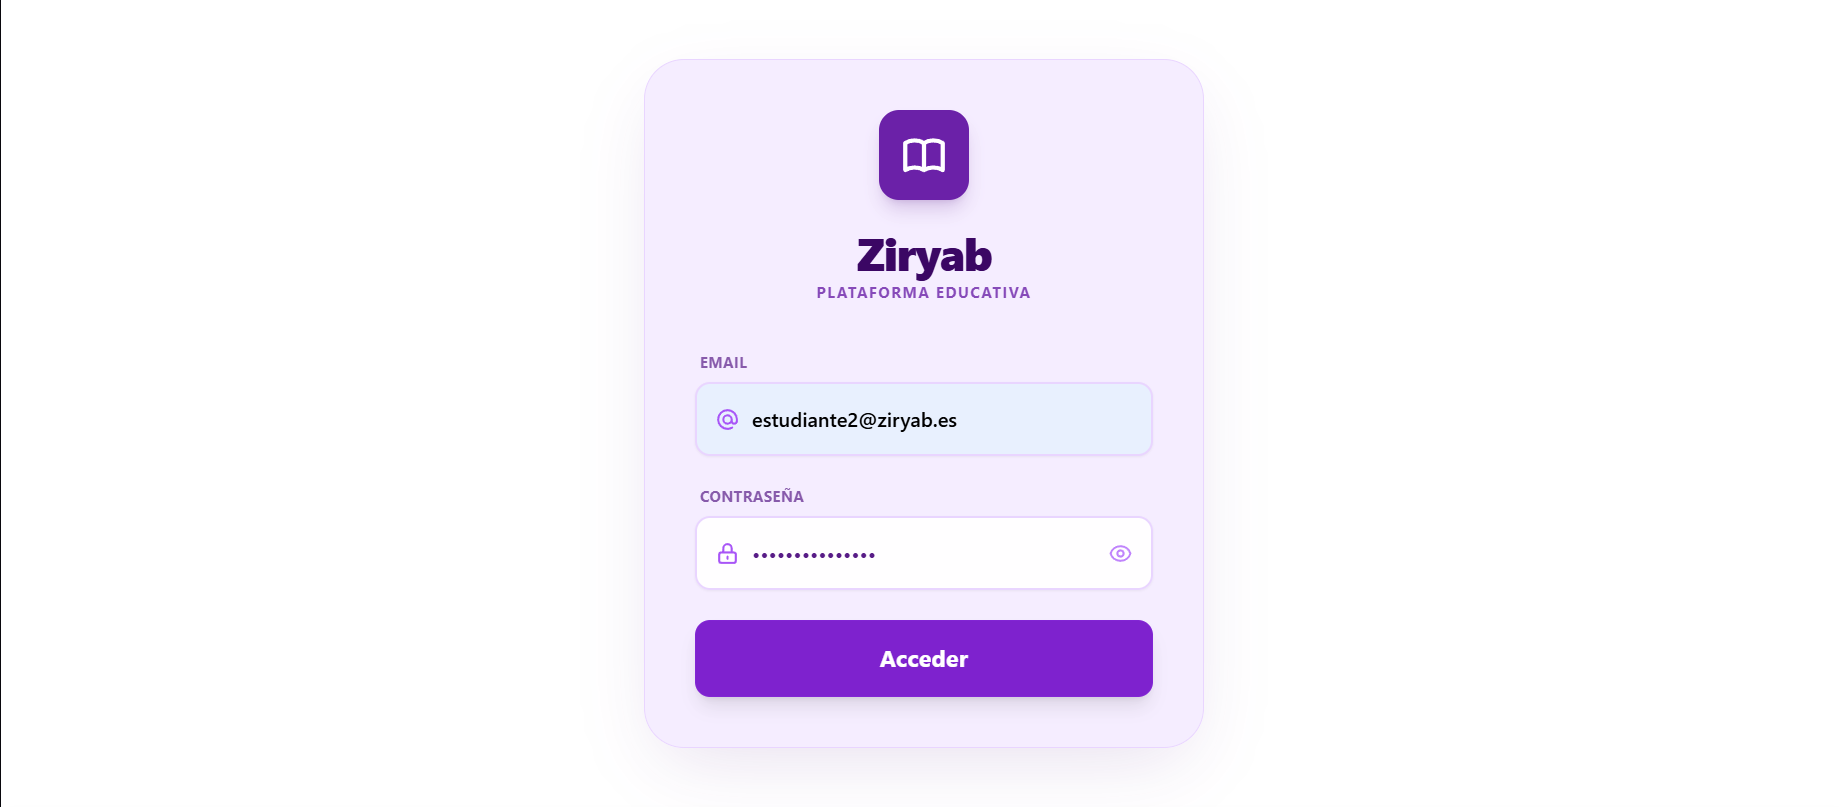
\includegraphics[keepaspectratio,alt={CAPTURA 1 --- Pantalla de login}]{../../assets/screenshots/manual-alumno/captura01-login.png}}
\caption{CAPTURA 1 --- Pantalla de login}
\end{figure}

\subsection{3.2 Introducir credenciales}\label{introducir-credenciales}

\begin{enumerate}
\def\labelenumi{\arabic{enumi}.}
\tightlist
\item
  Escribe tu \textbf{email} en el primer campo (icono de sobre).
\item
  Escribe tu \textbf{contraseña} en el segundo campo.
\item
  Opcional: pulsa el icono del ojo para \textbf{mostrar u ocultar} la
  contraseña.
\item
  Pulsa el botón principal para \textbf{acceder}.
\end{enumerate}

\subsection{3.3 Errores habituales en el
login}\label{errores-habituales-en-el-login}

\begin{itemize}
\tightlist
\item
  Si las credenciales son incorrectas, aparece un \textbf{mensaje de
  error en rojo} bajo el formulario.
\item
  Si el campo email no es válido, el formulario no enviará la petición.
\item
  Tras un login correcto, entrarás al \textbf{panel principal (Mi
  Espacio)}.
\end{itemize}

\begin{figure}
\centering
\pandocbounded{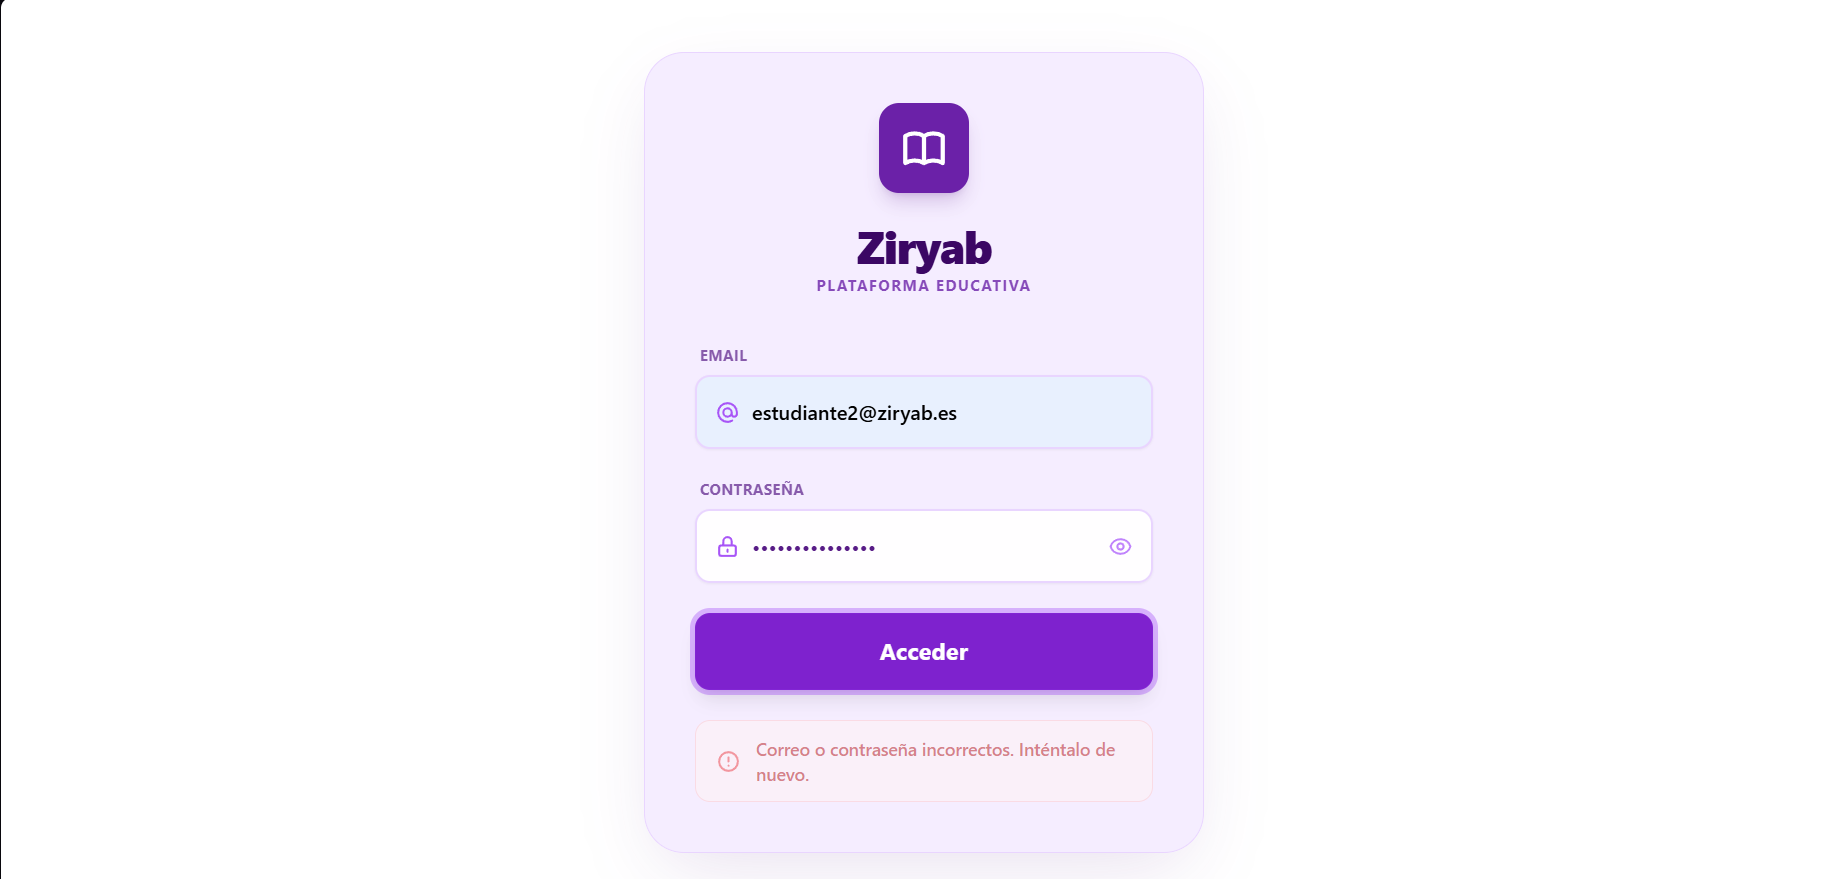
\includegraphics[keepaspectratio,alt={CAPTURA 2 --- Error de login}]{../../assets/screenshots/manual-alumno/captura02-error_login.png}}
\caption{CAPTURA 2 --- Error de login}
\end{figure}

\begin{center}\rule{0.5\linewidth}{0.5pt}\end{center}

\section{4. Interfaz general
(cabecera)}\label{interfaz-general-cabecera}

En todas las pantallas privadas verás una \textbf{cabecera morada} fija
con:

{\def\LTcaptype{none} % do not increment counter
\begin{longtable}[]{@{}
  >{\raggedright\arraybackslash}p{(\linewidth - 4\tabcolsep) * \real{0.3333}}
  >{\raggedright\arraybackslash}p{(\linewidth - 4\tabcolsep) * \real{0.3667}}
  >{\raggedright\arraybackslash}p{(\linewidth - 4\tabcolsep) * \real{0.3000}}@{}}
\toprule\noalign{}
\begin{minipage}[b]{\linewidth}\raggedright
Elemento
\end{minipage} & \begin{minipage}[b]{\linewidth}\raggedright
Ubicación
\end{minipage} & \begin{minipage}[b]{\linewidth}\raggedright
Función
\end{minipage} \\
\midrule\noalign{}
\endhead
\bottomrule\noalign{}
\endlastfoot
Selector de idioma & Izquierda & Cambia entre ES / EN / DE \\
Logotipo \textbf{Ziryab} & Centro & Al pulsar, vuelves al
\textbf{Dashboard} \\
Campana de notificaciones & Derecha & Abre el panel de notificaciones \\
Bloque de perfil (nombre + rol) & Derecha & Abre el menú de perfil \\
\end{longtable}
}

\begin{figure}
\centering
\pandocbounded{
\includegraphics[keepaspectratio,alt={CAPTURA 3 --- Cabecera de alumno}]{../../assets/screenshots/manual-alumno/captura03-cabecera.png}}
\caption{CAPTURA 3 --- Cabecera de alumno}
\end{figure}

\subsection{4.1 Notificaciones}\label{notificaciones}

\begin{enumerate}
\def\labelenumi{\arabic{enumi}.}
\tightlist
\item
  Pulsa la \textbf{campana}; se abre un panel lateral o desplegable.
\item
  Verás la lista de avisos (tareas nuevas, calificaciones, etc.).
\item
  Puedes \textbf{marcar todas como leídas} si la opción está disponible.
\item
  Al llegar una notificación en tiempo real, puede aparecer un
  \textbf{toast} (aviso flotante) en la parte inferior de la pantalla
  durante unos segundos.
\end{enumerate}

\begin{figure}
\centering
\pandocbounded{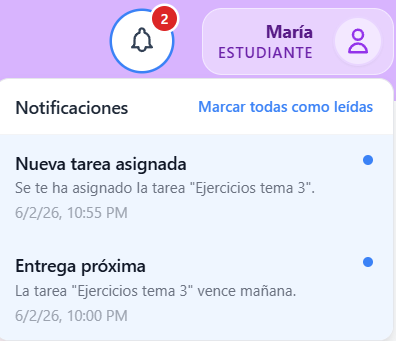
\includegraphics[keepaspectratio,alt={CAPTURA 4 --- Panel de notificaciones abierto}]{../../assets/screenshots/manual-alumno/captura04-notificaciones.png}}
\caption{CAPTURA 4 --- Panel de notificaciones abierto}
\end{figure}

\subsection{4.2 Menú de perfil y cierre de
sesión}\label{menuxfa-de-perfil-y-cierre-de-sesiuxf3n}

\begin{enumerate}
\def\labelenumi{\arabic{enumi}.}
\tightlist
\item
  Pulsa tu \textbf{nombre y avatar} en la cabecera.
\item
  Se abre un modal con tu nombre, rol y el botón \textbf{Cerrar sesión}.
\item
  Confirma el cierre; volverás a la pantalla de login.
\end{enumerate}

\begin{figure}
\centering
\pandocbounded{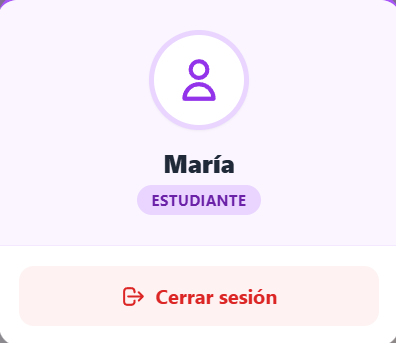
\includegraphics[keepaspectratio,alt={CAPTURA 5 --- Modal de perfil con botón Cerrar sesión}]{../../assets/screenshots/manual-alumno/captura05-modal_perfil.png}}
\caption{CAPTURA 5 --- Modal de perfil con botón Cerrar sesión}
\end{figure}

\subsection{4.3 Botón «Volver»}\label{botuxf3n-volver}

En la mayoría de pantallas secundarias aparece el componente
\textbf{Volver} (flecha atrás), que te lleva a la pantalla anterior en
el historial de navegación.

\begin{center}\rule{0.5\linewidth}{0.5pt}\end{center}

\section{5. Panel principal --- «Mi Espacio»
(Dashboard)}\label{panel-principal-mi-espacio-dashboard}

Tras iniciar sesión accedes a \textbf{Mi Espacio}, con el mensaje
\emph{«¿Qué te gustaría hacer hoy?»} y \textbf{dos tarjetas grandes}:

{\def\LTcaptype{none} % do not increment counter
\begin{longtable}[]{@{}
  >{\raggedright\arraybackslash}p{(\linewidth - 4\tabcolsep) * \real{0.2903}}
  >{\raggedright\arraybackslash}p{(\linewidth - 4\tabcolsep) * \real{0.4194}}
  >{\raggedright\arraybackslash}p{(\linewidth - 4\tabcolsep) * \real{0.2903}}@{}}
\toprule\noalign{}
\begin{minipage}[b]{\linewidth}\raggedright
Tarjeta
\end{minipage} & \begin{minipage}[b]{\linewidth}\raggedright
Descripción
\end{minipage} & \begin{minipage}[b]{\linewidth}\raggedright
Destino
\end{minipage} \\
\midrule\noalign{}
\endhead
\bottomrule\noalign{}
\endlastfoot
\textbf{Clases} & Accede a tus asignaturas matriculadas &
\texttt{/clases} \\
\textbf{Gestión} & Expediente, horario, calendario, avisos y notas &
\texttt{/gestion} \\
\end{longtable}
}

\begin{enumerate}
\def\labelenumi{\arabic{enumi}.}
\tightlist
\item
  Haz clic en la tarjeta deseada (también al pasar el ratón verás la
  etiqueta \textbf{Acceder}).
\end{enumerate}

\begin{figure}
\centering
\pandocbounded{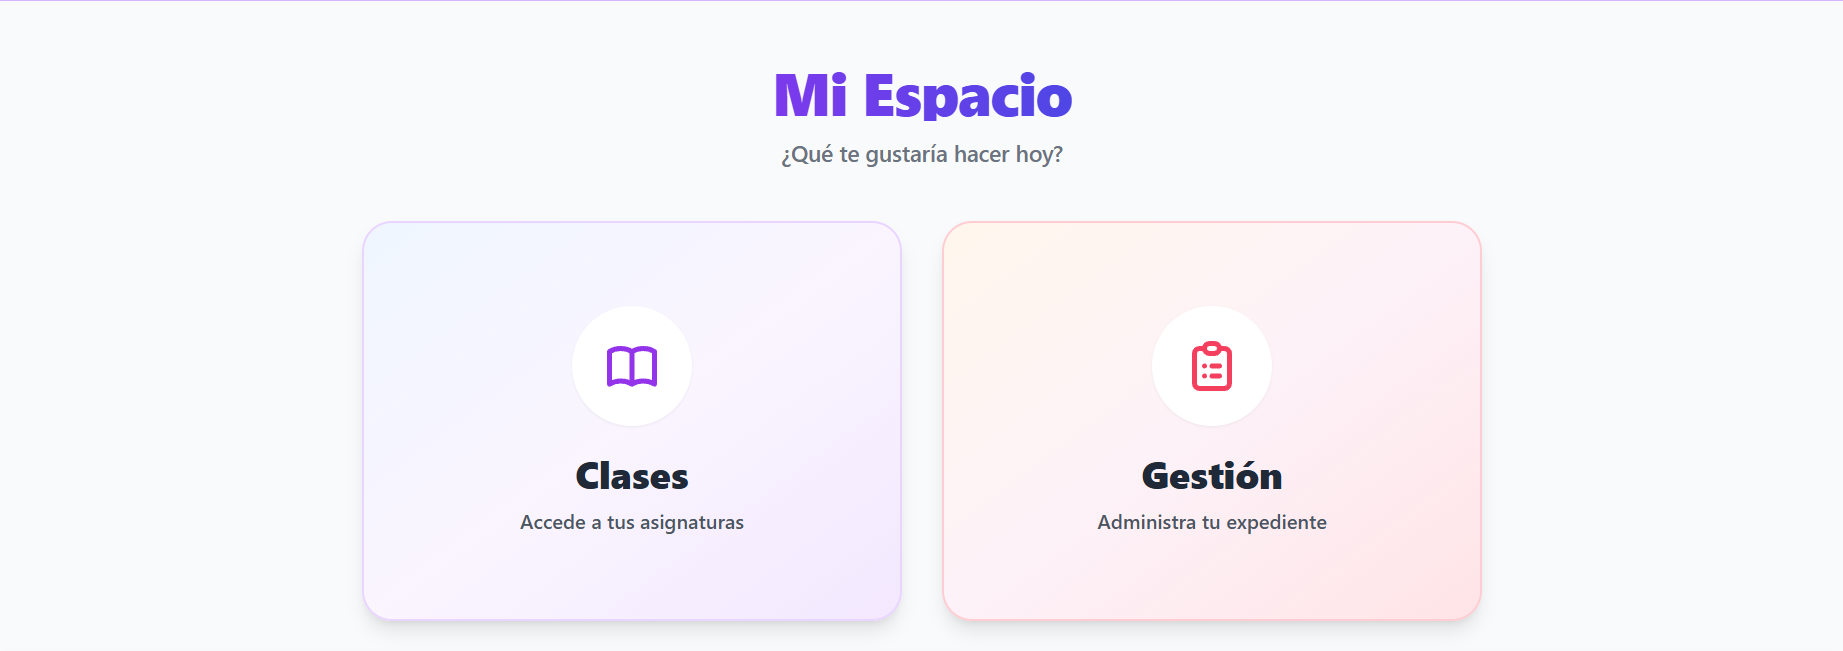
\includegraphics[keepaspectratio,alt={CAPTURA 6 --- Dashboard «Mi Espacio»}]{../../assets/screenshots/manual-alumno/captura06-dashboard.png}}
\caption{CAPTURA 6 --- Dashboard «Mi Espacio»}
\end{figure}

\begin{center}\rule{0.5\linewidth}{0.5pt}\end{center}

\section{6. Mis asignaturas (Clases)}\label{mis-asignaturas-clases}

\subsection{6.1 Listado de asignaturas}\label{listado-de-asignaturas}

Ruta: \textbf{Dashboard → Clases} (\texttt{/clases}).

\begin{itemize}
\tightlist
\item
  Verás una \textbf{rejilla de tarjetas}, una por cada asignatura en la
  que estás matriculado.
\item
  Cada tarjeta muestra, entre otros datos: \textbf{nombre de la
  asignatura}, \textbf{ciclo/curso}, \textbf{grupo} y \textbf{profesor}
  (cuando esté disponible).
\item
  Mientras carga, aparece el mensaje \emph{«Cargando tus clases\ldots»}.
\item
  Si no tienes matrículas, verás \emph{«No estás matriculado en ninguna
  asignatura»}.
\end{itemize}

\begin{figure}
\centering
\pandocbounded{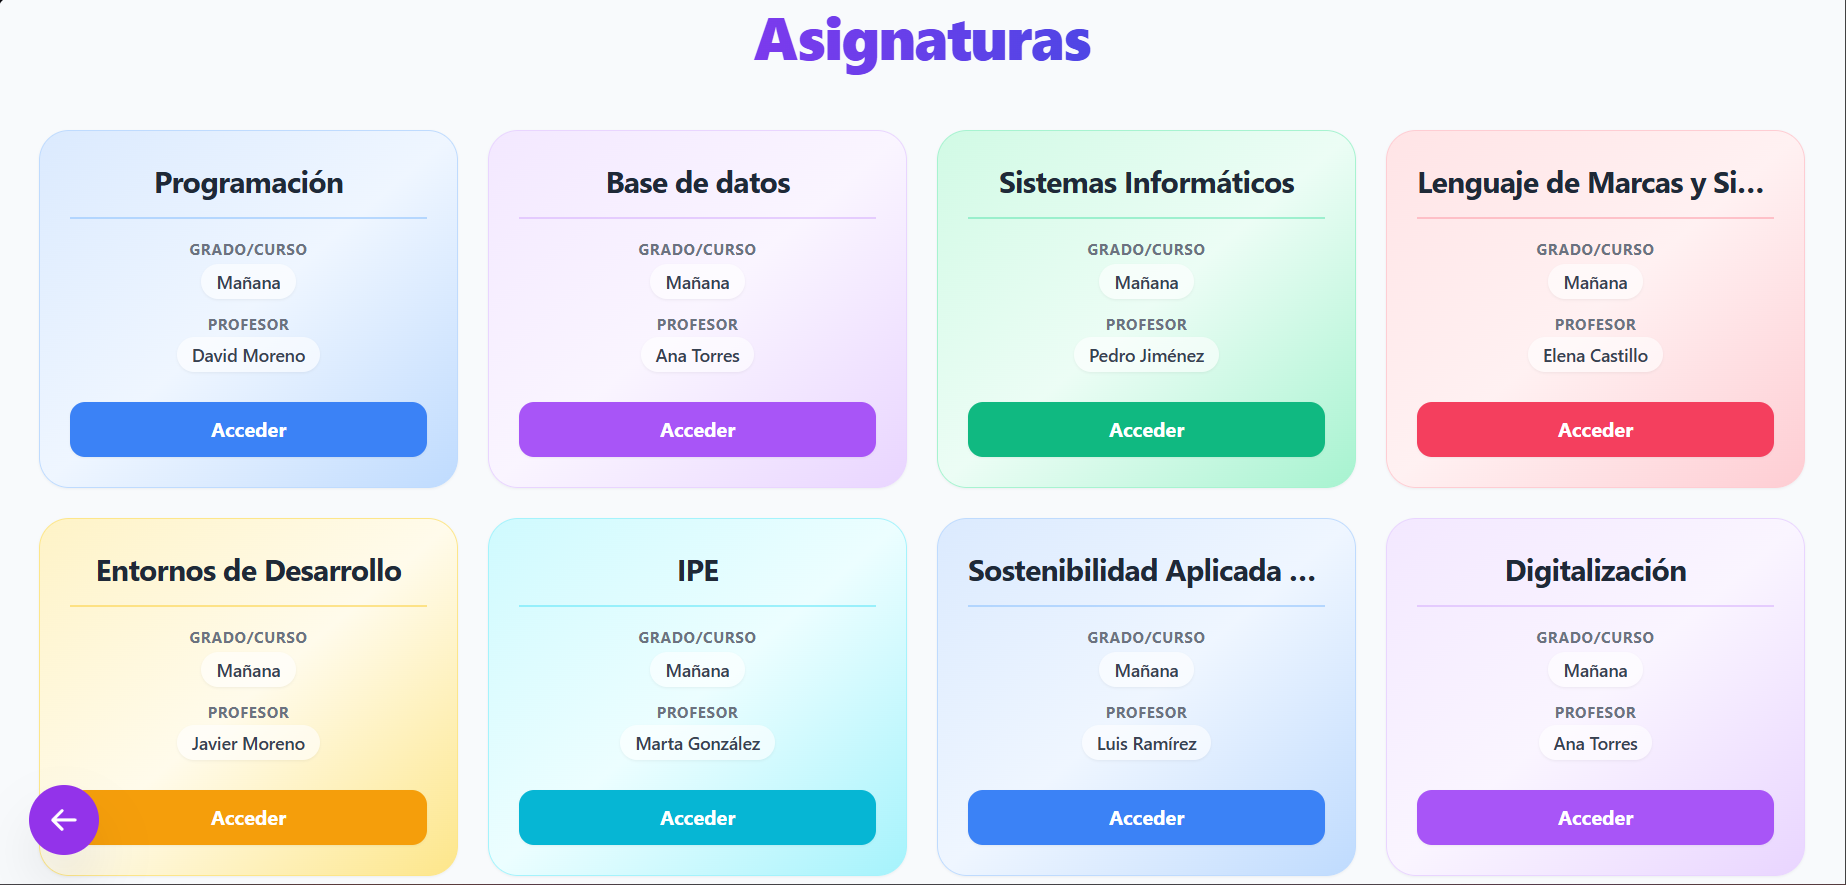
\includegraphics[keepaspectratio,alt={CAPTURA 7 --- Listado de asignaturas del alumno}]{../../assets/screenshots/manual-alumno/captura07-asignaturas.png}}
\caption{CAPTURA 7 --- Listado de asignaturas del alumno}
\end{figure}

\subsection{6.2 Entrar al temario de una
asignatura}\label{entrar-al-temario-de-una-asignatura}

\begin{enumerate}
\def\labelenumi{\arabic{enumi}.}
\tightlist
\item
  En la tarjeta de la asignatura, pulsa la acción principal (abrir /
  acceder al temario).
\item
  Irás a \textbf{Temario} (\texttt{/temario/:claseId}) con el material y
  las tareas de esa asignatura.
\end{enumerate}

\begin{center}\rule{0.5\linewidth}{0.5pt}\end{center}

\section{7. Temario y listado de
tareas}\label{temario-y-listado-de-tareas}

\subsection{7.1 Estructura del temario}\label{estructura-del-temario}

El temario organiza el contenido en \textbf{bloques desplegables} por
tipo:

\begin{itemize}
\tightlist
\item
  Material teórico y documentos\\
\item
  Exámenes y pruebas\\
\item
  Proyectos evaluables\\
\item
  Ejercicios prácticos\\
\item
  Deberes generales
\end{itemize}

\begin{enumerate}
\def\labelenumi{\arabic{enumi}.}
\tightlist
\item
  Pulsa la cabecera de un bloque para \textbf{expandirlo o contraerlo}.
\item
  Dentro verás las \textbf{tareas} con título, fecha límite y
  \textbf{estado}.
\end{enumerate}

\begin{figure}
\centering
\pandocbounded{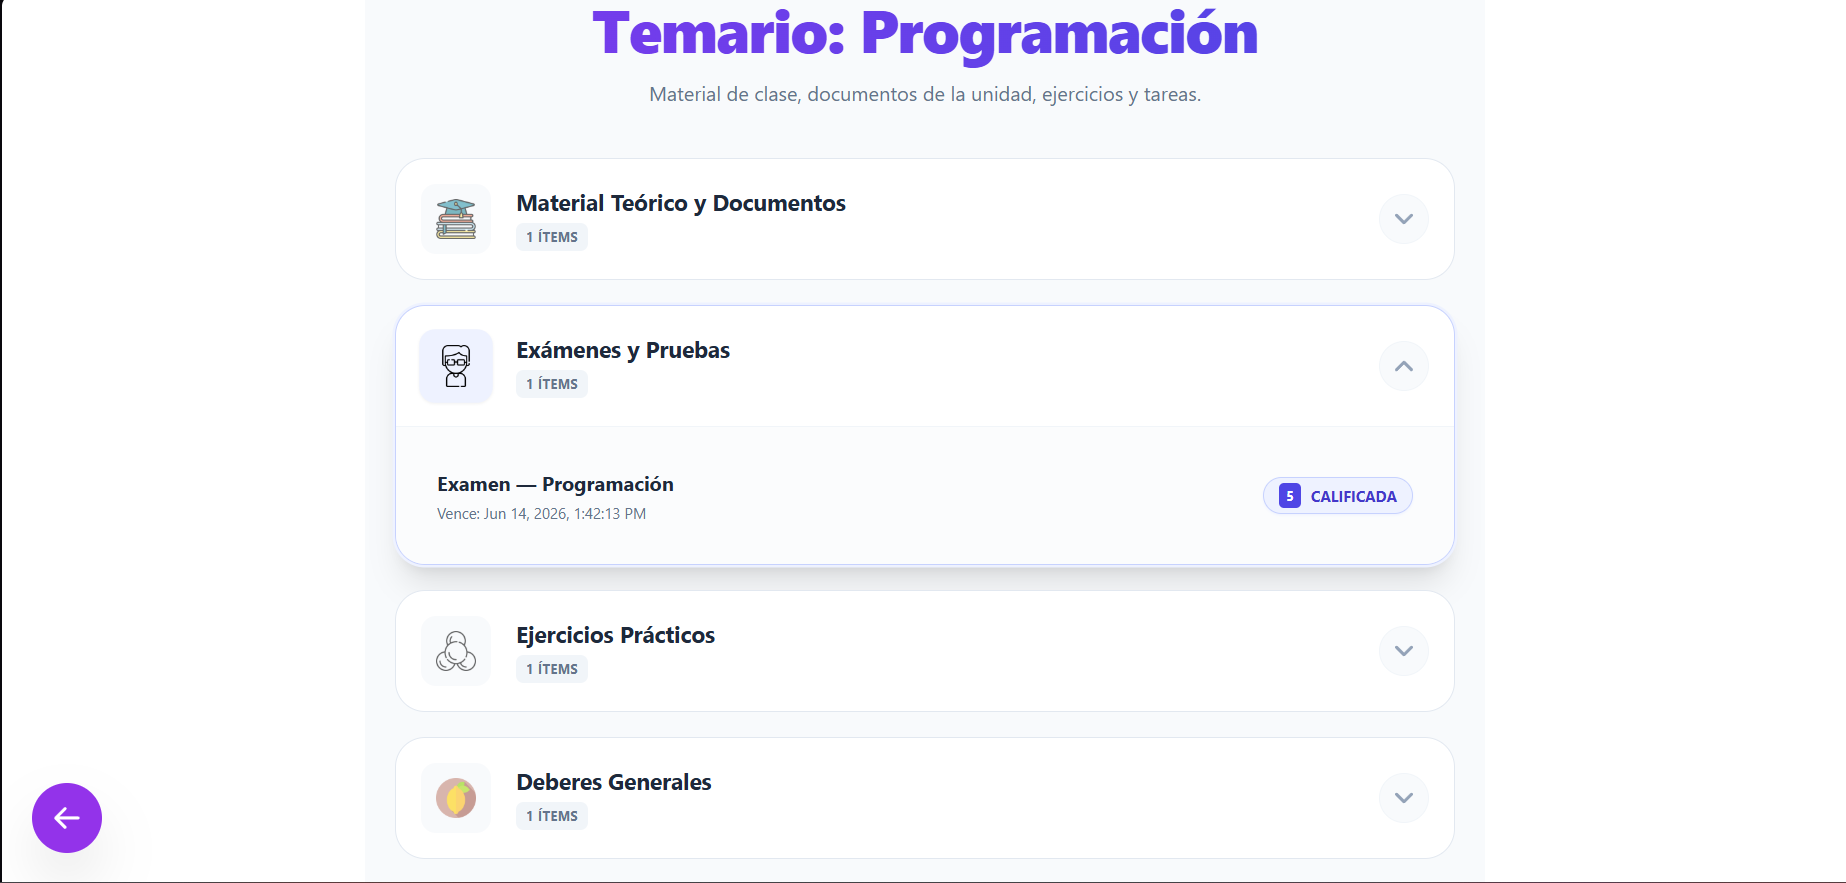
\includegraphics[keepaspectratio,alt={CAPTURA 8 --- Temario con bloques y tareas}]{../../assets/screenshots/manual-alumno/captura08-temario.png}}
\caption{CAPTURA 8 --- Temario con bloques y tareas}
\end{figure}

\subsection{7.2 Estados de una tarea (en el
listado)}\label{estados-de-una-tarea-en-el-listado}

{\def\LTcaptype{none} % do not increment counter
\begin{longtable}[]{@{}
  >{\raggedright\arraybackslash}p{(\linewidth - 2\tabcolsep) * \real{0.3810}}
  >{\raggedright\arraybackslash}p{(\linewidth - 2\tabcolsep) * \real{0.6190}}@{}}
\toprule\noalign{}
\begin{minipage}[b]{\linewidth}\raggedright
Estado
\end{minipage} & \begin{minipage}[b]{\linewidth}\raggedright
Significado
\end{minipage} \\
\midrule\noalign{}
\endhead
\bottomrule\noalign{}
\endlastfoot
\textbf{PENDIENTE} & Aún no has entregado (puede estar dentro o fuera de
plazo) \\
\textbf{ENTREGADA} & Has enviado tu trabajo; pendiente de corrección \\
\textbf{CALIFICADA} & El profesor ha puesto nota (se muestra la
puntuación) \\
\textbf{VENCIDA} & Plazo pasado sin entrega válida \\
\end{longtable}
}

\subsection{7.3 Abrir el detalle de una
tarea}\label{abrir-el-detalle-de-una-tarea}

\begin{enumerate}
\def\labelenumi{\arabic{enumi}.}
\tightlist
\item
  Pulsa sobre la fila de la tarea.
\item
  Se abre la pantalla de \textbf{detalle de tarea}
  (\texttt{/tarea/:id}).
\end{enumerate}

\begin{center}\rule{0.5\linewidth}{0.5pt}\end{center}

\section{8. Detalle de tarea: consulta, entrega y
nota}\label{detalle-de-tarea-consulta-entrega-y-nota}

\subsection{8.1 Información de la
tarea}\label{informaciuxf3n-de-la-tarea}

En la parte superior verás:

\begin{itemize}
\tightlist
\item
  \textbf{Título} y \textbf{estado} (badge de color)
\item
  \textbf{Fecha límite} de entrega
\item
  \textbf{Tipo} de tarea (deberes, práctica, examen, etc.)
\item
  \textbf{Descripción} del profesor
\item
  \textbf{Material de consulta}: enlace para ver o descargar el archivo
  adjunto del profesor (si existe)
\end{itemize}

\begin{figure}
\centering
\pandocbounded{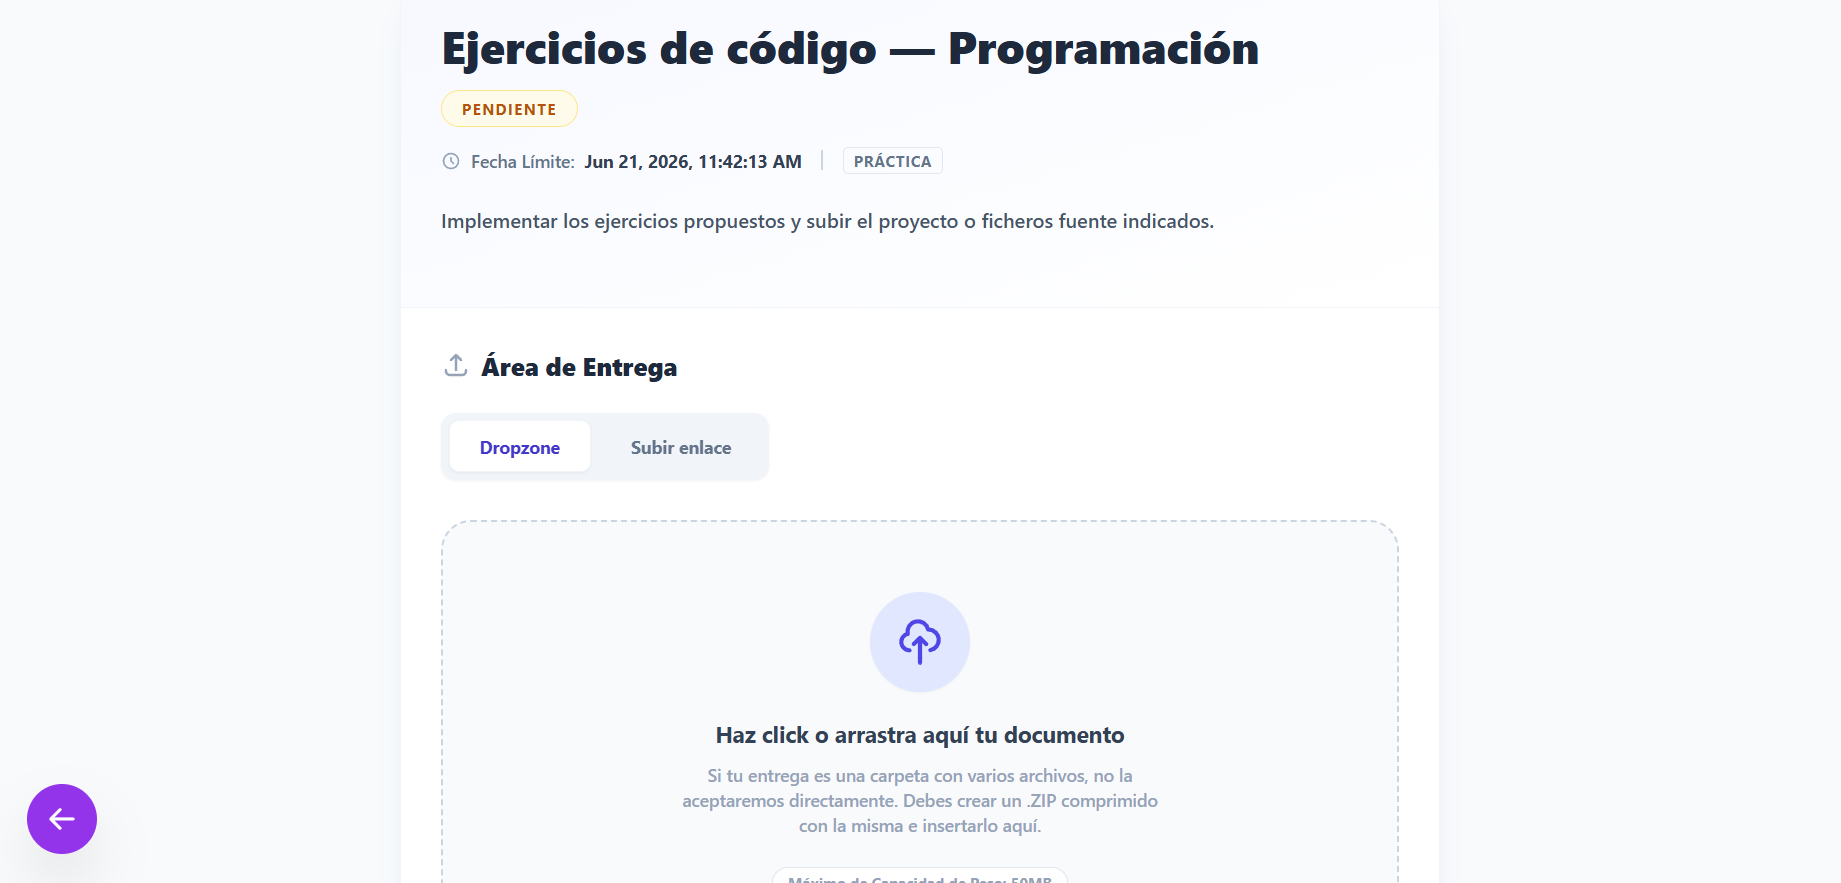
\includegraphics[keepaspectratio,alt={CAPTURA 9 --- Detalle de tarea}]{../../assets/screenshots/manual-alumno/captura09-detalle_tarea.png}}
\caption{CAPTURA 9 --- Detalle de tarea}
\end{figure}

\subsection{8.2 Si la tarea ya está
calificada}\label{si-la-tarea-ya-estuxe1-calificada}

Aparece la sección \textbf{Evaluación del profesor} con:

\begin{itemize}
\tightlist
\item
  \textbf{Nota final} (0--10)
\item
  \textbf{Comentarios} del profesor (si los hubo)
\end{itemize}

\begin{figure}
\centering
\pandocbounded{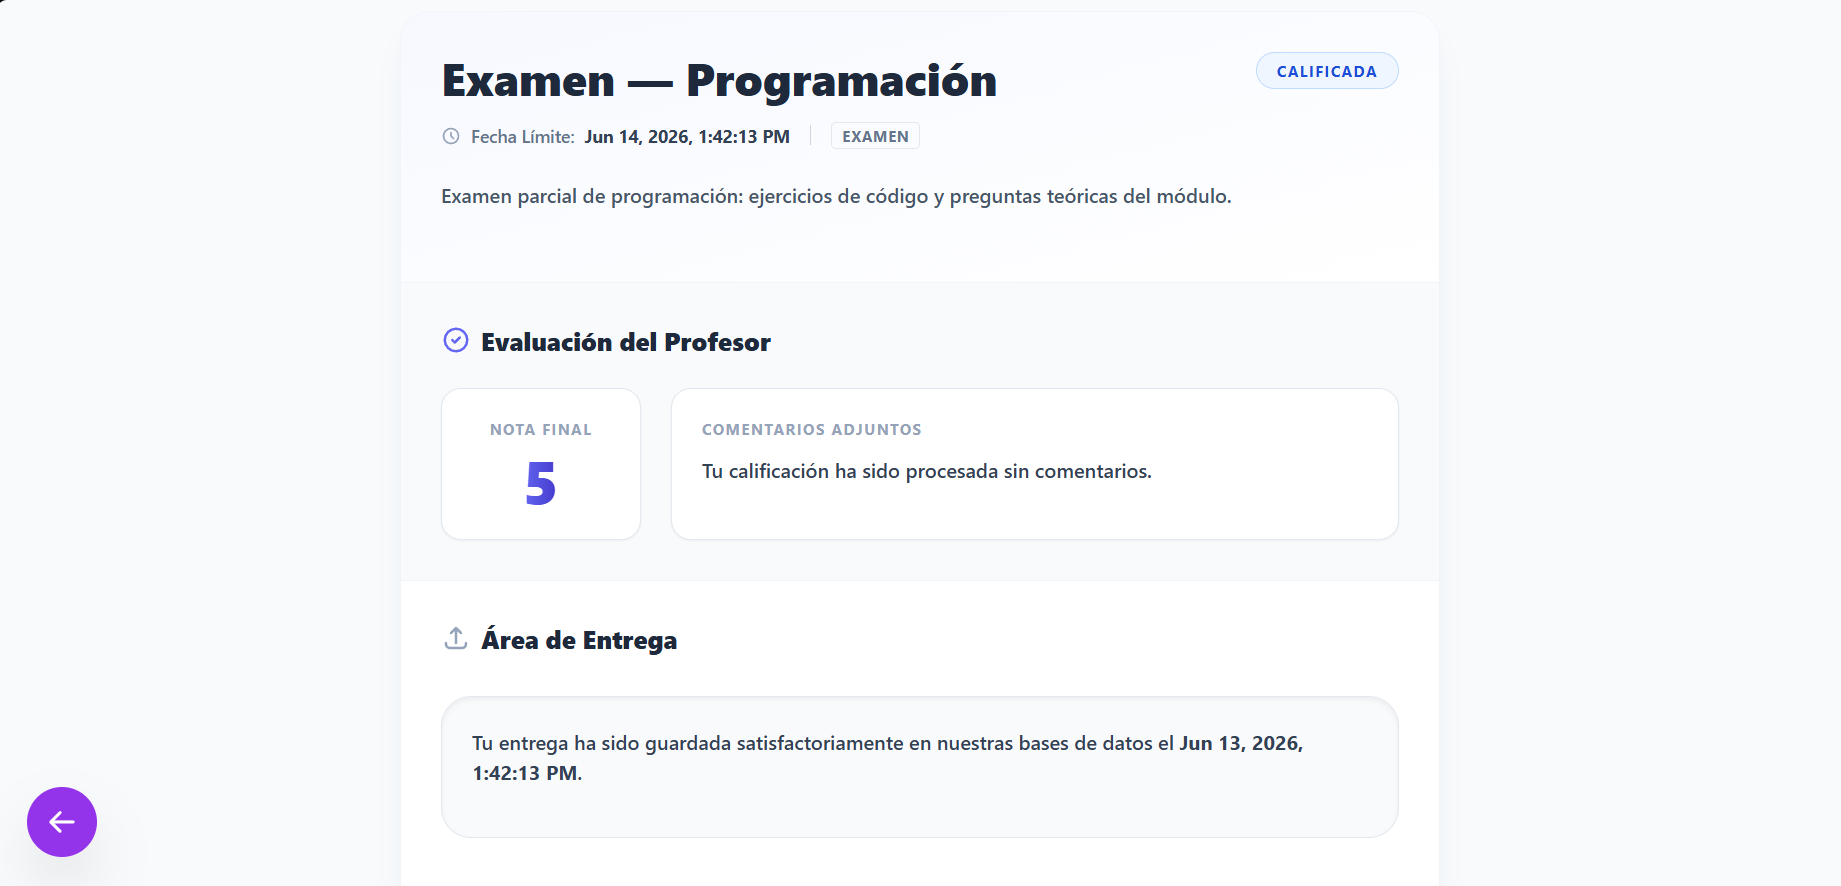
\includegraphics[keepaspectratio,alt={CAPTURA 10 --- Tarea entregada / evaluación del profesor}]{../../assets/screenshots/manual-alumno/captura10-tarea_entregada.png}}
\caption{CAPTURA 10 --- Tarea entregada / evaluación del profesor}
\end{figure}

\subsection{8.3 Entregar una tarea
(pendiente)}\label{entregar-una-tarea-pendiente}

En el \textbf{Área de entrega} puedes elegir dos modos:

\subsubsection{Modo A --- Subir archivo
(Dropzone)}\label{modo-a-subir-archivo-dropzone}

\begin{enumerate}
\def\labelenumi{\arabic{enumi}.}
\tightlist
\item
  Selecciona la pestaña de subida de archivo.
\item
  \textbf{Arrastra} un archivo a la zona punteada \textbf{o} haz clic
  para elegirlo en el explorador.
\item
  Formatos habituales: documentos, imágenes, ZIP (si son varios
  archivos, \textbf{comprime en .ZIP}).
\item
  Tamaño máximo indicado en pantalla: \textbf{50 MB}.
\item
  Tras seleccionar el archivo, revisa el nombre y pulsa
  \textbf{Confirmar envío al servidor}.
\end{enumerate}

\begin{figure}
\centering
\pandocbounded{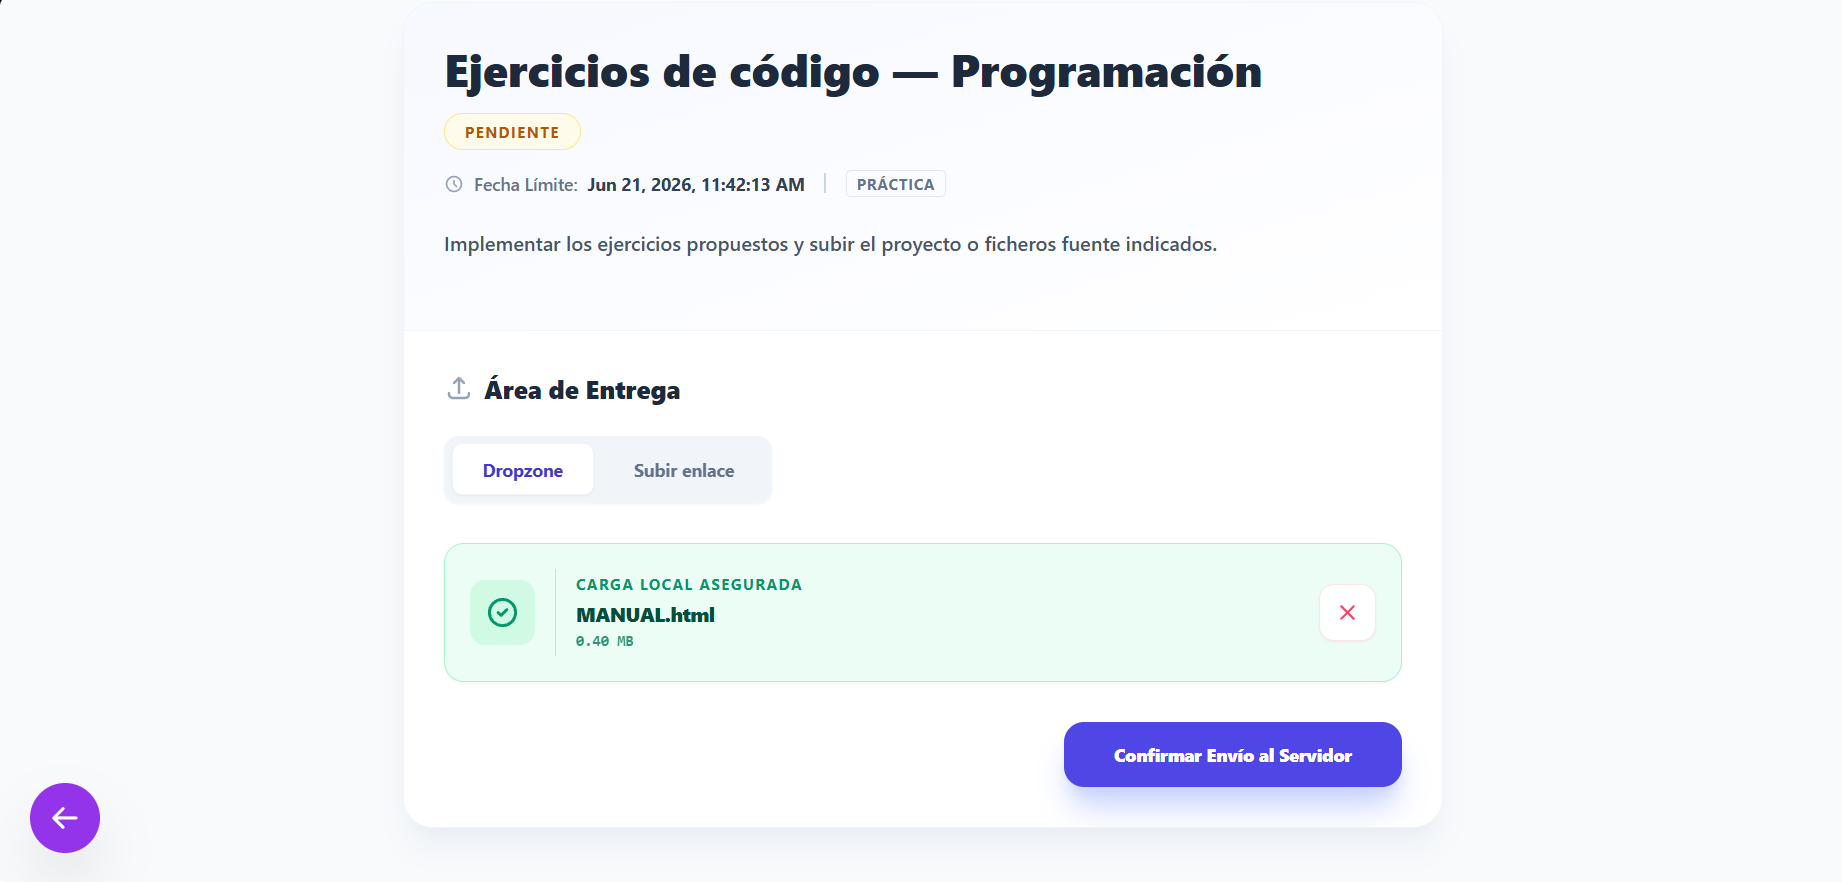
\includegraphics[keepaspectratio,alt={CAPTURA 11 --- Zona de arrastre con archivo seleccionado}]{../../assets/screenshots/manual-alumno/captura11-tarea_subida.png}}
\caption{CAPTURA 11 --- Zona de arrastre con archivo seleccionado}
\end{figure}

\subsubsection{Modo B --- Enlace URL}\label{modo-b-enlace-url}

\begin{enumerate}
\def\labelenumi{\arabic{enumi}.}
\tightlist
\item
  Cambia a la pestaña \textbf{Subir enlace}.
\item
  Introduce una URL válida (\texttt{http://} o \texttt{https://}), por
  ejemplo un Google Docs.
\item
  Pulsa \textbf{Confirmar envío al servidor}.
\end{enumerate}

\begin{figure}
\centering
\pandocbounded{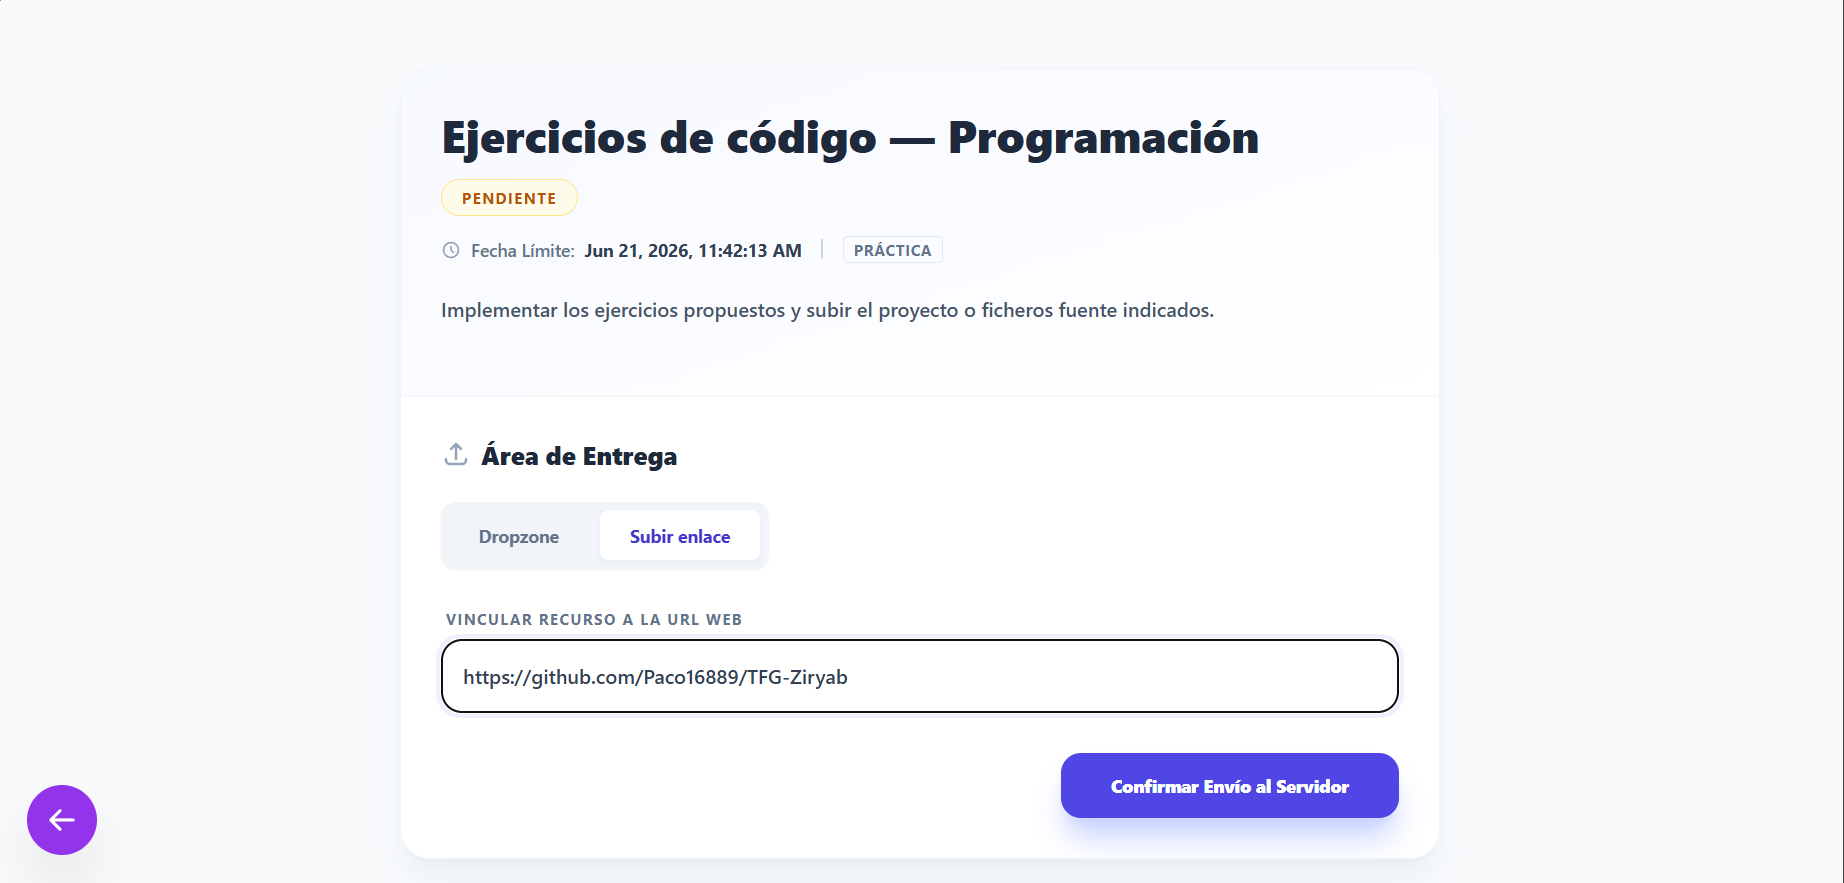
\includegraphics[keepaspectratio,alt={CAPTURA 12 --- Pestaña de enlace con URL rellenada}]{../../assets/screenshots/manual-alumno/captura12-enlace_entregado.png}}
\caption{CAPTURA 12 --- Pestaña de enlace con URL rellenada}
\end{figure}

\subsection{8.4 Avisos importantes al
entregar}\label{avisos-importantes-al-entregar}

\begin{itemize}
\tightlist
\item
  Si el plazo ha pasado pero el profesor \textbf{permite entrega
  tardía}, tu entrega puede quedar como \textbf{Retraso (LATE)}.
\item
  Si el plazo ha pasado y \textbf{no} se permiten entregas tardías,
  verás un aviso y \textbf{no podrás enviar}.
\item
  Tras un envío correcto aparece mensaje verde de confirmación.
\end{itemize}

\subsection{8.5 Modificar o borrar una
entrega}\label{modificar-o-borrar-una-entrega}

\begin{itemize}
\tightlist
\item
  Si ya entregaste y \textbf{aún no está calificada}, puedes usar
  \textbf{Borrar entrega} y volver a subir.
\item
  Si ya está \textbf{calificada}, no podrás eliminar la entrega desde
  esta pantalla.
\end{itemize}

\subsection{8.6 Errores frecuentes en la
entrega}\label{errores-frecuentes-en-la-entrega}

{\def\LTcaptype{none} % do not increment counter
\begin{longtable}[]{@{}ll@{}}
\toprule\noalign{}
Mensaje / situación & Qué hacer \\
\midrule\noalign{}
\endhead
\bottomrule\noalign{}
\endlastfoot
Carpeta no permitida & Comprime la carpeta en un archivo
\textbf{.ZIP} \\
Archivo demasiado grande & Reduce el tamaño por debajo de 50 MB \\
URL inválida & Comprueba que empiece por http:// o https:// \\
Error de servidor & Reintenta; si persiste, contacta con el profesor \\
\end{longtable}
}

\begin{center}\rule{0.5\linewidth}{0.5pt}\end{center}

\section{9. Gestión académica (menú
central)}\label{gestiuxf3n-acaduxe9mica-menuxfa-central}

Ruta: \textbf{Dashboard → Gestión} (\texttt{/gestion}).

Pantalla \textbf{Gestión académica} con acceso a cinco áreas:

{\def\LTcaptype{none} % do not increment counter
\begin{longtable}[]{@{}ll@{}}
\toprule\noalign{}
Tarjeta & Función \\
\midrule\noalign{}
\endhead
\bottomrule\noalign{}
\endlastfoot
\textbf{Ficha Usuario} & Historial de faltas y justificantes \\
\textbf{Horario} & Horario semanal de clases \\
\textbf{Calendario} & Calendario del centro (vista embebida) \\
\textbf{Tablón} & Anuncios / incidencias publicadas \\
\textbf{Evaluaciones} & Tus notas por trimestre \\
\end{longtable}
}

\begin{figure}
\centering
\pandocbounded{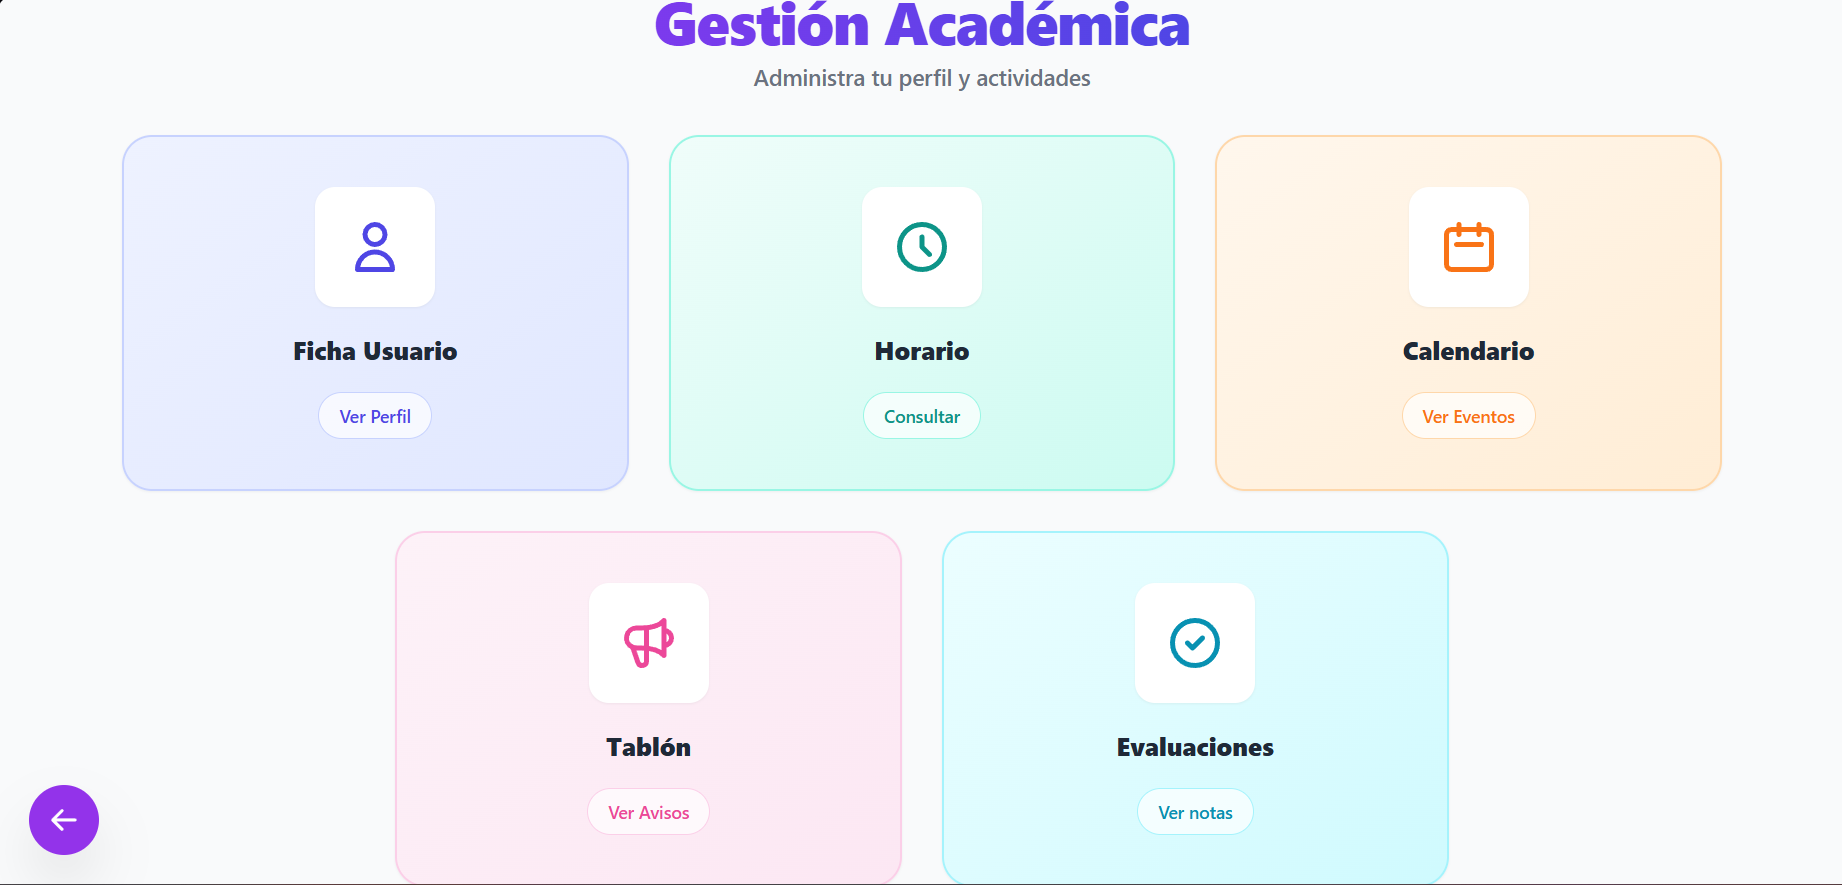
\includegraphics[keepaspectratio,alt={CAPTURA 13 --- Pantalla Gestión académica}]{../../assets/screenshots/manual-alumno/captura13-pantalla_gestion.png}}
\caption{CAPTURA 13 --- Pantalla Gestión académica}
\end{figure}

\begin{center}\rule{0.5\linewidth}{0.5pt}\end{center}

\section{10. Ficha de usuario y
asistencia}\label{ficha-de-usuario-y-asistencia}

Ruta: \textbf{Gestión → Ficha Usuario} (\texttt{/ficha-usuario}).

\subsection{10.1 Consultar faltas}\label{consultar-faltas}

\begin{itemize}
\tightlist
\item
  Listado de \textbf{faltas y retrasos} registrados por sesión.
\item
  Cada fila muestra: \textbf{asignatura}, \textbf{fecha}, \textbf{hora},
  \textbf{estado de asistencia} y \textbf{estado del justificante}.
\item
  Si no tienes faltas, verás un mensaje positivo indicando que no hay
  registros.
\end{itemize}

Estados de asistencia:

{\def\LTcaptype{none} % do not increment counter
\begin{longtable}[]{@{}ll@{}}
\toprule\noalign{}
Etiqueta & Significado \\
\midrule\noalign{}
\endhead
\bottomrule\noalign{}
\endlastfoot
FALTA & Ausencia \\
RETRASO & Llegada tarde \\
JUSTIFICADA & Falta excusada oficialmente \\
\end{longtable}
}

\begin{figure}
\centering
\pandocbounded{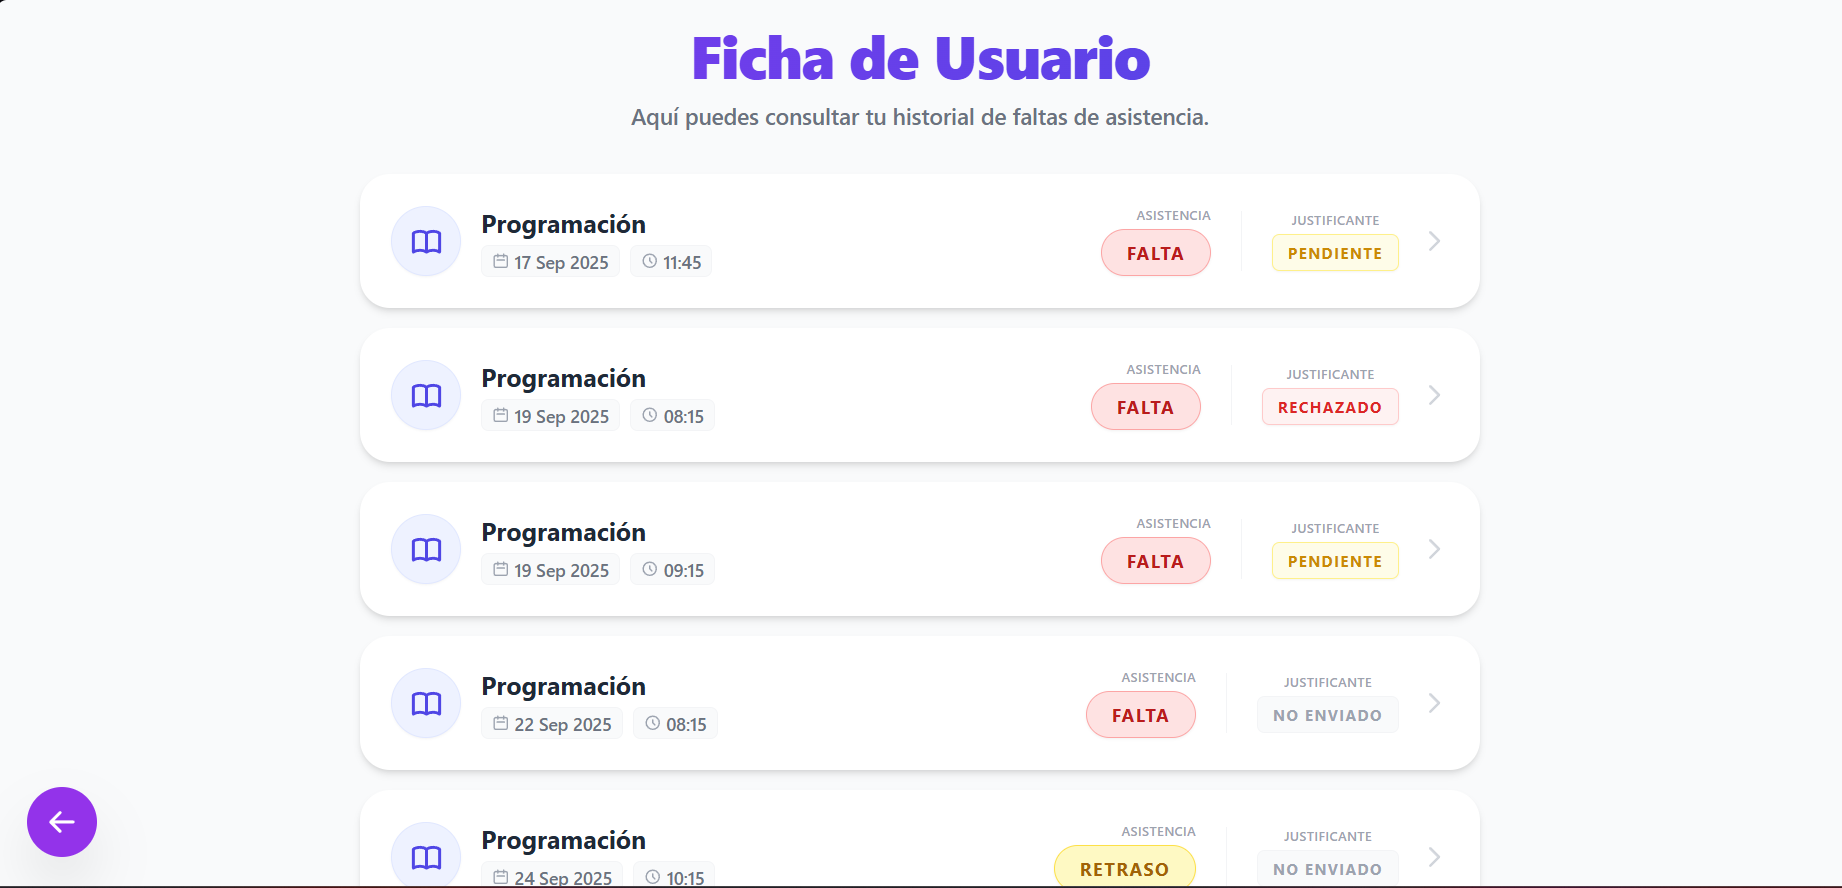
\includegraphics[keepaspectratio,alt={CAPTURA 14 --- Listado de faltas}]{../../assets/screenshots/manual-alumno/captura14-ficha_usuario.png}}
\caption{CAPTURA 14 --- Listado de faltas}
\end{figure}

\subsection{10.2 Justificar una falta}\label{justificar-una-falta}

\begin{enumerate}
\def\labelenumi{\arabic{enumi}.}
\tightlist
\item
  Pulsa sobre una falta que \textbf{no} esté ya justificada (filas
  interactivas).
\item
  Se abre el modal \textbf{Justificar falta}.
\item
  Selecciona un documento: \textbf{PNG, JPG o PDF}, máximo \textbf{1
  MB}.
\item
  Pulsa \textbf{Subir justificante}.
\item
  El estado pasará a \textbf{PENDIENTE} hasta que el profesor lo revise.
\end{enumerate}

\begin{figure}
\centering
\pandocbounded{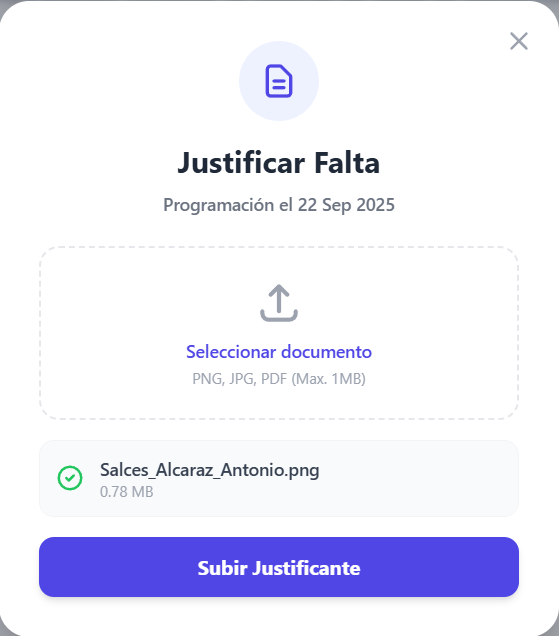
\includegraphics[keepaspectratio,alt={CAPTURA 15 --- Modal de justificación}]{../../assets/screenshots/manual-alumno/captura15-modal_justificar_falta.png}}
\caption{CAPTURA 15 --- Modal de justificación}
\end{figure}

\begin{figure}
\centering
\pandocbounded{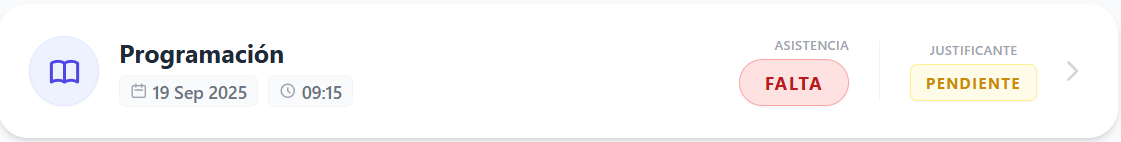
\includegraphics[keepaspectratio,alt={CAPTURA 16 --- Falta con justificante PENDIENTE}]{../../assets/screenshots/manual-alumno/captura16-justificacion_pendiente.png}}
\caption{CAPTURA 16 --- Falta con justificante PENDIENTE}
\end{figure}

Estados del justificante: \textbf{NO ENVIADO}, \textbf{PENDIENTE},
\textbf{ACEPTADO}, \textbf{RECHAZADO}.

\begin{center}\rule{0.5\linewidth}{0.5pt}\end{center}

\section{11. Horario semanal}\label{horario-semanal}

Ruta: \textbf{Gestión → Horario} (\texttt{/horario-alumno}).

\begin{itemize}
\tightlist
\item
  Vista en \textbf{columnas por día de la semana} (lunes a viernes o
  según configuración del centro).
\item
  En cada día aparecen las franjas con \textbf{hora inicio--fin} y
  \textbf{nombre de la asignatura}.
\item
  Si un día no tienes clase, verás un mensaje de día sin clases.
\end{itemize}

\begin{figure}
\centering
\pandocbounded{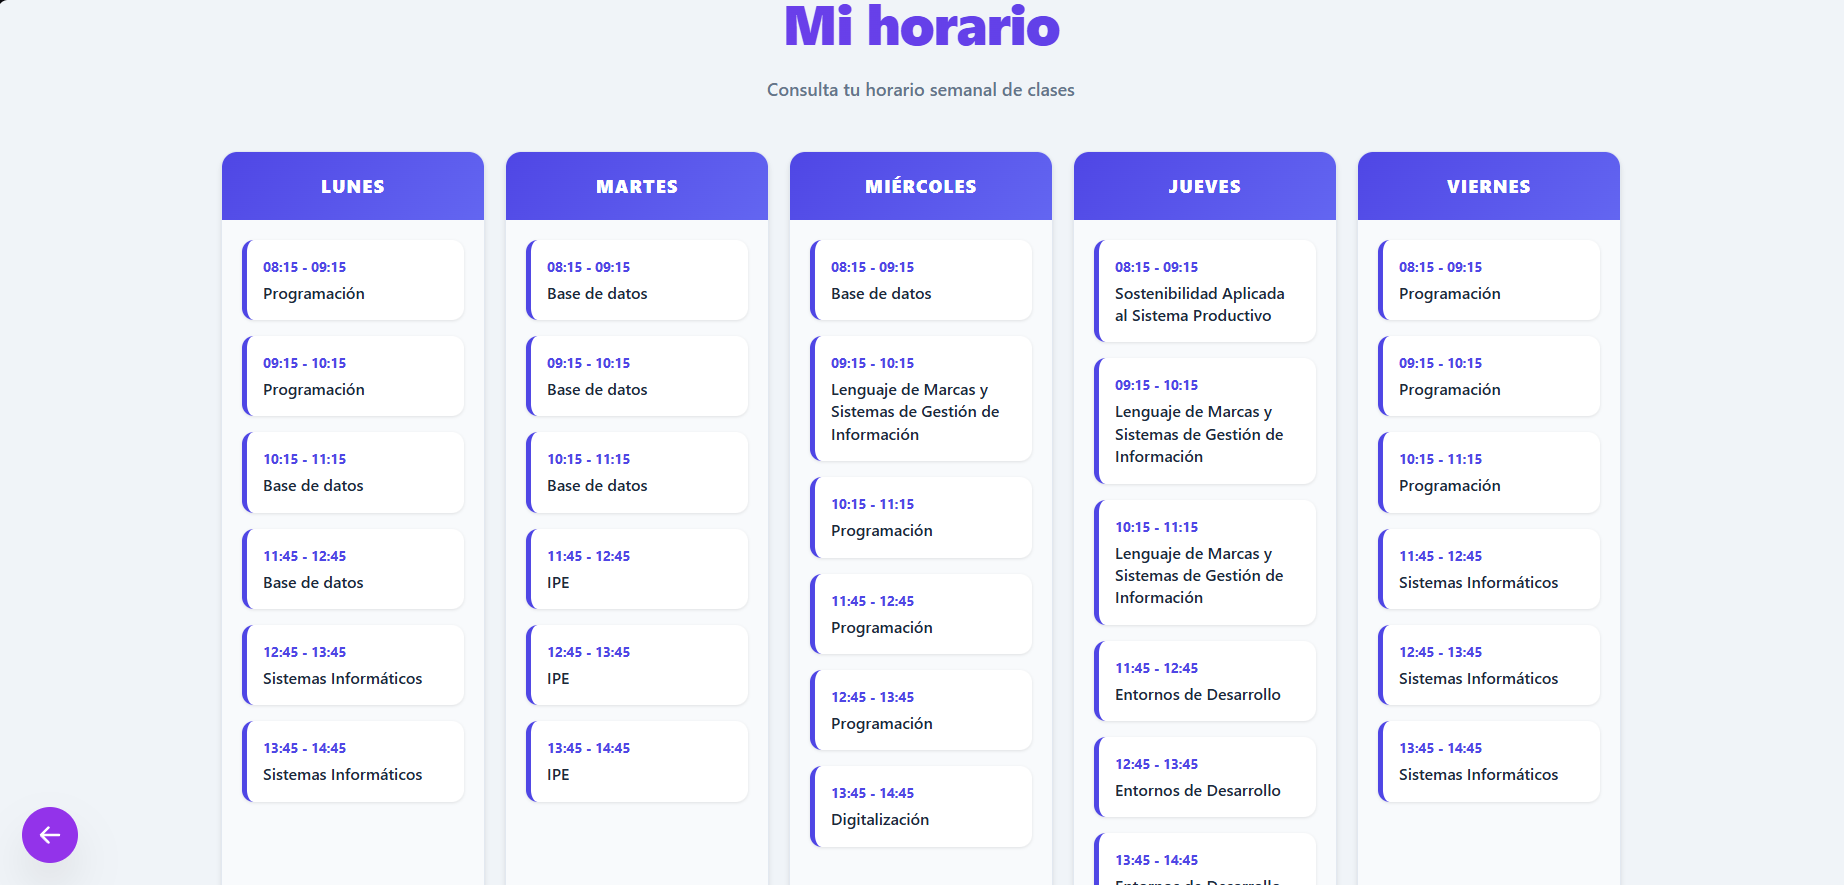
\includegraphics[keepaspectratio,alt={CAPTURA 17 --- Horario semanal del alumno}]{../../assets/screenshots/manual-alumno/captura17-horario.png}}
\caption{CAPTURA 17 --- Horario semanal del alumno}
\end{figure}

\begin{center}\rule{0.5\linewidth}{0.5pt}\end{center}

\section{12. Calendario}\label{calendario}

Ruta: \textbf{Gestión → Calendario} (\texttt{/calendario}).

\begin{itemize}
\tightlist
\item
  Muestra un \textbf{calendario embebido} (iframe) con eventos del
  centro.
\item
  Desplázate y navega dentro del calendario como en la herramienta
  externa configurada.
\end{itemize}

\begin{figure}
\centering
\pandocbounded{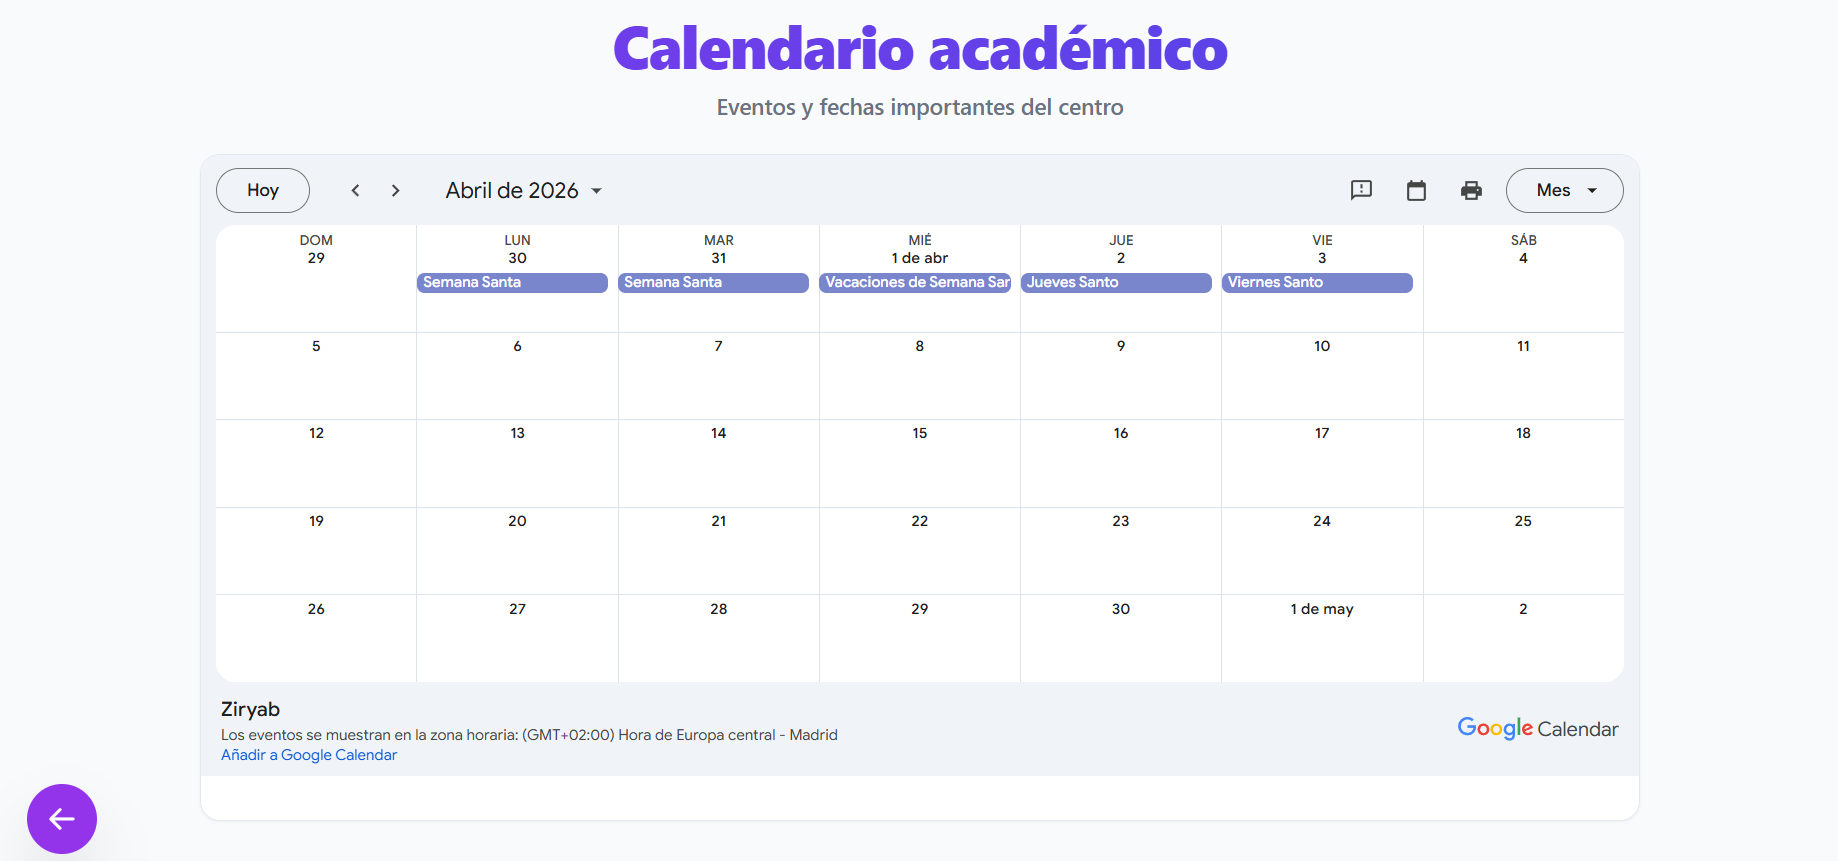
\includegraphics[keepaspectratio,alt={CAPTURA 18 --- Pantalla Calendario}]{../../assets/screenshots/manual-alumno/captura18-calendario.png}}
\caption{CAPTURA 18 --- Pantalla Calendario}
\end{figure}

\begin{center}\rule{0.5\linewidth}{0.5pt}\end{center}

\section{13. Tablón de anuncios}\label{tabluxf3n-de-anuncios}

Ruta: \textbf{Gestión → Tablón} (\texttt{/issues}).

\begin{itemize}
\tightlist
\item
  Listado de \textbf{anuncios} publicados para la comunidad educativa.
\item
  Consulta título, contenido y fecha de cada aviso (según diseño de la
  lista).
\end{itemize}

\begin{figure}
\centering
\pandocbounded{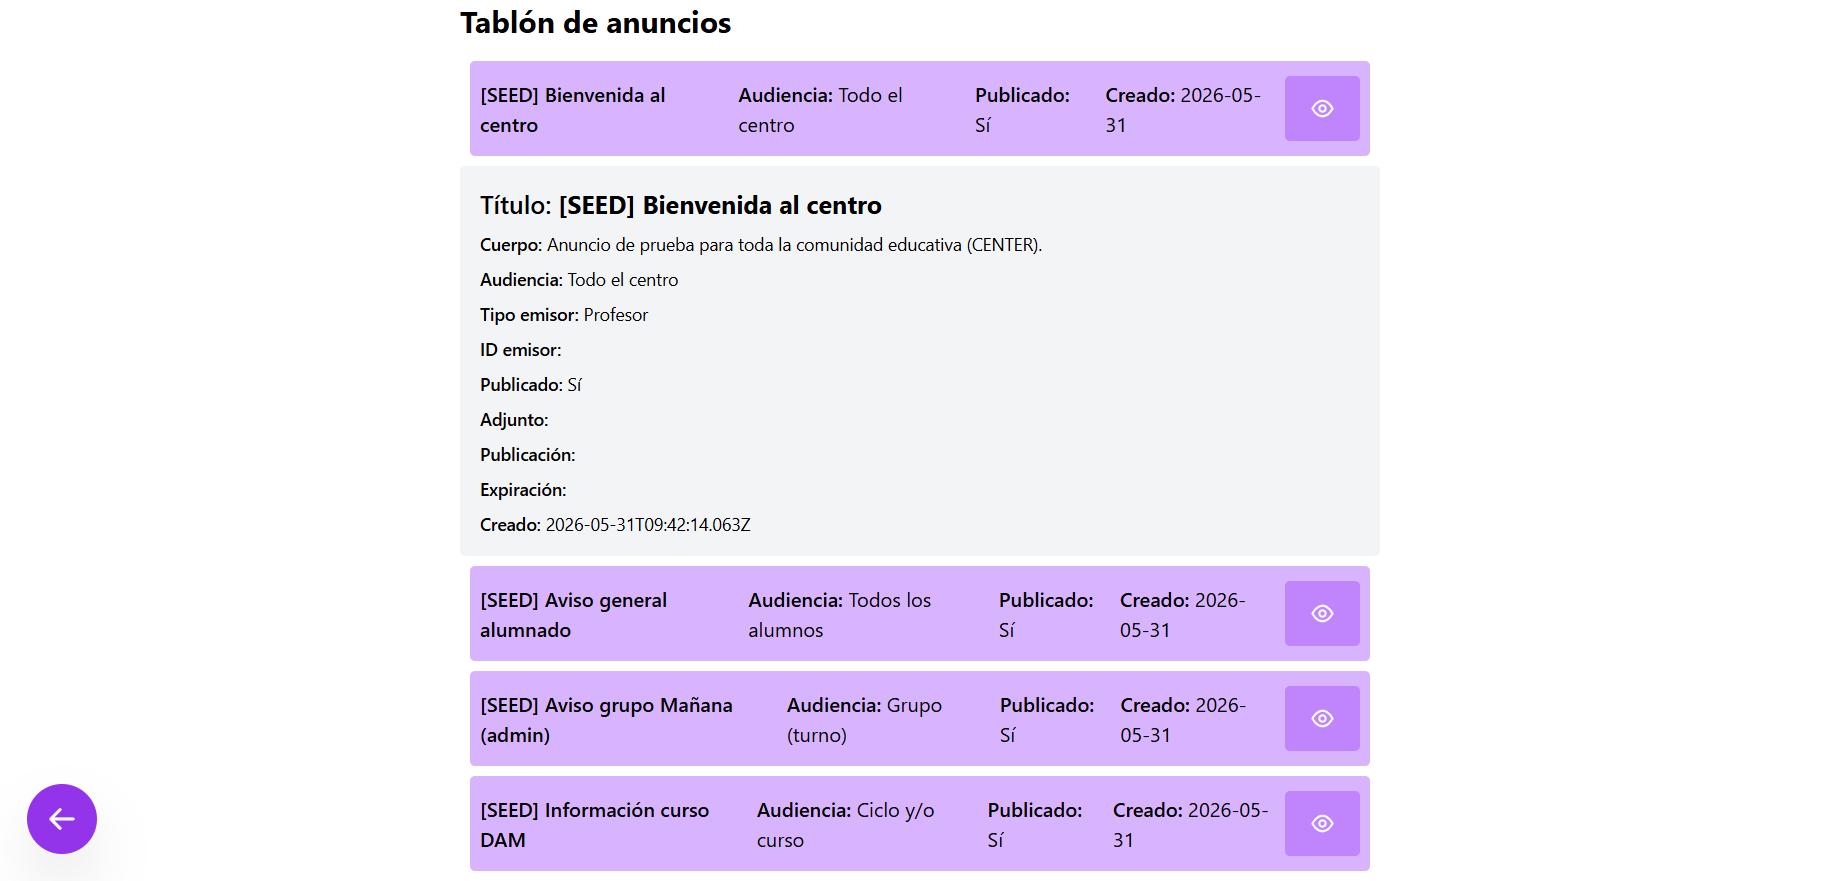
\includegraphics[keepaspectratio,alt={CAPTURA 19 --- Tablón de anuncios}]{../../assets/screenshots/manual-alumno/captura19-tablon.png}}
\caption{CAPTURA 19 --- Tablón de anuncios}
\end{figure}

\begin{center}\rule{0.5\linewidth}{0.5pt}\end{center}

\section{14. Mis evaluaciones (notas)}\label{mis-evaluaciones-notas}

Ruta: \textbf{Gestión → Evaluaciones} (\texttt{/mis-evaluaciones}).

\subsection{14.1 Tabla de calificaciones}\label{tabla-de-calificaciones}

\begin{itemize}
\tightlist
\item
  Tabla con \textbf{filas = asignaturas} y \textbf{columnas = periodos}
  de evaluación:

  \begin{itemize}
  \tightlist
  \item
    Evaluación inicial\\
  \item
    1º, 2º y 3º trimestre\\
  \item
    Nota final\\
  \end{itemize}
\item
  Las notas \textbf{inferiores a 5} suelen mostrarse en rojo; las
  aprobadas en verde.
\item
  La última fila muestra la \textbf{nota media} por periodo.
\end{itemize}

\begin{figure}
\centering
\pandocbounded{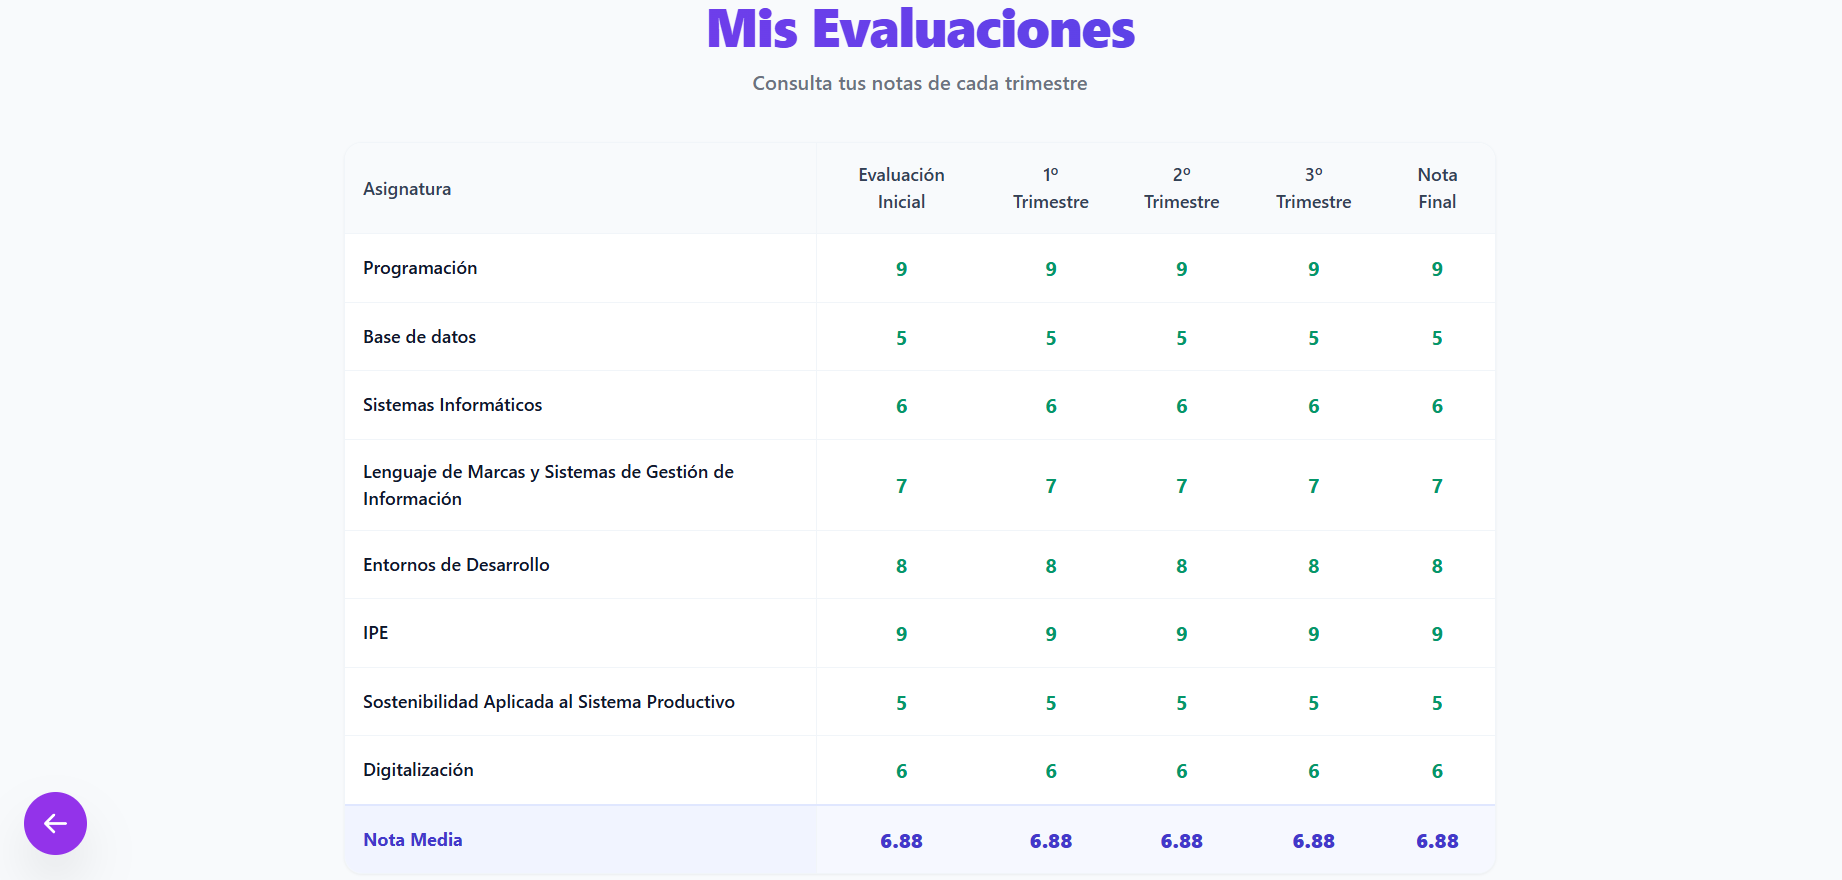
\includegraphics[keepaspectratio,alt={CAPTURA 20 --- Tabla de Mis evaluaciones}]{../../assets/screenshots/manual-alumno/captura20-evaluaciones.png}}
\caption{CAPTURA 20 --- Tabla de Mis evaluaciones}
\end{figure}

\subsection{14.2 Sin calificaciones}\label{sin-calificaciones}

Si el tutor o profesores aún no han introducido notas, verás: \emph{«Aún
no tienes calificaciones registradas»}.

\begin{center}\rule{0.5\linewidth}{0.5pt}\end{center}

\section{15. Flujo de trabajo recomendado
(resumen)}\label{flujo-de-trabajo-recomendado-resumen}

\begin{Shaded}
\begin{Highlighting}[]
\NormalTok{Login → Mi Espacio → Clases → Temario → Tarea → Entregar}
\NormalTok{                  ↘ Gestión → Ficha / Horario / Calendario / Tablón / Evaluaciones}
\end{Highlighting}
\end{Shaded}

\begin{center}\rule{0.5\linewidth}{0.5pt}\end{center}

\section{16. Preguntas frecuentes (FAQ)}\label{preguntas-frecuentes-faq}

\textbf{¿Puedo usar la app en el móvil?}\\
Sí; la interfaz es responsive, aunque algunas tablas se desplazan
horizontalmente.

\textbf{No veo ninguna asignatura}\\
Tu matrícula puede no estar activa; contacta con secretaría o
administración.

\textbf{He entregado pero sigue en PENDIENTE}\\
Comprueba que recibiste el mensaje de éxito; refresca la página. Si
persiste, avisa al profesor.

\textbf{Mi justificante fue rechazado}\\
Sube un nuevo documento válido o consulta con el profesor el motivo.

\textbf{¿Cómo cambio el idioma?}\\
Selector en la esquina superior izquierda de la cabecera.

\begin{center}\rule{0.5\linewidth}{0.5pt}\end{center}

\section{17. Glosario}\label{glosario}

{\def\LTcaptype{none} % do not increment counter
\begin{longtable}[]{@{}ll@{}}
\toprule\noalign{}
Término & Definición \\
\midrule\noalign{}
\endhead
\bottomrule\noalign{}
\endlastfoot
Temario & Conjunto de bloques y tareas de una asignatura \\
Entrega & Archivo o enlace que envías para una tarea \\
Trimestre & Periodo de evaluación académica \\
Justificante & Documento que acredita una ausencia \\
Tablón & Murales de avisos del centro \\
\end{longtable}
}

\begin{center}\rule{0.5\linewidth}{0.5pt}\end{center}

\emph{Fin del manual de alumno. Para incidencias técnicas, contacta con
el administrador del centro.}

\newpage

\chapter{Parte III --- Manual de usuario:
Profesor}\label{parte-iii-manual-de-usuario-profesor}

\textbf{Versión:} 1.0 · \textbf{Aplicación:} Ziryab --- Plataforma
Educativa\\
\textbf{Rol:} Profesor (TEACHER)\\
\textbf{Última actualización:} junio 2026 · \textbf{Capturas:} incluidas
(26 y 27 pendientes)

\begin{center}\rule{0.5\linewidth}{0.5pt}\end{center}

\section{1. Introducción}\label{introducciuxf3n-1}

\textbf{Ziryab} permite al profesorado gestionar sus asignaturas: crear
tareas, revisar entregas, calificar, pasar lista, validar justificantes
de ausencia y, si actúas como \textbf{tutor/a de grupo}, registrar las
evaluaciones trimestrales de tus alumnos.

Este manual cubre \textbf{todas las funcionalidades del rol TEACHER}.

\begin{center}\rule{0.5\linewidth}{0.5pt}\end{center}

\section{2. Requisitos previos}\label{requisitos-previos-1}

{\def\LTcaptype{none} % do not increment counter
\begin{longtable}[]{@{}
  >{\raggedright\arraybackslash}p{(\linewidth - 2\tabcolsep) * \real{0.5500}}
  >{\raggedright\arraybackslash}p{(\linewidth - 2\tabcolsep) * \real{0.4500}}@{}}
\toprule\noalign{}
\begin{minipage}[b]{\linewidth}\raggedright
Requisito
\end{minipage} & \begin{minipage}[b]{\linewidth}\raggedright
Detalle
\end{minipage} \\
\midrule\noalign{}
\endhead
\bottomrule\noalign{}
\endlastfoot
Navegador & Chrome, Firefox, Edge o Safari actualizado \\
Credenciales & Cuenta de profesor con asignaturas asignadas en el
sistema \\
Rol tutor (opcional) & Necesario para la pantalla \textbf{Evaluaciones}
de grupo tutorizado \\
Idiomas & ES / EN / DE desde la cabecera \\
\end{longtable}
}

\begin{center}\rule{0.5\linewidth}{0.5pt}\end{center}

\section{3. Inicio de sesión}\label{inicio-de-sesiuxf3n-1}

El acceso es idéntico al del alumno:

\begin{enumerate}
\def\labelenumi{\arabic{enumi}.}
\tightlist
\item
  Abre la URL de Ziryab.
\item
  Introduce \textbf{email} y \textbf{contraseña}.
\item
  Pulsa el botón de acceso.
\end{enumerate}

\begin{figure}
\centering
\pandocbounded{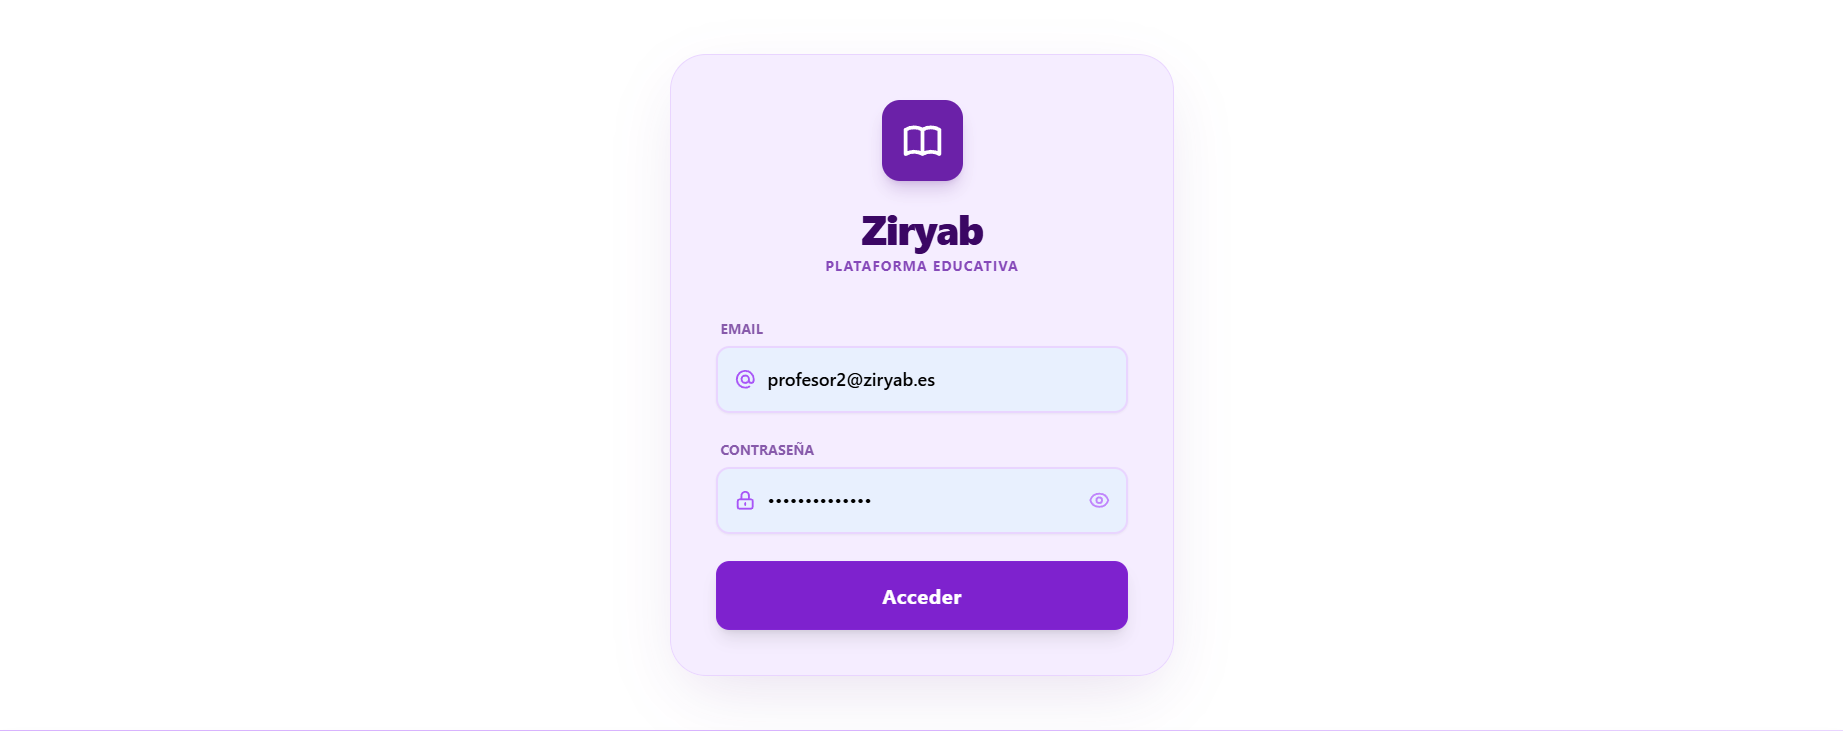
\includegraphics[keepaspectratio,alt={CAPTURA 1 --- Pantalla de login}]{../../assets/screenshots/manual-profesor/captura1-login.png}}
\caption{CAPTURA 1 --- Pantalla de login}
\end{figure}

Tras un login correcto con rol \textbf{TEACHER}, entrarás al
\textbf{Dashboard (Mi Espacio)} con las mismas dos tarjetas principales,
pero la tarjeta \textbf{Clases} te llevará a \textbf{Mis clases} del
profesor.

\begin{center}\rule{0.5\linewidth}{0.5pt}\end{center}

\section{4. Interfaz general
(cabecera)}\label{interfaz-general-cabecera-1}

La cabecera morada incluye:

{\def\LTcaptype{none} % do not increment counter
\begin{longtable}[]{@{}ll@{}}
\toprule\noalign{}
Elemento & Función \\
\midrule\noalign{}
\endhead
\bottomrule\noalign{}
\endlastfoot
Selector de idioma & Cambia el idioma de la interfaz \\
\textbf{Ziryab} (centro) & Vuelve al Dashboard \\
Notificaciones & Avisos de entregas, justificantes, etc. \\
Perfil (nombre + «PROFESOR») & Menú con \textbf{Cerrar sesión} \\
\end{longtable}
}

\begin{figure}
\centering
\pandocbounded{
\includegraphics[keepaspectratio,alt={CAPTURA 2 --- Cabecera con rol Profesor visible}]{../../assets/screenshots/manual-profesor/captura2-cabecera.png}}
\caption{CAPTURA 2 --- Cabecera con rol Profesor visible}
\end{figure}

\subsection{4.1 Notificaciones y cierre de
sesión}\label{notificaciones-y-cierre-de-sesiuxf3n}

\begin{itemize}
\tightlist
\item
  \textbf{Campana:} abre el listado de notificaciones; puedes marcarlas
  como leídas.
\item
  \textbf{Perfil → Cerrar sesión:} finaliza la sesión de forma segura.
\end{itemize}

\begin{figure}
\centering
\pandocbounded{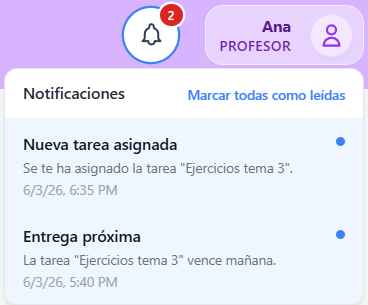
\includegraphics[keepaspectratio,alt={CAPTURA 3 --- Panel de notificaciones}]{../../assets/screenshots/manual-profesor/captura3-notificaciones.png}}
\caption{CAPTURA 3 --- Panel de notificaciones}
\end{figure}

\begin{figure}
\centering
\pandocbounded{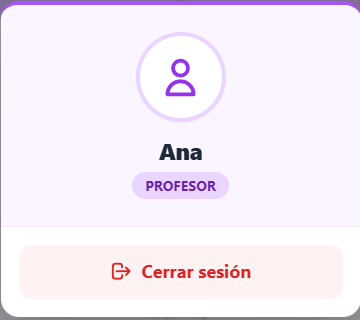
\includegraphics[keepaspectratio,alt={CAPTURA 4 --- Modal de perfil}]{../../assets/screenshots/manual-profesor/captura4-modal.png}}
\caption{CAPTURA 4 --- Modal de perfil}
\end{figure}

\begin{center}\rule{0.5\linewidth}{0.5pt}\end{center}

\section{5. Panel principal --- «Mi
Espacio»}\label{panel-principal-mi-espacio}

Pantalla inicial con dos accesos:

{\def\LTcaptype{none} % do not increment counter
\begin{longtable}[]{@{}
  >{\raggedright\arraybackslash}p{(\linewidth - 2\tabcolsep) * \real{0.3214}}
  >{\raggedright\arraybackslash}p{(\linewidth - 2\tabcolsep) * \real{0.6786}}@{}}
\toprule\noalign{}
\begin{minipage}[b]{\linewidth}\raggedright
Tarjeta
\end{minipage} & \begin{minipage}[b]{\linewidth}\raggedright
Destino (profesor)
\end{minipage} \\
\midrule\noalign{}
\endhead
\bottomrule\noalign{}
\endlastfoot
\textbf{Clases} & \texttt{/clases-profesor} --- Asignaturas que
impartes \\
\textbf{Gestión} & \texttt{/gestion} --- Ficha, horario, calendario,
tablón, evaluaciones \\
\end{longtable}
}

\begin{figure}
\centering
\pandocbounded{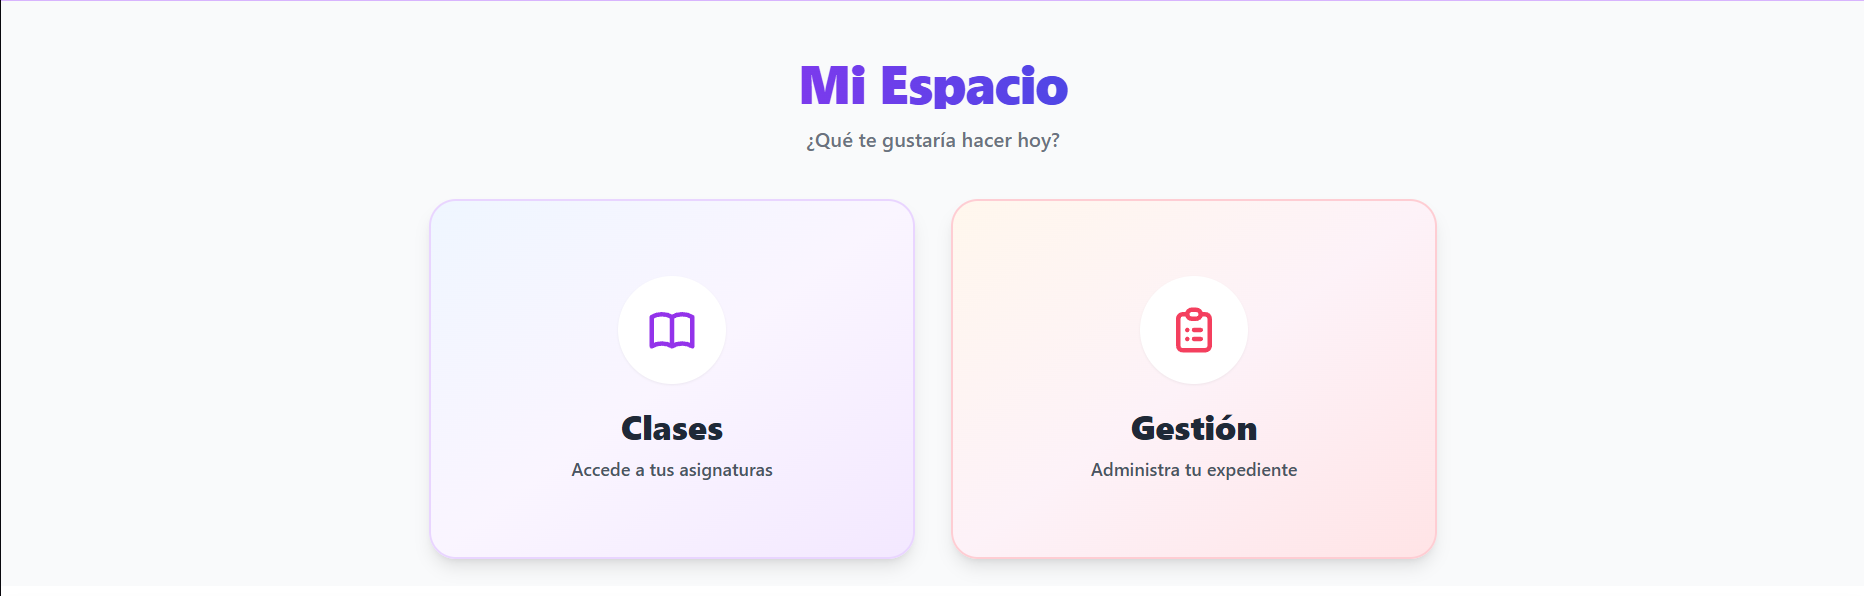
\includegraphics[keepaspectratio,alt={CAPTURA 5 --- Dashboard del profesor}]{../../assets/screenshots/manual-profesor/captura5-dashboard.png}}
\caption{CAPTURA 5 --- Dashboard del profesor}
\end{figure}

\begin{center}\rule{0.5\linewidth}{0.5pt}\end{center}

\section{6. Mis clases (asignaturas
asignadas)}\label{mis-clases-asignaturas-asignadas}

Ruta: \textbf{Mi Espacio → Clases} (\texttt{/clases-profesor}).

\subsection{6.1 Listado}\label{listado}

Cada tarjeta representa una \textbf{asignación} (asignatura + grupo +
ciclo) y muestra:

\begin{itemize}
\tightlist
\item
  Nombre de la \textbf{asignatura}
\item
  \textbf{Ciclo} y \textbf{grupo}
\item
  Dos acciones:

  \begin{enumerate}
  \def\labelenumi{\arabic{enumi}.}
  \tightlist
  \item
    \textbf{Gestionar temario} --- Material, tareas y asistencia de esa
    asignatura
  \item
    \textbf{Menú de clase} --- Acceso rápido a tareas y justificaciones
  \end{enumerate}
\end{itemize}

\begin{figure}
\centering
\pandocbounded{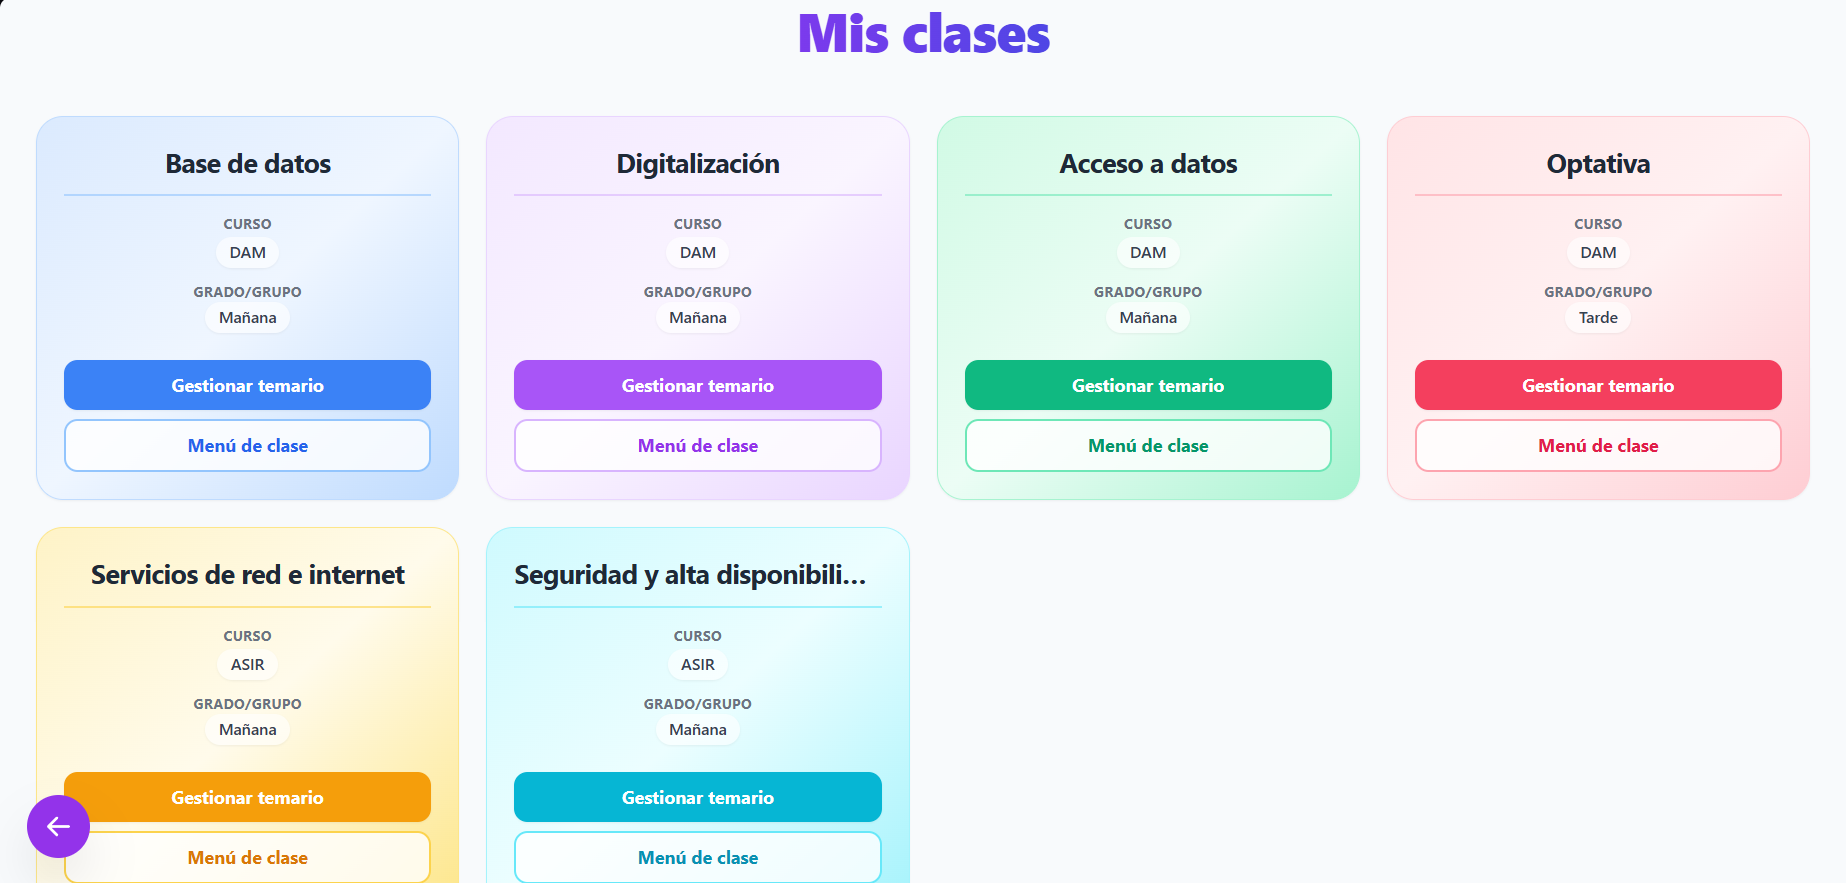
\includegraphics[keepaspectratio,alt={CAPTURA 6 --- Listado «Mis clases» con dos botones por tarjeta}]{../../assets/screenshots/manual-profesor/captura6-clases.png}}
\caption{CAPTURA 6 --- Listado «Mis clases» con dos botones por tarjeta}
\end{figure}

\subsection{6.2 Sin asignaturas}\label{sin-asignaturas}

Si no tienes asignaturas asignadas, verás un mensaje informativo.
Contacta con administración para revisar tu carga docente en el sistema.

\begin{center}\rule{0.5\linewidth}{0.5pt}\end{center}

\section{7. Programación / Temario del
profesor}\label{programaciuxf3n-temario-del-profesor}

Ruta: \textbf{Gestionar temario} → \texttt{/temario-profesor/:claseId}

\subsection{7.1 Vista general}\label{vista-general}

\begin{itemize}
\tightlist
\item
  Título \textbf{Programación}.
\item
  Botón \textbf{Pasar lista} (esquina superior derecha): abre el modal
  de asistencia.
\item
  Bloques por tipo de contenido (teoría, exámenes, proyectos, prácticas,
  deberes), igual que ve el alumno pero con \textbf{controles de
  profesor}.
\end{itemize}

\begin{figure}
\centering
\pandocbounded{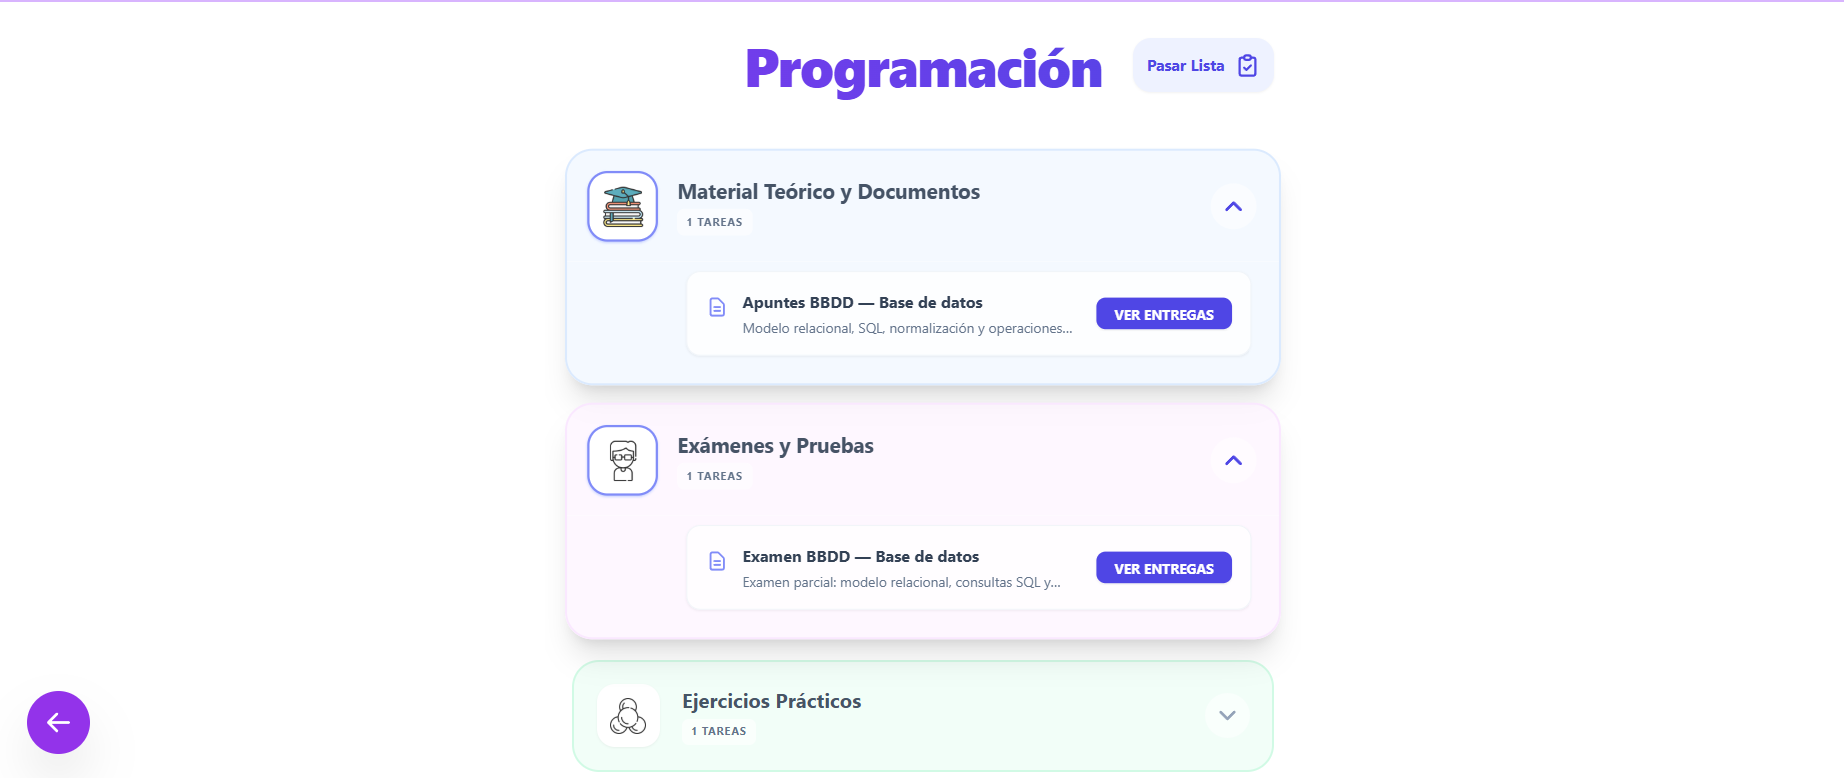
\includegraphics[keepaspectratio,alt={CAPTURA 7 --- Temario del profesor con botón Pasar lista}]{../../assets/screenshots/manual-profesor/captura8-temario.png}}
\caption{CAPTURA 7 --- Temario del profesor con botón Pasar lista}
\end{figure}

\subsection{7.2 Gestionar tareas dentro del
temario}\label{gestionar-tareas-dentro-del-temario}

En cada bloque expandido, cada tarea muestra:

\begin{itemize}
\tightlist
\item
  Título y descripción
\item
  \textbf{Ver archivo base} --- Abre el adjunto que subiste al crear la
  tarea
\item
  \textbf{Ver entregas} --- Ir al listado de entregas de los alumnos
\end{itemize}

\subsection{7.3 Pasar lista (asistencia)}\label{pasar-lista-asistencia}

\begin{enumerate}
\def\labelenumi{\arabic{enumi}.}
\tightlist
\item
  Pulsa \textbf{Pasar lista}.
\item
  Se abre un \textbf{modal} con la lista de alumnos matriculados.
\item
  Para cada alumno, selecciona el estado:

  \begin{itemize}
  \tightlist
  \item
    \textbf{Presente}
  \item
    \textbf{Ausente}
  \item
    \textbf{Retraso}
  \item
    \textbf{Justificado}
  \end{itemize}
\item
  Pulsa \textbf{Guardar asistencia}.
\item
  Mensaje de confirmación si se guardó correctamente.
\end{enumerate}

\begin{figure}
\centering
\pandocbounded{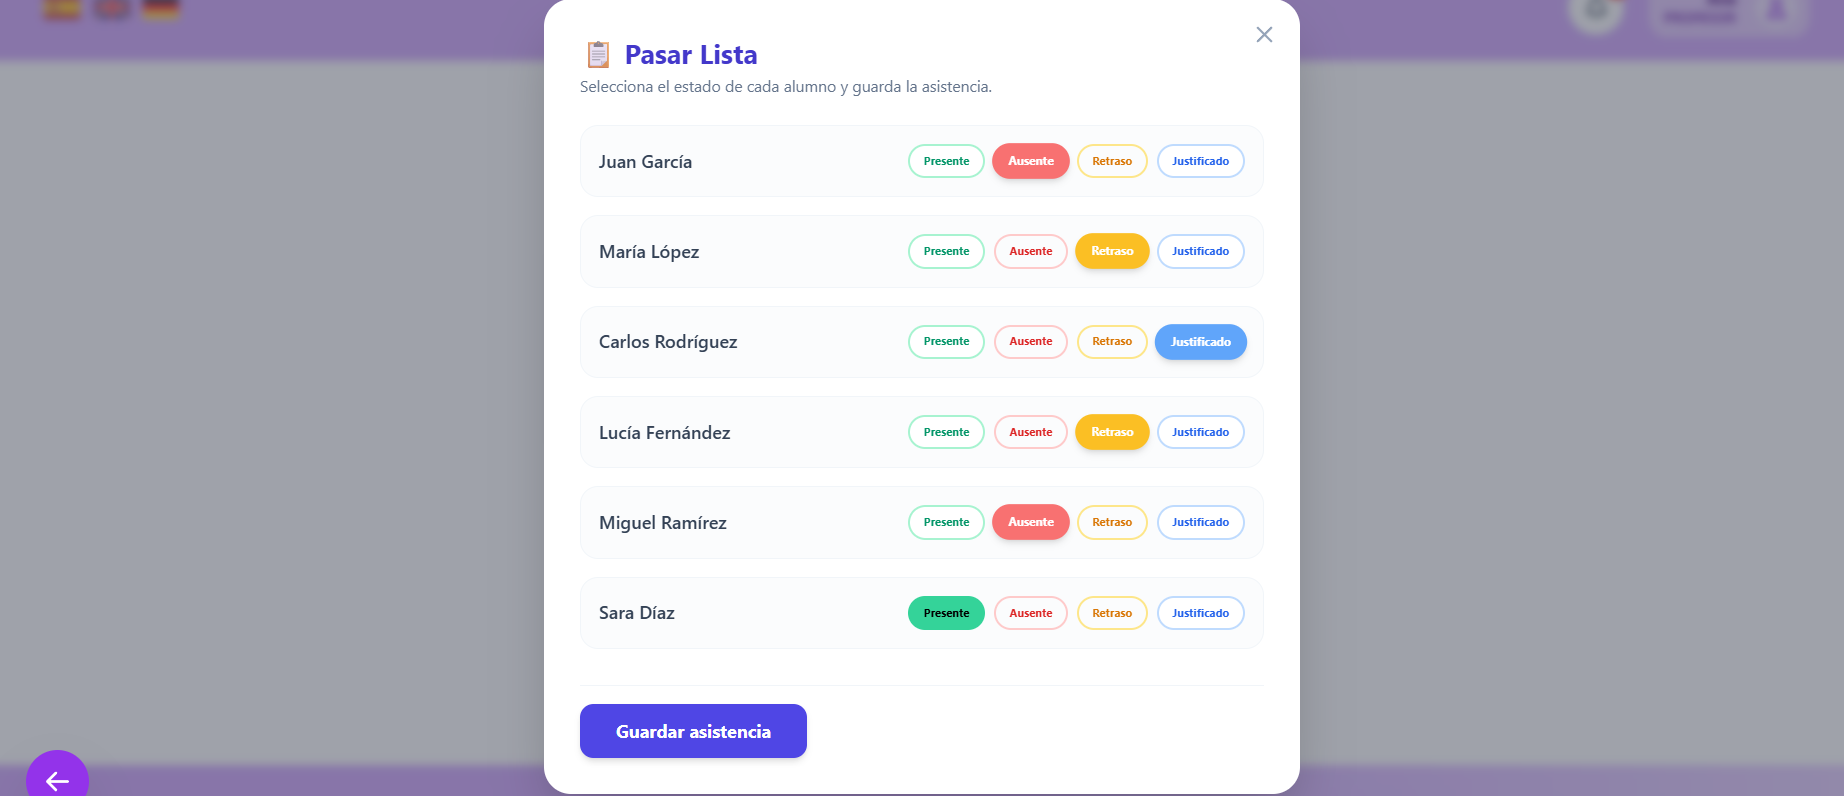
\includegraphics[keepaspectratio,alt={CAPTURA 9 --- Modal de asistencia con lista de alumnos y estados}]{../../assets/screenshots/manual-profesor/captura7-pasar_lista.png}}
\caption{CAPTURA 9 --- Modal de asistencia con lista de alumnos y
estados}
\end{figure}

\begin{figure}
\centering
\pandocbounded{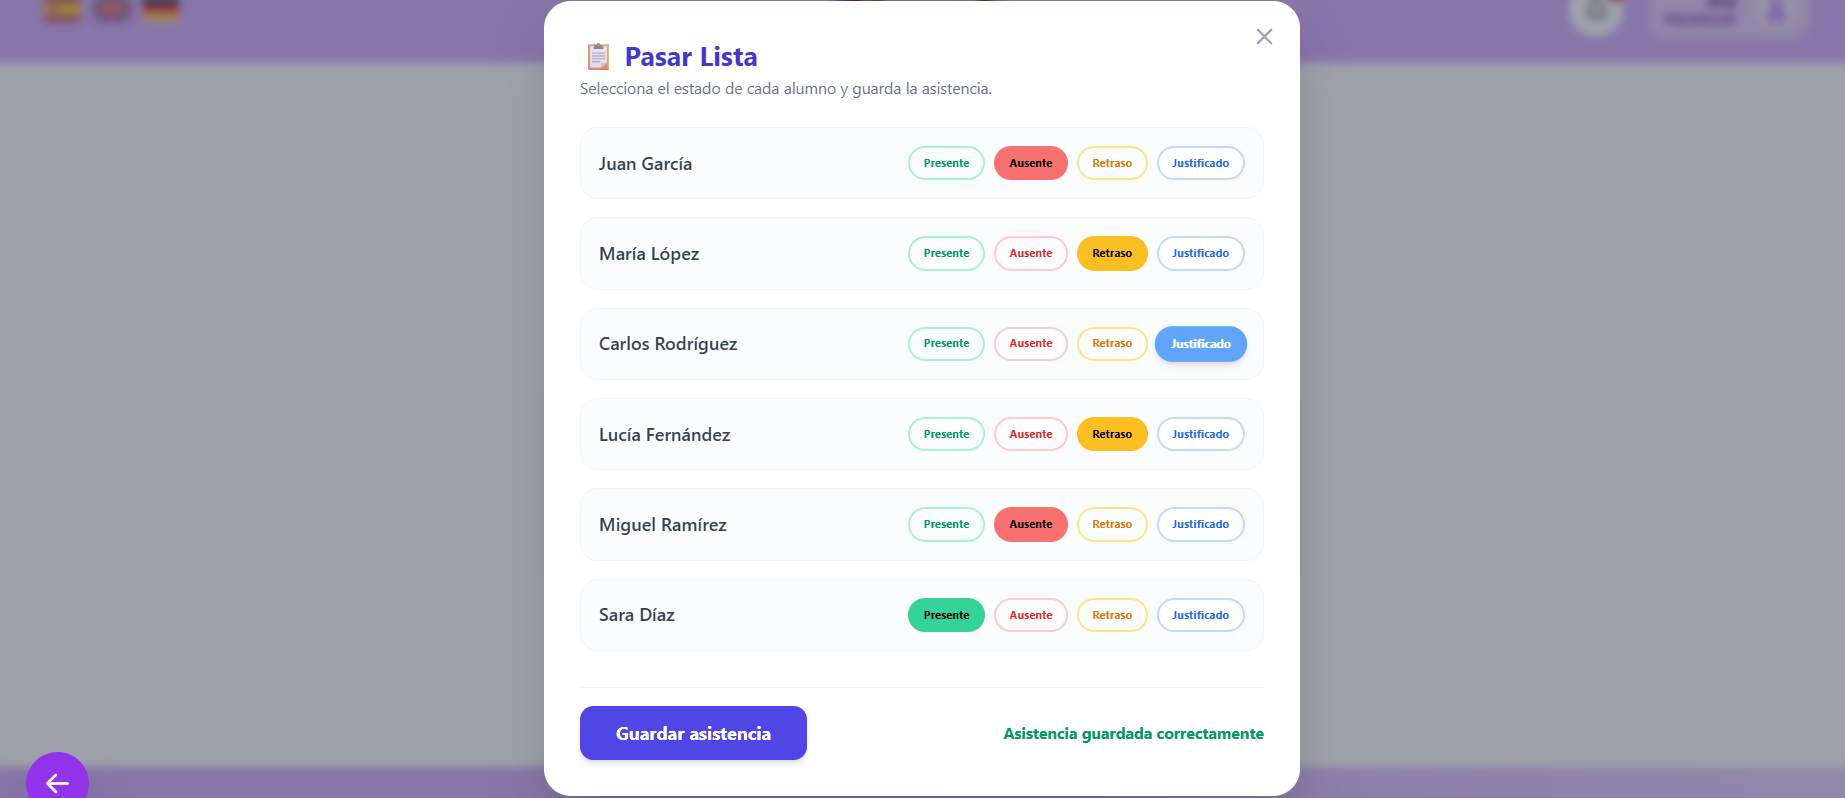
\includegraphics[keepaspectratio,alt={CAPTURA 10 --- Asistencia guardada correctamente}]{../../assets/screenshots/manual-profesor/captura10-lista_mandada.png}}
\caption{CAPTURA 10 --- Asistencia guardada correctamente}
\end{figure}

\textbf{Nota:} Debes pasar lista en la sesión correspondiente al día; si
no hay alumnos matriculados, el sistema lo indicará.

\begin{center}\rule{0.5\linewidth}{0.5pt}\end{center}

\section{8. Menú de clase}\label{menuxfa-de-clase}

Ruta: \textbf{Menú de clase} desde una tarjeta →
\texttt{/menu-clase/:idTeacherAssignment}

Pantalla intermedia con \textbf{dos opciones}:

{\def\LTcaptype{none} % do not increment counter
\begin{longtable}[]{@{}
  >{\raggedright\arraybackslash}p{(\linewidth - 4\tabcolsep) * \real{0.2963}}
  >{\raggedright\arraybackslash}p{(\linewidth - 4\tabcolsep) * \real{0.4815}}
  >{\raggedright\arraybackslash}p{(\linewidth - 4\tabcolsep) * \real{0.2222}}@{}}
\toprule\noalign{}
\begin{minipage}[b]{\linewidth}\raggedright
Opción
\end{minipage} & \begin{minipage}[b]{\linewidth}\raggedright
Descripción
\end{minipage} & \begin{minipage}[b]{\linewidth}\raggedright
Ruta
\end{minipage} \\
\midrule\noalign{}
\endhead
\bottomrule\noalign{}
\endlastfoot
\textbf{Tareas} & Crear y listar tareas de la asignación &
\texttt{/tareas/:idTeacherAssignment} \\
\textbf{Justificaciones} & Revisar justificantes de faltas &
\texttt{/ficha-profesor} (vista de justificaciones) \\
\end{longtable}
}

\begin{figure}
\centering
\pandocbounded{
\includegraphics[keepaspectratio,alt={CAPTURA 11 --- Menú de clase con tarjetas Tareas y Justificaciones}]{../../assets/screenshots/manual-profesor/captura11-menu_clase.png}}
\caption{CAPTURA 11 --- Menú de clase con tarjetas Tareas y
Justificaciones}
\end{figure}

\begin{center}\rule{0.5\linewidth}{0.5pt}\end{center}

\section{9. Gestión de tareas}\label{gestiuxf3n-de-tareas}

Ruta: \textbf{Menú de clase → Tareas}
(\texttt{/tareas/:idTeacherAssignment}).

\subsection{9.1 Listado agrupado}\label{listado-agrupado}

\begin{itemize}
\tightlist
\item
  Las tareas se agrupan por \textbf{tipo} (deberes, práctica, teoría,
  proyecto, examen) con código de color.
\item
  En la cabecera: número total de tareas y botón \textbf{+ Crear tarea}.
\item
  Cada ítem permite ver detalle y acciones según el componente de lista.
\end{itemize}

\begin{figure}
\centering
\pandocbounded{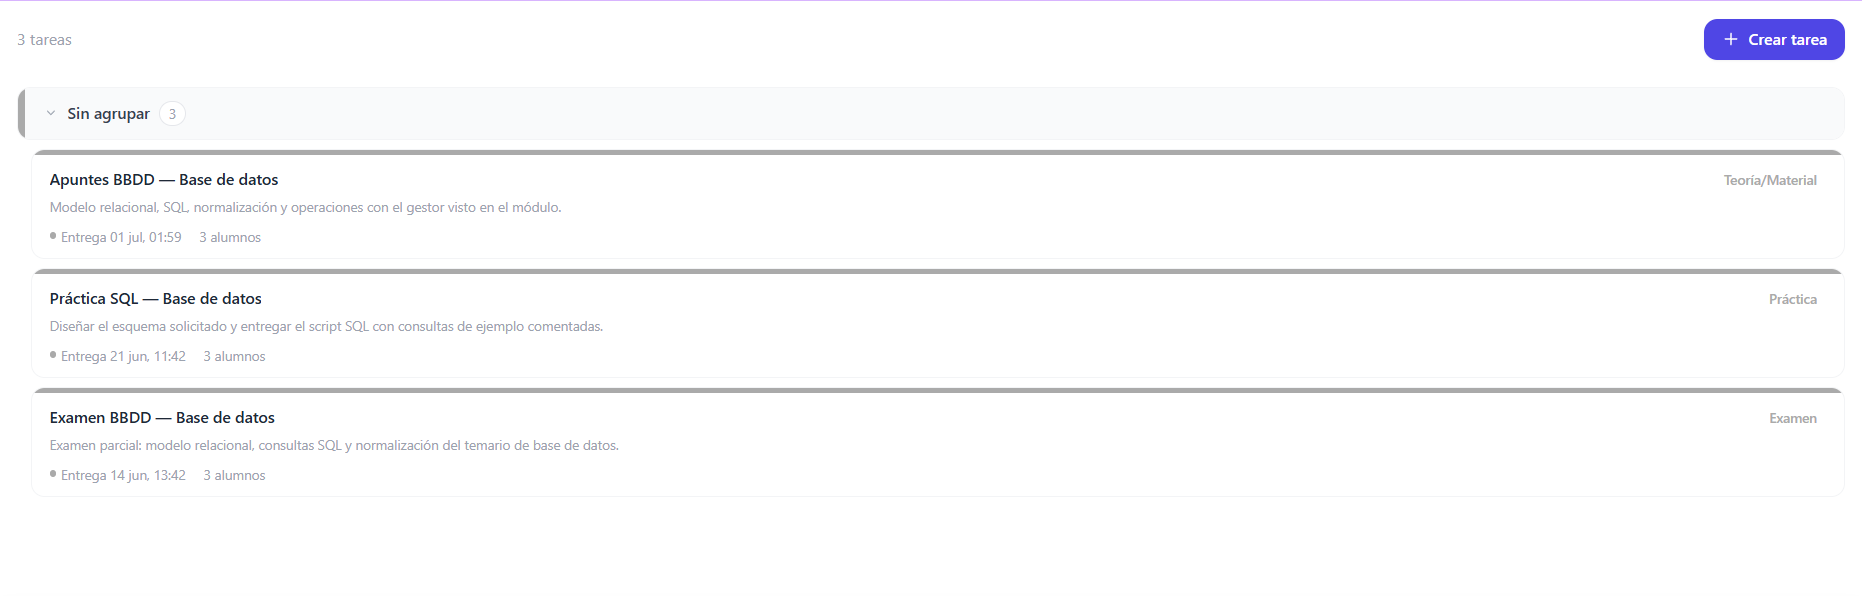
\includegraphics[keepaspectratio,alt={CAPTURA 12 --- Lista de tareas agrupadas con botón Crear tarea}]{../../assets/screenshots/manual-profesor/captura12-tareas_agrupadas.png}}
\caption{CAPTURA 12 --- Lista de tareas agrupadas con botón Crear tarea}
\end{figure}

\subsection{9.2 Crear una nueva tarea}\label{crear-una-nueva-tarea}

\begin{enumerate}
\def\labelenumi{\arabic{enumi}.}
\tightlist
\item
  Pulsa \textbf{Crear tarea} (botón indigo con icono +).
\item
  Se abre el formulario modal \textbf{Crear nueva tarea}.
\end{enumerate}

Campos del formulario:

{\def\LTcaptype{none} % do not increment counter
\begin{longtable}[]{@{}
  >{\raggedright\arraybackslash}p{(\linewidth - 4\tabcolsep) * \real{0.2121}}
  >{\raggedright\arraybackslash}p{(\linewidth - 4\tabcolsep) * \real{0.3939}}
  >{\raggedright\arraybackslash}p{(\linewidth - 4\tabcolsep) * \real{0.3939}}@{}}
\toprule\noalign{}
\begin{minipage}[b]{\linewidth}\raggedright
Campo
\end{minipage} & \begin{minipage}[b]{\linewidth}\raggedright
Obligatorio
\end{minipage} & \begin{minipage}[b]{\linewidth}\raggedright
Descripción
\end{minipage} \\
\midrule\noalign{}
\endhead
\bottomrule\noalign{}
\endlastfoot
Título & Sí & Nombre visible para el alumno \\
Descripción & No & Instrucciones de la actividad \\
Tipo & Sí & Deberes, práctica, teoría/material, proyecto, examen \\
Fecha de inicio & Sí & Cuándo se publica \\
Fecha límite & Sí & Deadline de entrega \\
Fichero adjunto & No & Material de apoyo (PDF, DOCX, ZIP, PNG, JPG; máx.
10 MB) \\
Permite entrega tardía & Según diseño & Si está activo, los alumnos
pueden entregar fuera de plazo (marcado LATE) \\
\end{longtable}
}

\begin{enumerate}
\def\labelenumi{\arabic{enumi}.}
\setcounter{enumi}{2}
\tightlist
\item
  Opcional: arrastra un archivo o selecciónalo.
\item
  Pulsa \textbf{Crear tarea}.
\item
  Tras el éxito, la tarea aparecerá en el listado y en el
  \textbf{temario} del alumno.
\end{enumerate}

\begin{figure}
\centering
\pandocbounded{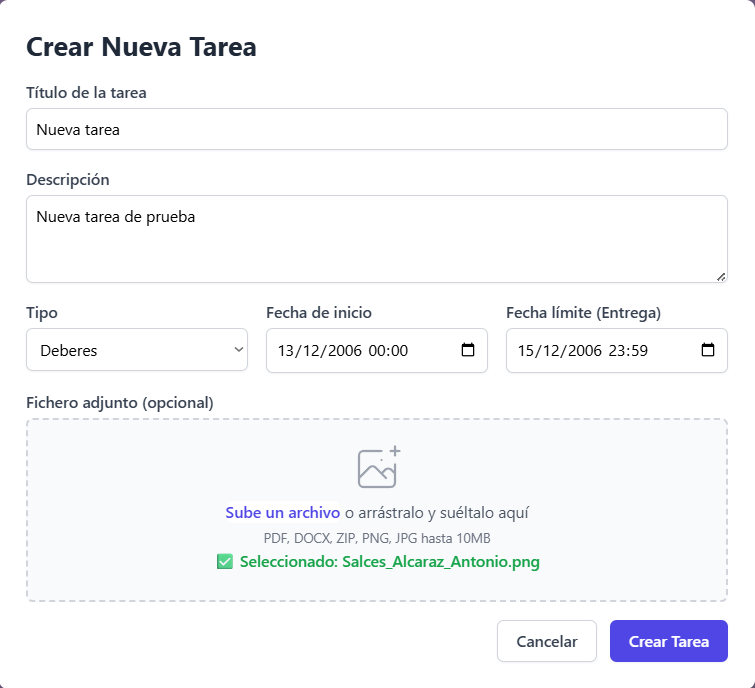
\includegraphics[keepaspectratio,alt={CAPTURA 13 --- Formulario Crear nueva tarea y confirmación}]{../../assets/screenshots/manual-profesor/captura13-guardar_tarea.png}}
\caption{CAPTURA 13 --- Formulario Crear nueva tarea y confirmación}
\end{figure}

\subsection{9.3 Errores al crear tarea}\label{errores-al-crear-tarea}

\begin{itemize}
\tightlist
\item
  Archivo mayor de 10 MB → error de tamaño.
\item
  Error de servidor → revisa conexión y reintenta.
\end{itemize}

\begin{center}\rule{0.5\linewidth}{0.5pt}\end{center}

\section{10. Entregas de los alumnos}\label{entregas-de-los-alumnos}

Ruta: \textbf{Temario → Ver entregas} o desde detalle de tarea →
\texttt{/tarea/:taskId/entregas}

\subsection{10.1 Pantalla de entregas}\label{pantalla-de-entregas}

Información mostrada:

\begin{itemize}
\tightlist
\item
  Título de la tarea y \textbf{fecha límite}
\item
  Tabla o listado con columnas: \textbf{Alumno}, \textbf{Estado},
  \textbf{Fecha entrega}, \textbf{Nota}, \textbf{Acciones}
\end{itemize}

Estados habituales:

{\def\LTcaptype{none} % do not increment counter
\begin{longtable}[]{@{}ll@{}}
\toprule\noalign{}
Estado & Significado \\
\midrule\noalign{}
\endhead
\bottomrule\noalign{}
\endlastfoot
Pendiente & Sin entrega \\
Entregada & Entrega a tiempo \\
Retraso / Entregada tarde & Fuera de plazo permitido \\
Calificada & Ya tiene nota \\
No entregado & Plazo cerrado sin entrega \\
\end{longtable}
}

\begin{figure}
\centering
\pandocbounded{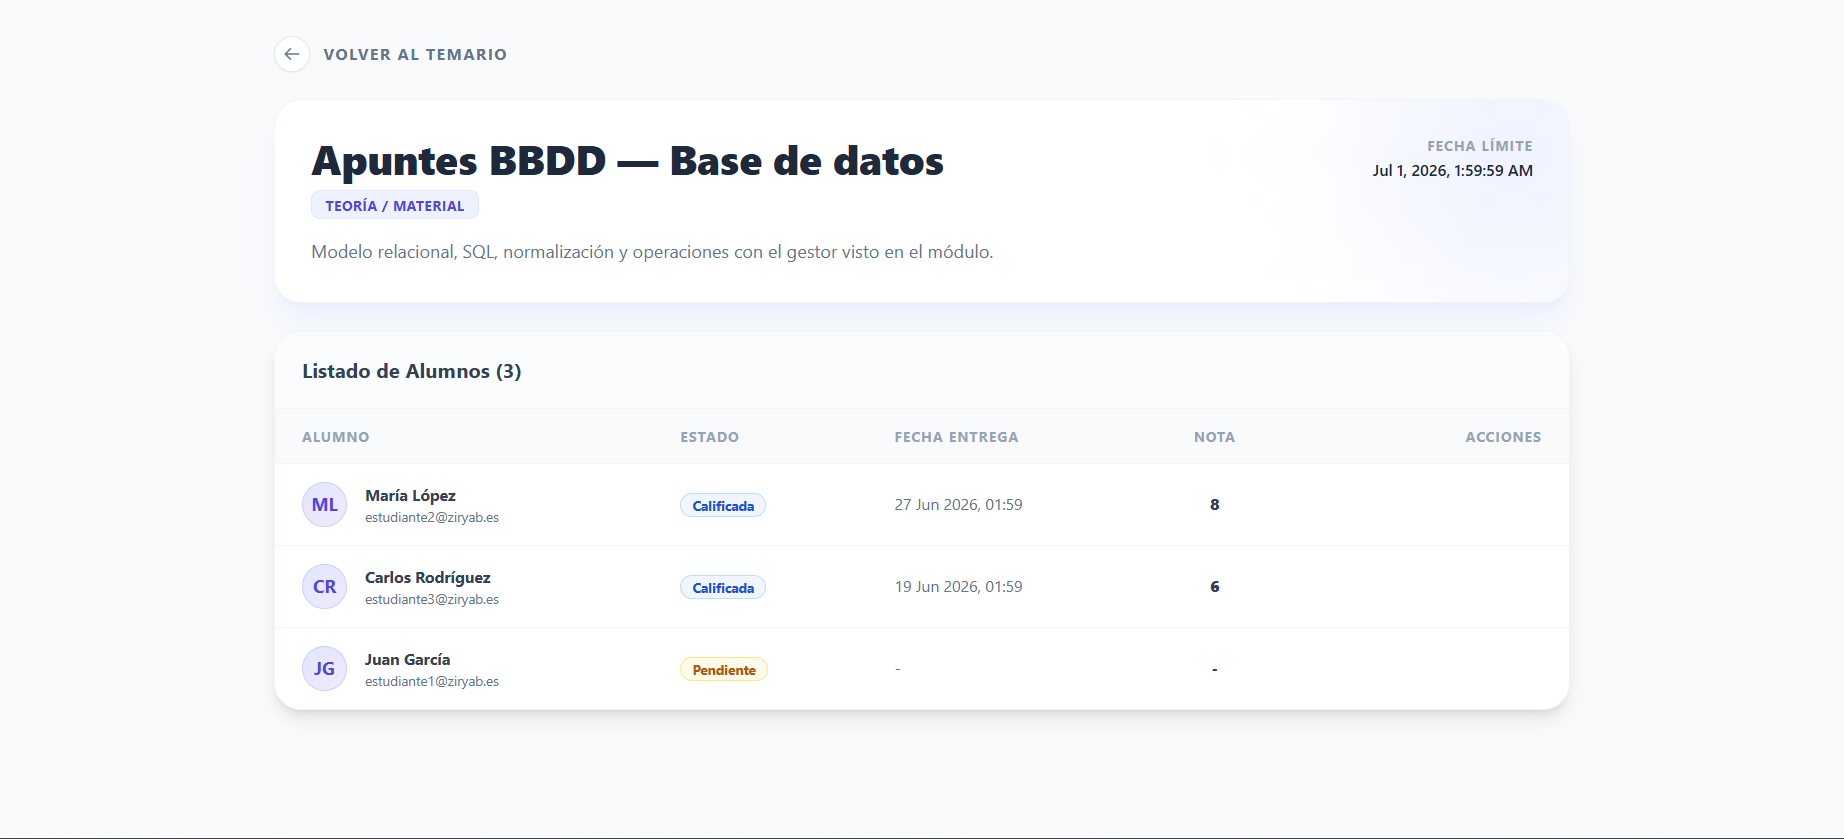
\includegraphics[keepaspectratio,alt={CAPTURA 15 --- Listado de entregas con varios estados}]{../../assets/screenshots/manual-profesor/captura15-listado_tareas.png}}
\caption{CAPTURA 15 --- Listado de entregas con varios estados}
\end{figure}

\subsection{10.2 Acciones por entrega}\label{acciones-por-entrega}

\begin{itemize}
\tightlist
\item
  \textbf{Abrir archivo/enlace} de la resolución del alumno (si
  entregó).
\item
  \textbf{Calificar} o \textbf{Editar nota} --- Abre la pantalla de
  corrección.
\end{itemize}

\begin{center}\rule{0.5\linewidth}{0.5pt}\end{center}

\section{11. Calificar una entrega}\label{calificar-una-entrega}

Ruta: \texttt{/calificar-tarea/:id} (ID de la entrega del alumno)

\subsection{11.1 Datos de la entrega}\label{datos-de-la-entrega}

La pantalla muestra:

\begin{itemize}
\tightlist
\item
  Nombre del \textbf{alumno}
\item
  \textbf{Tarea} evaluada
\item
  \textbf{Momento de entrega} (fecha/hora)
\item
  \textbf{Archivo entregado} --- enlace Ver / Descargar
\end{itemize}

\subsection{11.2 Formulario de
corrección}\label{formulario-de-correcciuxf3n}

{\def\LTcaptype{none} % do not increment counter
\begin{longtable}[]{@{}ll@{}}
\toprule\noalign{}
Campo & Reglas \\
\midrule\noalign{}
\endhead
\bottomrule\noalign{}
\endlastfoot
Calificación (0--10) & Obligatoria; valor entre 0 y 10 \\
Comentarios y feedback & Opcional; visible para el alumno \\
\end{longtable}
}

\begin{enumerate}
\def\labelenumi{\arabic{enumi}.}
\tightlist
\item
  Introduce la \textbf{nota}.
\item
  Opcional: escribe observaciones en \textbf{Feedback}.
\item
  Pulsa \textbf{Guardar calificación}.
\end{enumerate}

\begin{figure}
\centering
\pandocbounded{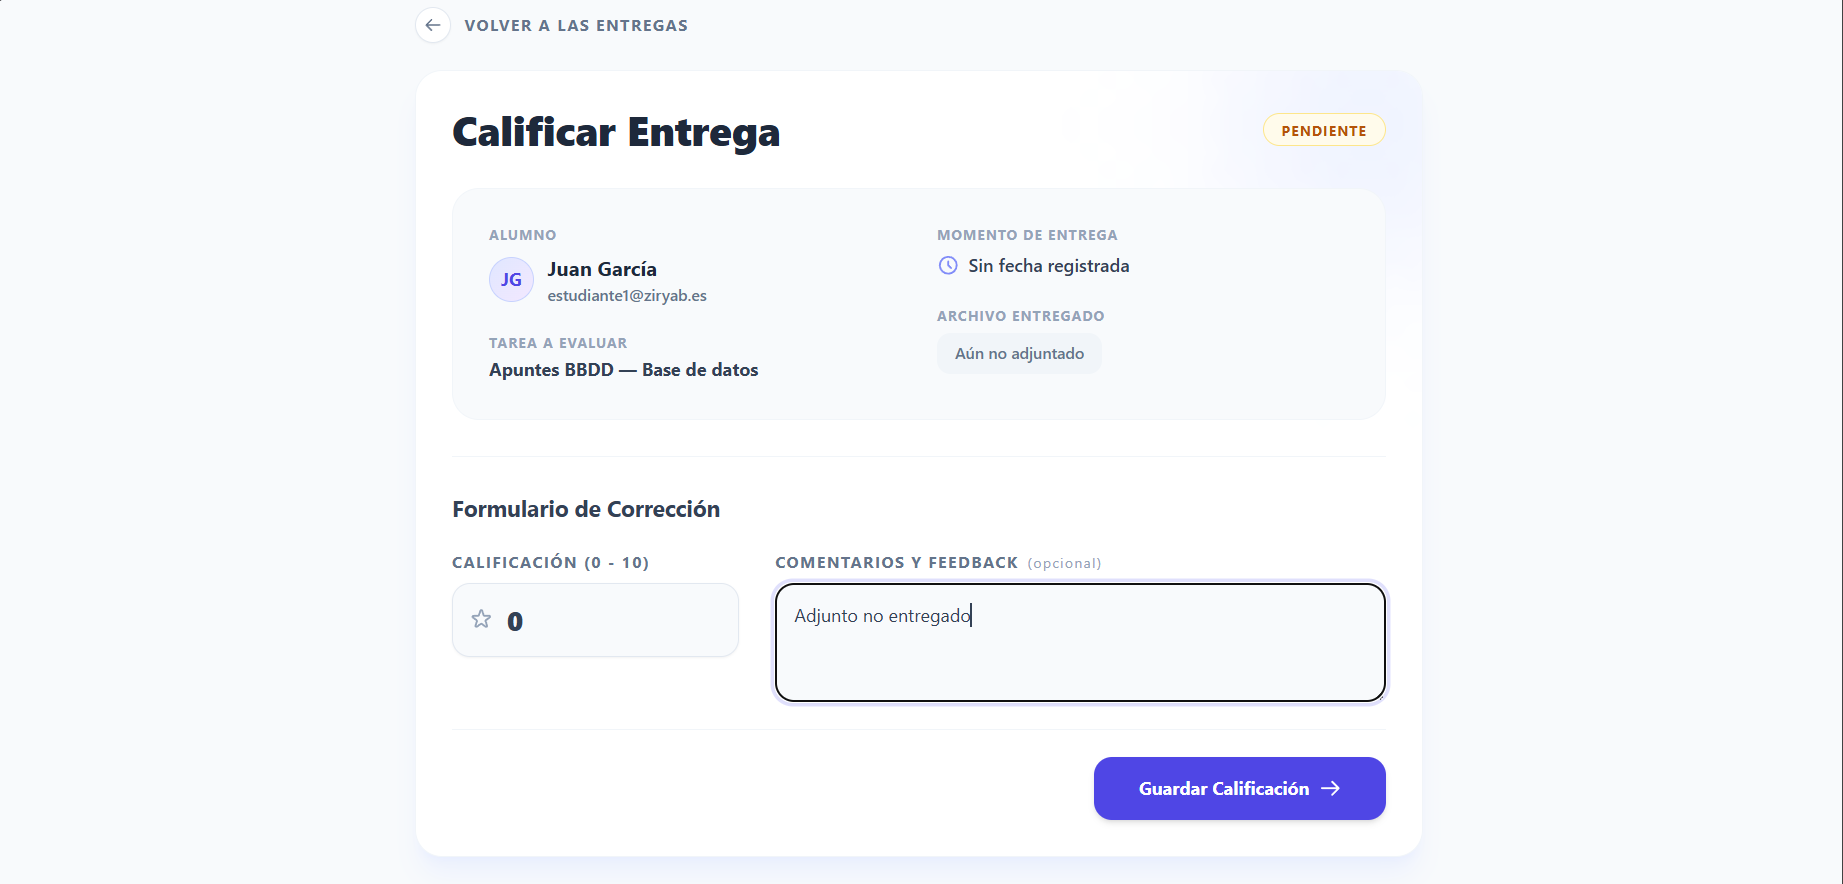
\includegraphics[keepaspectratio,alt={CAPTURA 16 --- Pantalla Calificar entrega}]{../../assets/screenshots/manual-profesor/captura16-calificar_entrega.png}}
\caption{CAPTURA 16 --- Pantalla Calificar entrega}
\end{figure}

El alumno verá la nota en su detalle de tarea y en el temario (estado
CALIFICADA).

\begin{center}\rule{0.5\linewidth}{0.5pt}\end{center}

\section{12. Justificaciones de faltas}\label{justificaciones-de-faltas}

Ruta: \textbf{Menú de clase → Justificaciones} o ficha de profesor
(\texttt{/ficha-profesor}).

\subsection{12.1 Justificaciones
pendientes}\label{justificaciones-pendientes}

\begin{itemize}
\tightlist
\item
  Listado de alumnos que han subido un \textbf{justificante} en estado
  pendiente.
\item
  Por cada fila: nombre del alumno, fecha/hora de la sesión, asignatura.
\item
  Acciones:

  \begin{itemize}
  \tightlist
  \item
    \textbf{Ver archivo} --- Abre el documento subido (PDF/imagen)
  \item
    \textbf{Aceptar} --- La falta pasa a justificada
  \item
    \textbf{Rechazar} --- El justificante se rechaza; el alumno puede
    volver a enviar otro
  \end{itemize}
\end{itemize}

\begin{figure}
\centering
\pandocbounded{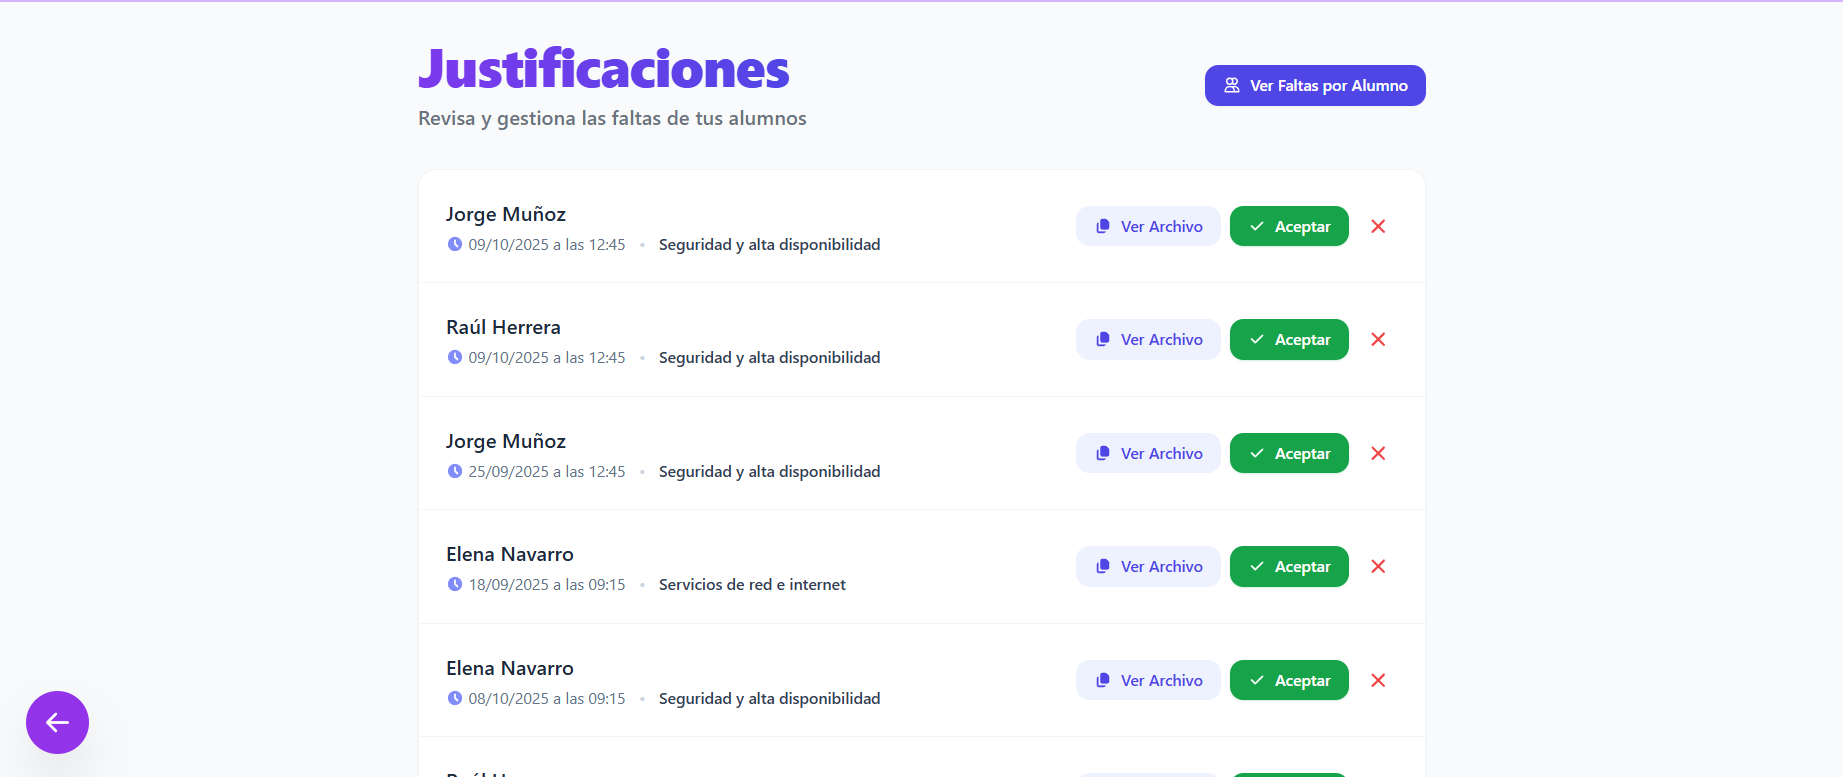
\includegraphics[keepaspectratio,alt={CAPTURA 19 --- Lista de justificaciones pendientes}]{../../assets/screenshots/manual-profesor/captura19-justificaciones_pendientes.png}}
\caption{CAPTURA 19 --- Lista de justificaciones pendientes}
\end{figure}

\subsection{12.2 Sin pendientes}\label{sin-pendientes}

Mensaje: \emph{«Todo al día»} / \emph{«No hay nuevas justificaciones
pendientes de revisar»}.

\subsection{12.3 Ver faltas por alumno}\label{ver-faltas-por-alumno}

\begin{itemize}
\tightlist
\item
  Botón \textbf{Ver faltas por alumno} (parte superior).
\item
  Abre un modal para consultar el historial de ausencias de un
  estudiante concreto.
\end{itemize}

\begin{figure}
\centering
\pandocbounded{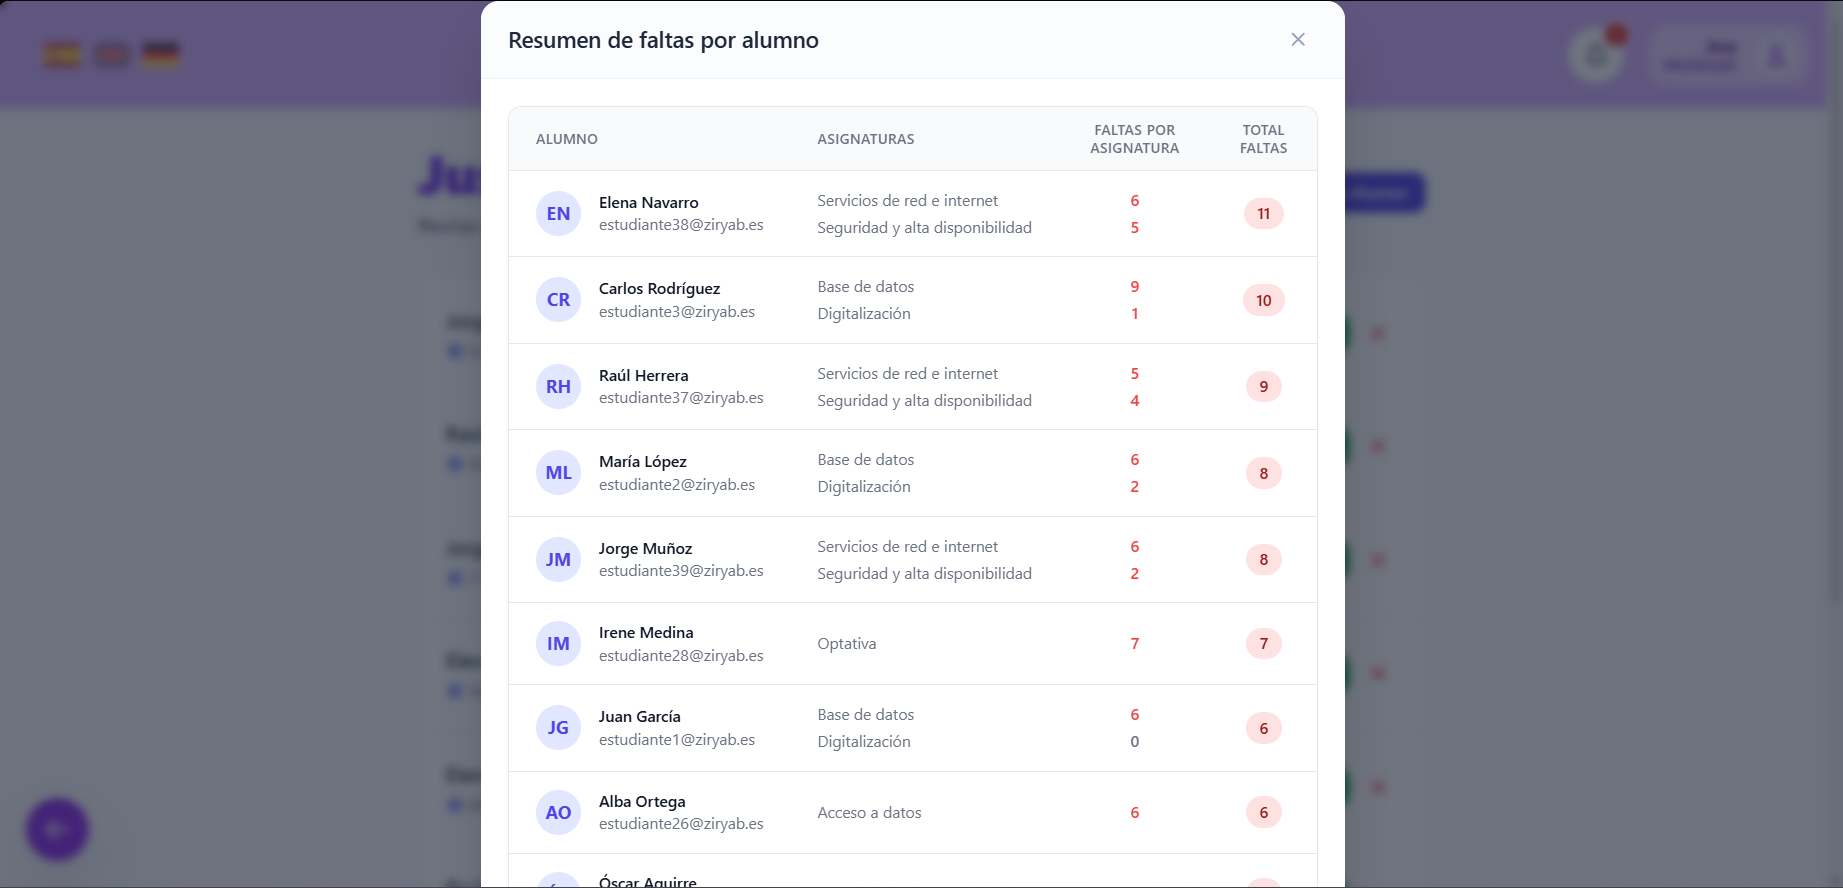
\includegraphics[keepaspectratio,alt={CAPTURA 21 --- Modal de faltas por alumno}]{../../assets/screenshots/manual-profesor/captura21-faltas_por_alumno.png}}
\caption{CAPTURA 21 --- Modal de faltas por alumno}
\end{figure}

\begin{center}\rule{0.5\linewidth}{0.5pt}\end{center}

\section{13. Gestión académica (área
común)}\label{gestiuxf3n-acaduxe9mica-uxe1rea-comuxfan}

Ruta: \textbf{Mi Espacio → Gestión} (\texttt{/gestion}).

Las mismas tarjetas que el alumno, con rutas adaptadas al rol:

{\def\LTcaptype{none} % do not increment counter
\begin{longtable}[]{@{}
  >{\raggedright\arraybackslash}p{(\linewidth - 2\tabcolsep) * \real{0.3333}}
  >{\raggedright\arraybackslash}p{(\linewidth - 2\tabcolsep) * \real{0.6667}}@{}}
\toprule\noalign{}
\begin{minipage}[b]{\linewidth}\raggedright
Tarjeta
\end{minipage} & \begin{minipage}[b]{\linewidth}\raggedright
Destino profesor
\end{minipage} \\
\midrule\noalign{}
\endhead
\bottomrule\noalign{}
\endlastfoot
Ficha Usuario & \texttt{/ficha-usuario} (datos personales; según
configuración) \\
Horario & \texttt{/horario-profesor} \\
Calendario & \texttt{/calendario} \\
Tablón & \texttt{/issues} \\
Evaluaciones & \texttt{/evaluaciones} (solo si eres \textbf{tutor} de un
grupo) \\
\end{longtable}
}

\begin{figure}
\centering
\pandocbounded{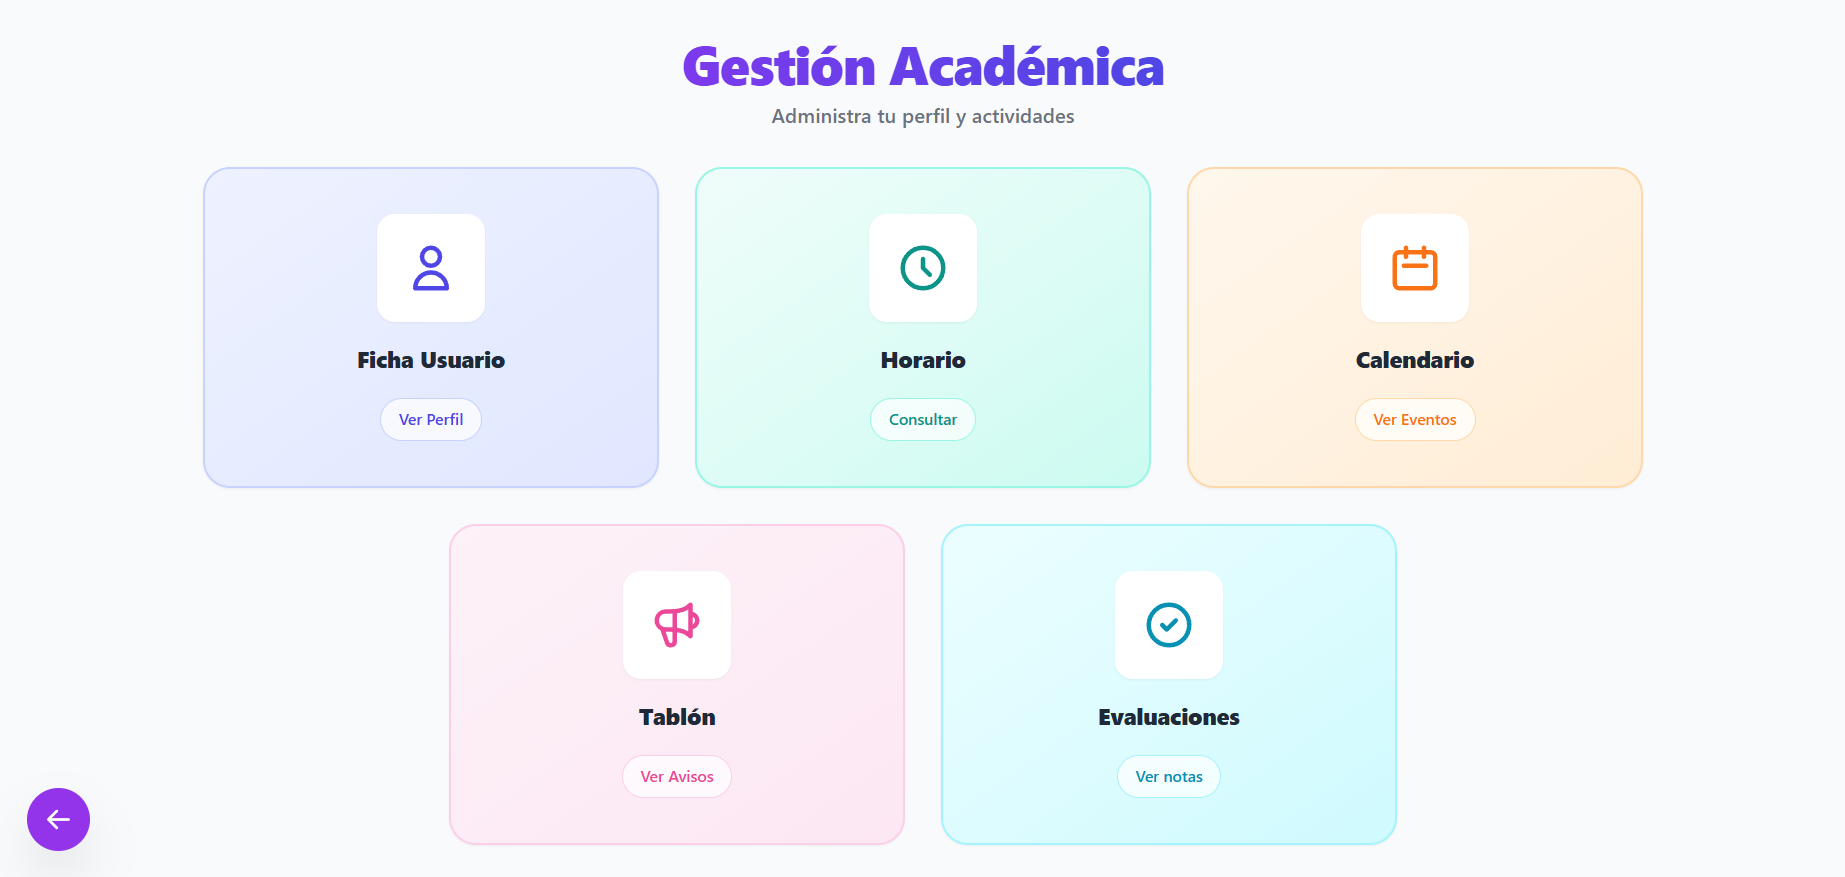
\includegraphics[keepaspectratio,alt={CAPTURA 22 --- Gestión académica vista como profesor}]{../../assets/screenshots/manual-profesor/captura22-gestion.png}}
\caption{CAPTURA 22 --- Gestión académica vista como profesor}
\end{figure}

\begin{center}\rule{0.5\linewidth}{0.5pt}\end{center}

\section{14. Horario del profesor}\label{horario-del-profesor}

Ruta: \textbf{Gestión → Horario} (\texttt{/horario-profesor}).

\begin{itemize}
\tightlist
\item
  Cuadrícula semanal con tus \textbf{franjas de clase} asignadas.
\item
  Cada celda indica hora y asignatura/grupo.
\end{itemize}

\begin{figure}
\centering
\pandocbounded{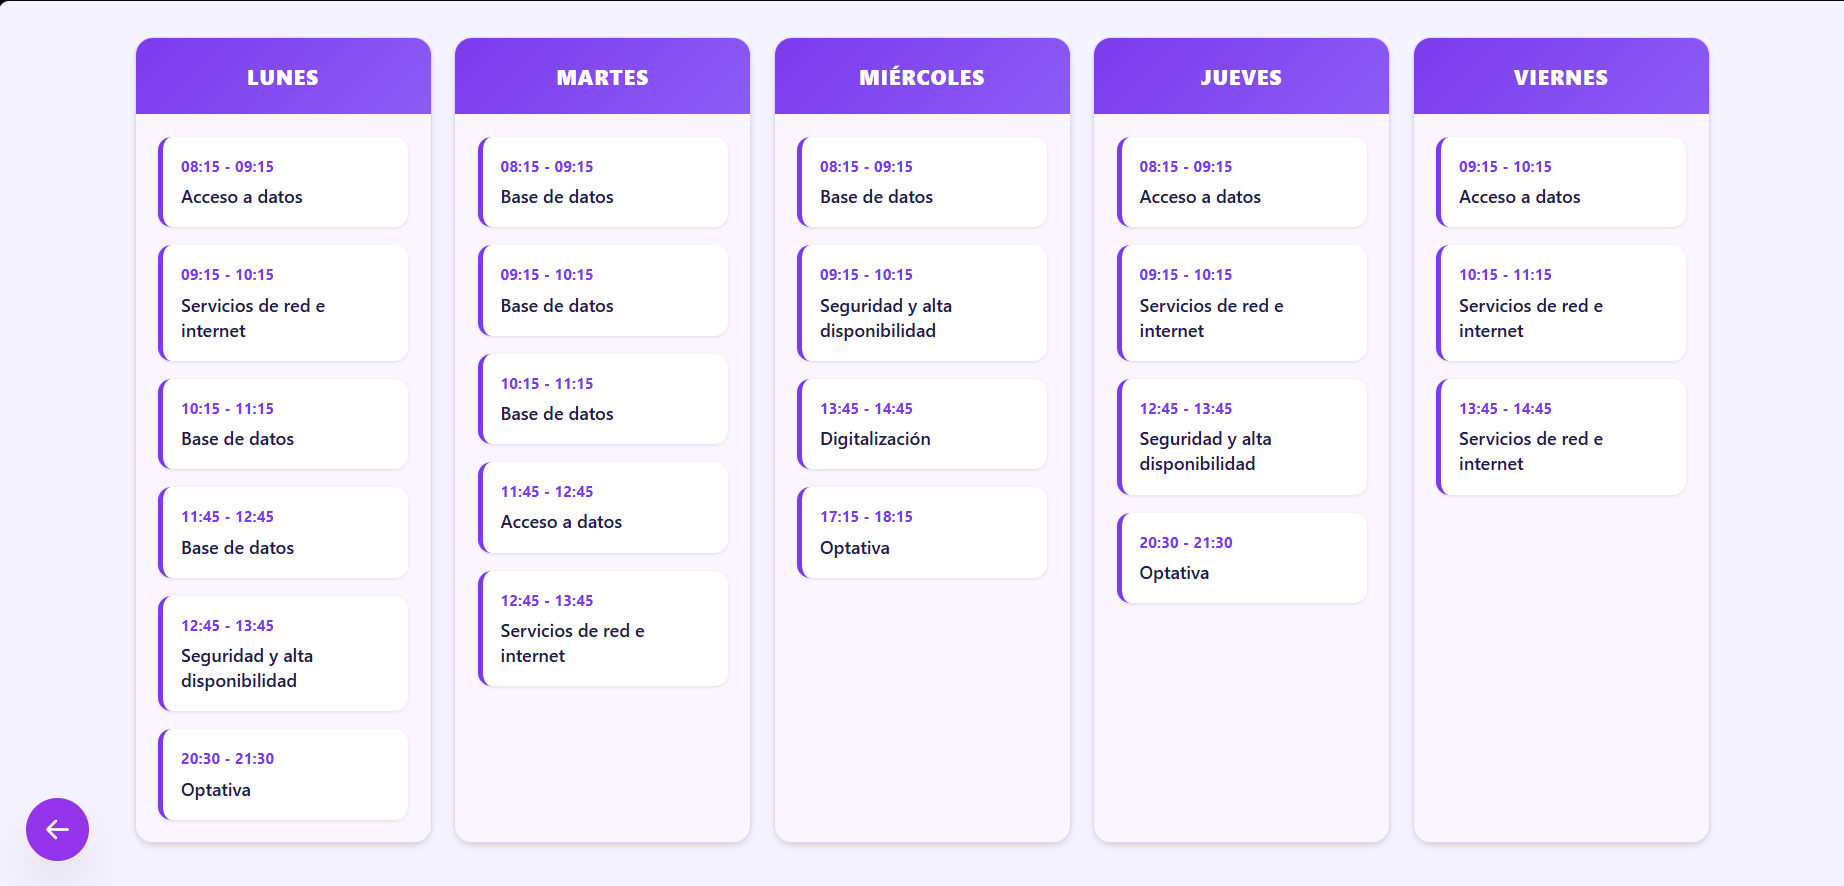
\includegraphics[keepaspectratio,alt={CAPTURA 23 --- Horario semanal del profesor}]{../../assets/screenshots/manual-profesor/captura23-horario.png}}
\caption{CAPTURA 23 --- Horario semanal del profesor}
\end{figure}

\begin{center}\rule{0.5\linewidth}{0.5pt}\end{center}

\section{15. Calendario y tablón}\label{calendario-y-tabluxf3n}

\begin{itemize}
\tightlist
\item
  \textbf{Calendario:} iframe con el calendario institucional
  (\texttt{/calendario}).
\item
  \textbf{Tablón:} anuncios publicados para toda la comunidad
  (\texttt{/issues}).
\end{itemize}

\begin{figure}
\centering
\pandocbounded{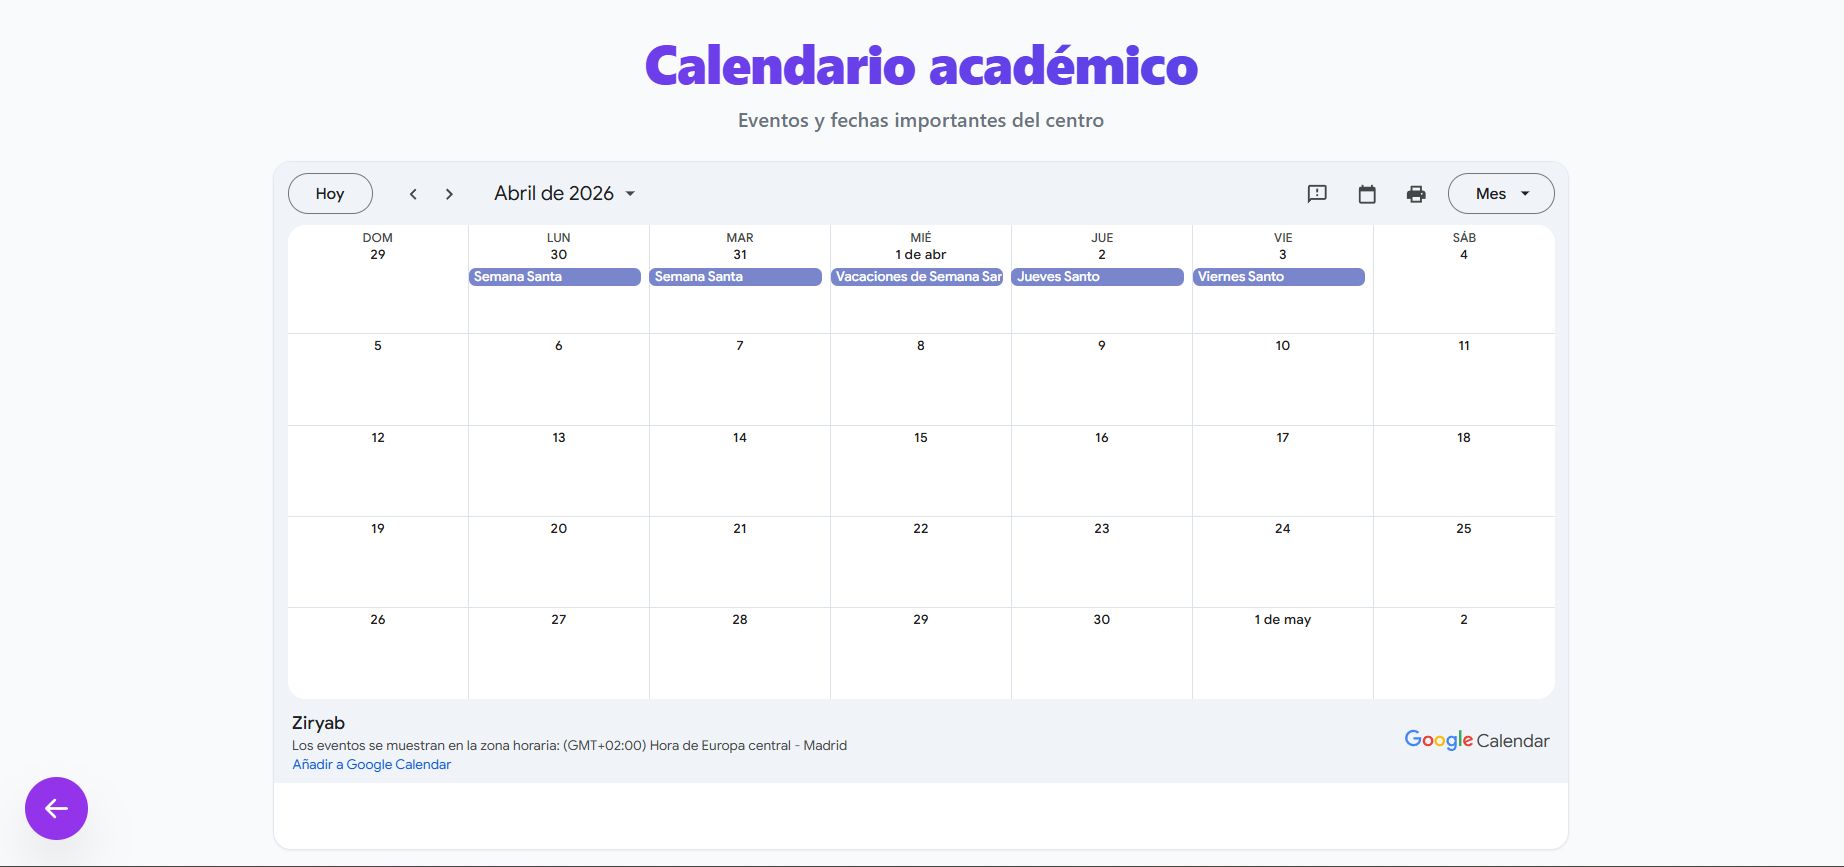
\includegraphics[keepaspectratio,alt={CAPTURA 24 --- Calendario embebido}]{../../assets/screenshots/manual-profesor/captura24-calendario.png}}
\caption{CAPTURA 24 --- Calendario embebido}
\end{figure}

\begin{figure}
\centering
\pandocbounded{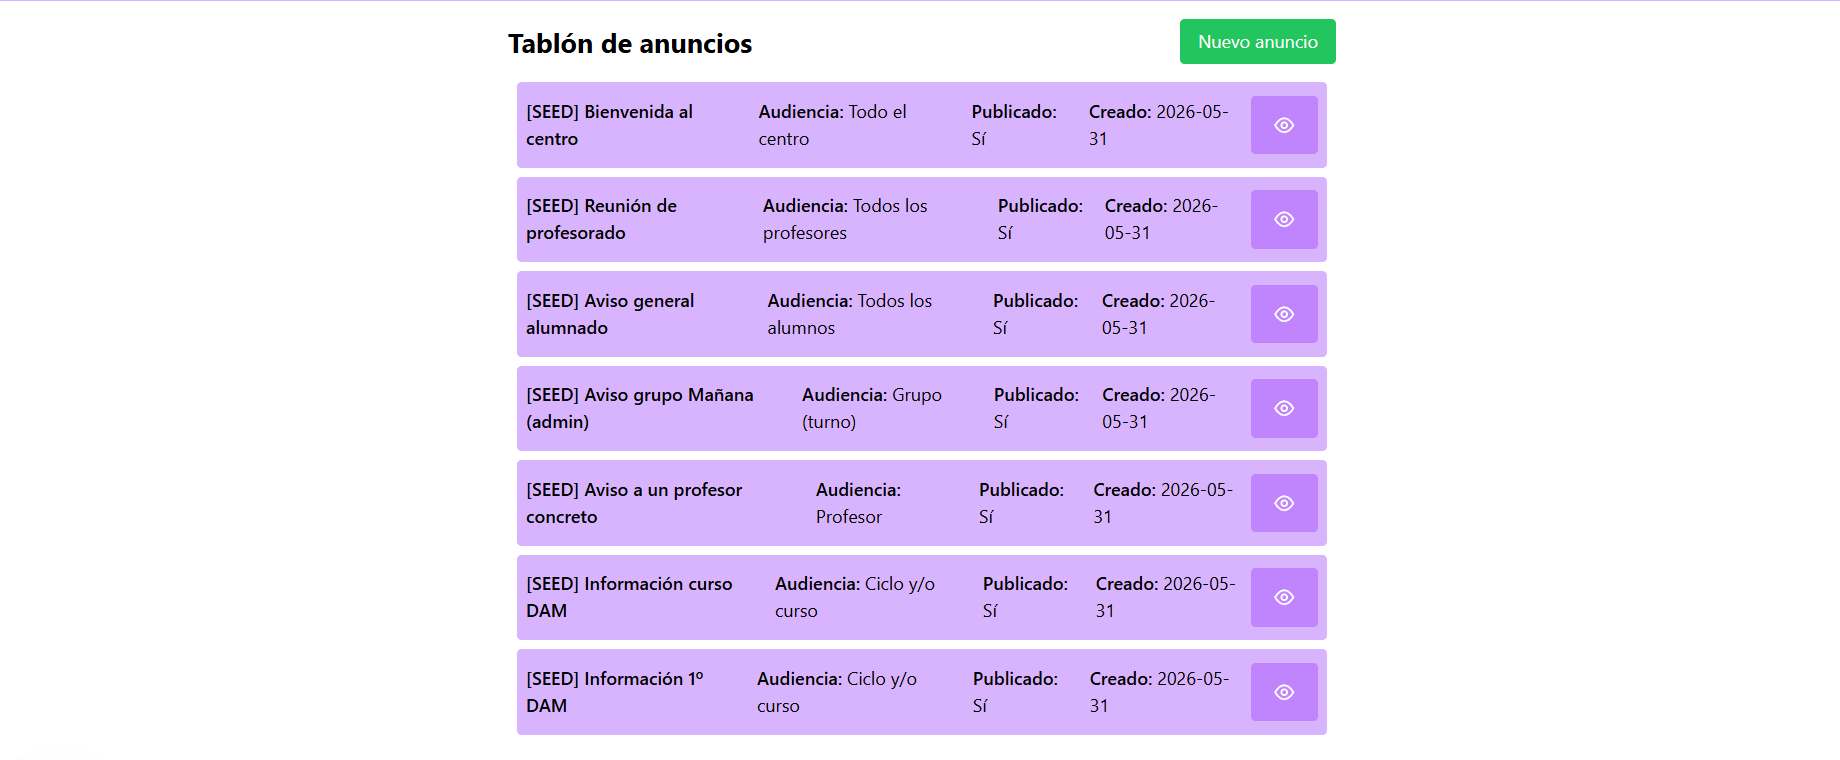
\includegraphics[keepaspectratio,alt={CAPTURA 25 --- Tablón de anuncios}]{../../assets/screenshots/manual-profesor/captura25-tablon.png}}
\caption{CAPTURA 25 --- Tablón de anuncios}
\end{figure}

\subsection{15.1 Crear un anuncio en el
tablón}\label{crear-un-anuncio-en-el-tabluxf3n}

\begin{enumerate}
\def\labelenumi{\arabic{enumi}.}
\tightlist
\item
  Accede al \textbf{Tablón} desde Gestión.
\item
  Pulsa la opción para \textbf{crear un nuevo anuncio} (si tu rol lo
  permite).
\item
  Rellena título y contenido del aviso.
\item
  Publica el anuncio; quedará visible para la comunidad educativa.
\end{enumerate}

\begin{figure}
\centering
\pandocbounded{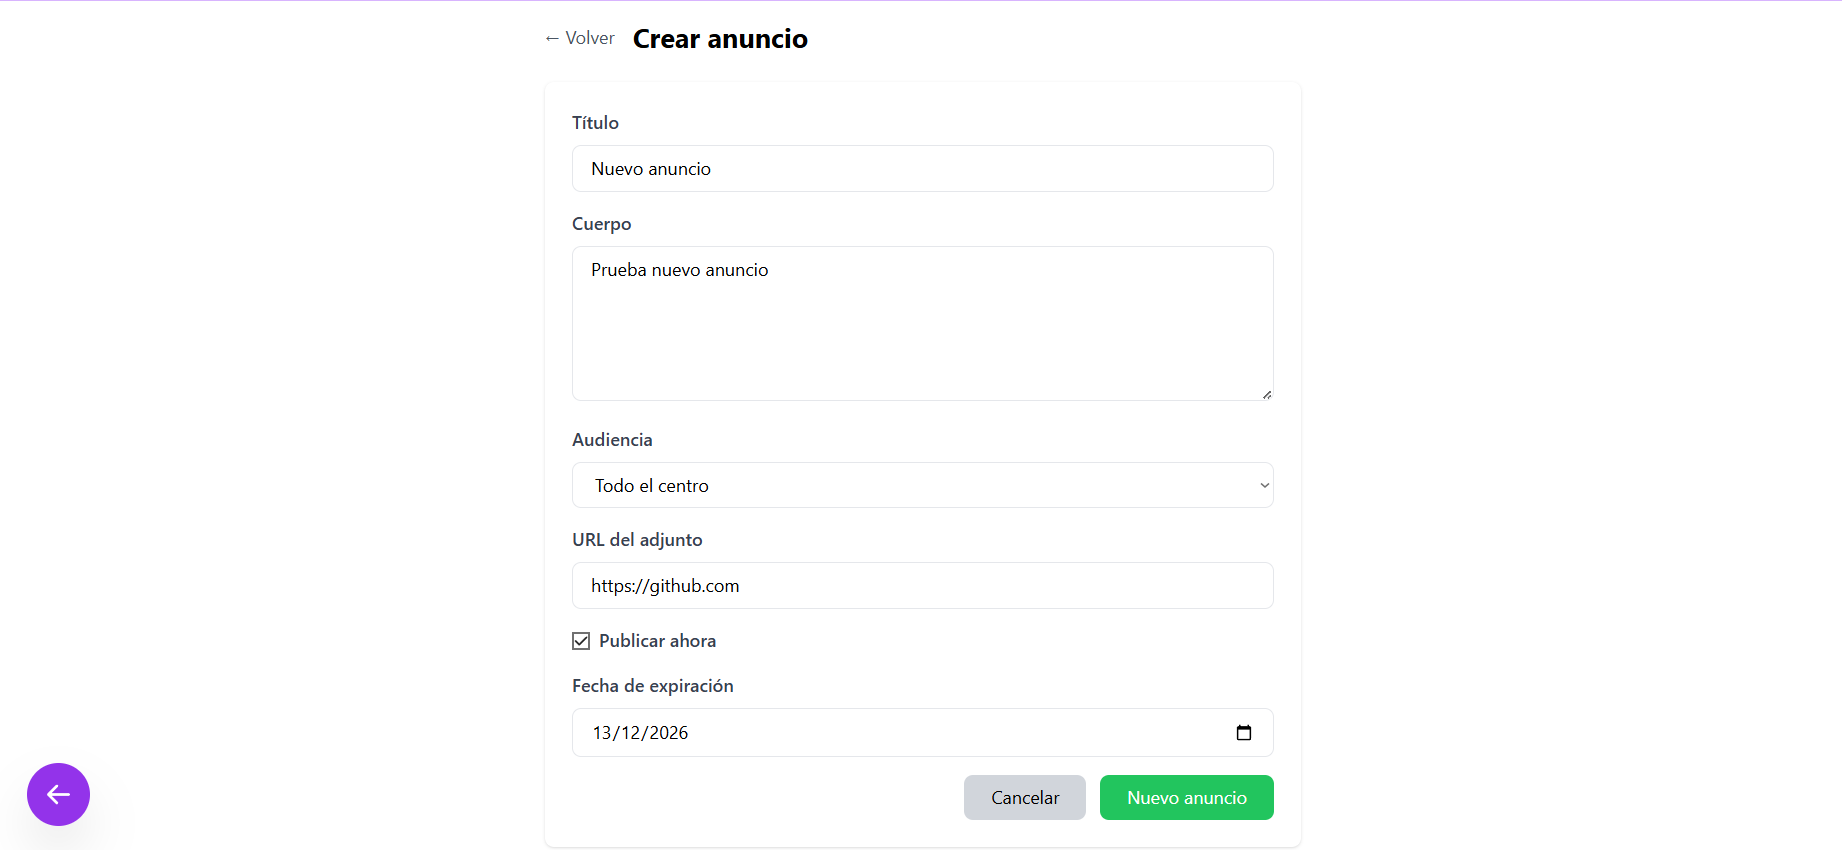
\includegraphics[keepaspectratio,alt={CAPTURA 25.2 --- Formulario crear anuncio}]{../../assets/screenshots/manual-profesor/captura25_2-crear_anuncio.png}}
\caption{CAPTURA 25.2 --- Formulario crear anuncio}
\end{figure}

\begin{center}\rule{0.5\linewidth}{0.5pt}\end{center}

\section{16. Evaluaciones (rol de
tutor)}\label{evaluaciones-rol-de-tutor}

Ruta: \textbf{Gestión → Evaluaciones} (\texttt{/evaluaciones}).

\textbf{Solo disponible si el sistema te tiene registrado como tutor de
un grupo.}

\subsection{16.1 Pantalla principal}\label{pantalla-principal}

\begin{itemize}
\tightlist
\item
  Selector de \textbf{grupo tutorizado} (si hubiera más de uno).
\item
  Selector de \textbf{periodo de evaluación} (inicial, trimestres,
  final).
\item
  Tabla: filas = alumnos del grupo; columnas = asignaturas; celdas =
  notas (1--10).
\item
  Fila o indicador de \textbf{media} por alumno/asignatura.
\end{itemize}

\begin{quote}
\textbf{📷 CAPTURA 26 --- Pantalla Evaluaciones con tabla de notas del
grupo}
\end{quote}

\subsection{16.2 Introducir y guardar
notas}\label{introducir-y-guardar-notas}

\begin{enumerate}
\def\labelenumi{\arabic{enumi}.}
\tightlist
\item
  Selecciona el \textbf{periodo} correcto.
\item
  Rellena todas las celdas obligatorias con notas entre \textbf{1 y 10}.
\item
  Pulsa \textbf{Guardar evaluaciones}.
\item
  Espera el mensaje de éxito.
\end{enumerate}

\textbf{Importante:} El sistema puede exigir que \textbf{todas} las
asignaturas de \textbf{todos} los alumnos tengan nota antes de guardar.

\begin{quote}
\textbf{📷 CAPTURA 27 --- Mensaje de notas guardadas correctamente}
\end{quote}

\subsection{16.3 Sin grupo tutorizado}\label{sin-grupo-tutorizado}

Si no eres tutor, verás: \emph{«No se ha encontrado ningún grupo del que
seas tutor»}.

\begin{center}\rule{0.5\linewidth}{0.5pt}\end{center}

\section{17. Flujos de trabajo
recomendados}\label{flujos-de-trabajo-recomendados}

\subsection{17.1 Publicar una tarea y
calificarla}\label{publicar-una-tarea-y-calificarla}

\begin{Shaded}
\begin{Highlighting}[]
\NormalTok{Mis clases → Gestionar temario → (o Menú de clase → Tareas) → Crear tarea}
\NormalTok{→ Alumnos entregan → Ver entregas → Calificar → Alumno ve la nota}
\end{Highlighting}
\end{Shaded}

\subsection{17.2 Sesión de clase con
asistencia}\label{sesiuxf3n-de-clase-con-asistencia}

\begin{Shaded}
\begin{Highlighting}[]
\NormalTok{Mis clases → Gestionar temario → Pasar lista → Guardar asistencia}
\end{Highlighting}
\end{Shaded}

\subsection{17.3 Revisar una ausencia
justificada}\label{revisar-una-ausencia-justificada}

\begin{Shaded}
\begin{Highlighting}[]
\NormalTok{Menú de clase → Justificaciones → Ver archivo → Aceptar o Rechazar}
\end{Highlighting}
\end{Shaded}

\begin{center}\rule{0.5\linewidth}{0.5pt}\end{center}

\section{18. Preguntas frecuentes
(FAQ)}\label{preguntas-frecuentes-faq-1}

\textbf{¿Por qué no veo Evaluaciones en Gestión?}\\
Esa pantalla es solo para profesores \textbf{tutores}. La asignación la
realiza administración.

\textbf{Un alumno dice que no puede entregar}\\
Comprueba la \textbf{fecha límite} y si la tarea permite \textbf{entrega
tardía}. Revisa en el detalle de la tarea.

\textbf{¿Puedo cambiar una nota ya guardada?}\\
Sí; vuelve a \textbf{Ver entregas → Editar nota} en la entrega del
alumno.

\textbf{El archivo adjunto de creación de tarea falla}\\
Máximo 10 MB; usa formatos permitidos (PDF, DOCX, ZIP, imágenes).

\textbf{No aparecen alumnos al pasar lista}\\
Verifica que haya \textbf{matriculaciones} activas en esa
asignatura-grupo.

\begin{center}\rule{0.5\linewidth}{0.5pt}\end{center}

\section{19. Glosario docente}\label{glosario-docente}

{\def\LTcaptype{none} % do not increment counter
\begin{longtable}[]{@{}
  >{\raggedright\arraybackslash}p{(\linewidth - 2\tabcolsep) * \real{0.4286}}
  >{\raggedright\arraybackslash}p{(\linewidth - 2\tabcolsep) * \real{0.5714}}@{}}
\toprule\noalign{}
\begin{minipage}[b]{\linewidth}\raggedright
Término
\end{minipage} & \begin{minipage}[b]{\linewidth}\raggedright
Definición
\end{minipage} \\
\midrule\noalign{}
\endhead
\bottomrule\noalign{}
\endlastfoot
Asignación & Relación profesor--asignatura--grupo en el sistema \\
Entrega (student-task) & Trabajo enviado por un alumno para una tarea \\
Tutor & Profesor responsable de las notas trimestrales del grupo \\
Justificante & Documento del alumno para excusar una falta \\
LATE & Entrega realizada después del plazo pero permitida \\
\end{longtable}
}

\begin{center}\rule{0.5\linewidth}{0.5pt}\end{center}

\section{20. Resumen de rutas (referencia
rápida)}\label{resumen-de-rutas-referencia-ruxe1pida}

{\def\LTcaptype{none} % do not increment counter
\begin{longtable}[]{@{}ll@{}}
\toprule\noalign{}
Pantalla & Ruta \\
\midrule\noalign{}
\endhead
\bottomrule\noalign{}
\endlastfoot
Login & \texttt{/login} \\
Dashboard & \texttt{/dashboard} \\
Mis clases & \texttt{/clases-profesor} \\
Temario & \texttt{/temario-profesor/:claseId} \\
Menú de clase & \texttt{/menu-clase/:idTeacherAssignment} \\
Tareas & \texttt{/tareas/:idTeacherAssignment} \\
Entregas & \texttt{/tarea/:taskId/entregas} \\
Calificar & \texttt{/calificar-tarea/:id} \\
Justificaciones & \texttt{/ficha-profesor} \\
Gestión & \texttt{/gestion} \\
Horario & \texttt{/horario-profesor} \\
Evaluaciones (tutor) & \texttt{/evaluaciones} \\
\end{longtable}
}

\begin{center}\rule{0.5\linewidth}{0.5pt}\end{center}

\emph{Fin del manual de profesor. Para configuración de grupos,
matrículas o asignación de tutorías, contacta con el rol de
administración del centro.}

\end{document}
